		\documentclass{article}
		
		% Language setting
		% Replace `english' with e.g. `spanish' to change the document language
		\usepackage[italian,english]{babel}
		
		% Set page size and margins
		% Replace `letterpaper' with `a4paper' for UK/EU standard size
		\usepackage[a4paper,top=2cm,bottom=2cm,left=3cm,right=3cm,marginparwidth=1.75cm]{geometry}
		
		% Useful packages
		\usepackage{amsmath}
		\usepackage{graphicx}
		\usepackage[colorlinks=true, allcolors=blue]{hyperref}
		\usepackage{tabularx}
		\usepackage[export]{adjustbox}
		\usepackage{comment}
		\usepackage{verbatim}
		\setcounter{section}{0}
		\usepackage{wrapfig}
		
		% \setcounter{section}{-1} //TODO Complete index
		\providecommand{\tightlist}{%
		  \setlength{\itemsep}{0pt}\setlength{\parskip}{0pt}}
		  
		\graphicspath{{images/}}
		
		\title{Sistemi di Applicazioni Cloud}
		
		\begin{document}
		\maketitle
		
		\section{Principi del Cloud Computing}
		
		\subsection{Servizi Internet}
		Le caratteristiche richieste dei servizi Internet odierni sono le seguenti:
		
		\begin{itemize}
		    \item Robustezza e sicurezza: garantiscono il continuo funzionamento e sono resistenti a intrusioni
		    \item Scalabilità: indipendentemente dal carico di lavoro (anche a fronte di attacchi DDoS)
		    \item Usabilità: sono di facile utilizzo
		    \item Costo: (apparentemente) gratuiti
		    \item Infrastruttura: si basano su grossi datacenter distribuiti
		\end{itemize}
		
		\begin{figure}[ht]
			\centering
			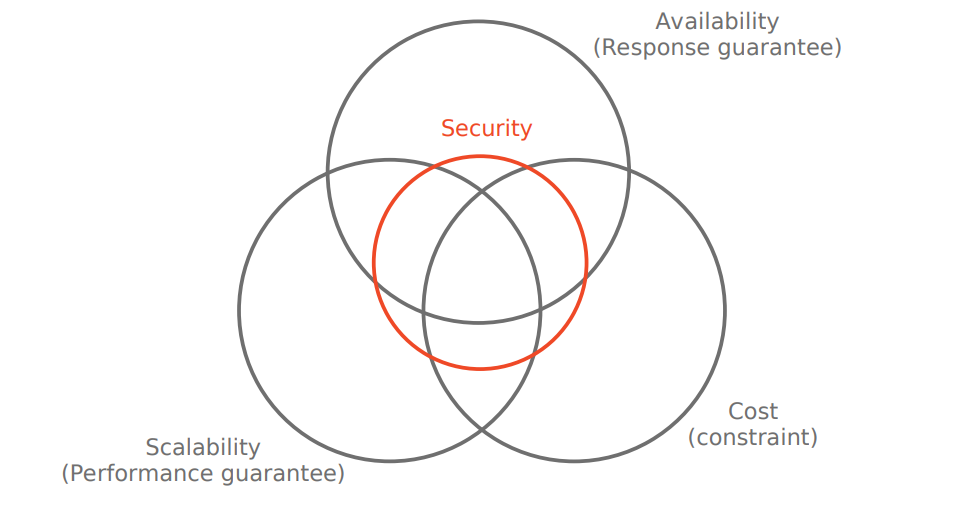
\includegraphics[width=0.8\textwidth]{SAC_01.png}
		\end{figure}
		
		Uno dei problemi principali, che si evolvono con l'evolversi del web e dell'esponenziale crescita dei dati, è la scalabilità.
		Alcune soluzioni applicabili nel passato oggi non lo sono più.\\
		Ad esempio: oggi so come gestire 10 gigabyte di dati, domani saprò gestirne 10 Exabyte?\\
		
		Al giorno d'oggi miliardi di persone hanno più di un dispositivo connesso alla rete, fruendo di milioni di servizi, messi a disposizione da milioni di providers, costruiti su milioni di server, contenenti zettabyte di dati, connessi tramite petabyte di reti.\\
		
		Un altro vincolo importante è la costante attenzione per i reclami dei clienti che possono portare alla perdita di fiducia.
		C'è un cambio di paradigma, se prima il punto di partenza era lo sviluppo di una tecnologia adesso è lo sviluppo di un \textbf{servizio}.
		
		\subsubsection{Definizione di servizi}
		\emph{Definizione}: La capacità di un sistema di fornire in modo \textbf{continuativo} una o più risposte in presenza di specifiche richieste al sistema da parte di un utente.\\
		Un servizio viene detto funzionante fintanto che continua a fornire delle risposte.\\
		
		Un concetto importante introdotto nella definizione è la continuità con cui deve essere erogato il servizio. Possiamo quantificarla in due modi:
		
		\begin{itemize}
		    \item Tramite contratto
		    \begin{itemize}
		        \item SLA: Service Level Agreement in cui ci si accorda sui pagamenti e le penali in caso di mancato adempimento ai requisiti stabiliti
		    \end{itemize}
		    \item Reputazione: La mancata continuità nell'erogazione del servizio porta alla perdita di clienti e di fiducia nei confronti del provider
		\end{itemize}
		Il compito di un ingegnere cloud è quello di implementare un sistema scalabile che garantisca una certa continuità, attraverso i seguenti passi:
		
		\begin{itemize}
		    \item Design
		    \item Build
		    \item Test
		    \item Document
		    \item Monitor
		    \item Fix/Update
		\end{itemize}
		
		Per quanto riguarda invece le linee guida generali a cui attenersi sempre, cosiddette \textit{d'oro}, individuiamo le seguenti:
		\begin{itemize}
		    \item Evitare:
		    \begin{itemize}
		        \item Colli di bottiglia: singoli punti nell'infrastruttura che limitano la capacità totale dell'applicazione
		        \item Single Point of Failure: parte del sistema che, qualora fallisse, influenza tutto l'apparato arrestandolo. Benché non sia facile rimuoverli in certi casi, occorre almeno identificarli.
		        Esempi:
		        \begin{itemize}
		            \item Elettricità e continuità di corrente in un data center.
		        \end{itemize}
		    \end{itemize}
		\end{itemize}
		
		\subsection{Cloud Computing}
		\paragraph{Grid Computing}
		L’architettura \textbf{grid computing} unisce diverse unità geograficamente distanti per determinati intervalli di tempo con uno scopo specifico: i computer comunicano e agiscono come una singola identità di calcolo. Utilizzare un nodo significa quindi accedere alla potenza computazionale di tutta la rete.\\
		
		Il grid computing è una rete che può essere sia omogenea che eterogenea, ovvero formata da nodi con identici o meno. I nodi che compongono l’architettura sono indipendenti: ciascun server o computer mantiene la propria autonomia dalla rete e condivide solo in parte le proprie risorse specifiche. La rete del grid computing è quindi decentralizzata.\\
		
		L'idea principale è quella di un grande supercomputer distribuito in cui molte organizzazioni contribuiscono mettendo a disposizione le proprie risorse. L'unità di lavoro è il \emph{gridlet}.
		
		\paragraph{Globus Toolkit}
		E' un meccanismo per creare sistemi grid, finalizzato al calcolo scientifico e parallelo. Lo scheduling viene eseguito per batch jobs, presentando quindi un'interattività limitata. Assenza di un chiaro modello economico.
		
		\subsection{Gestione delle Risorse}
		E' importante cercare di quantificare l'utilizzo di un server per potere soddisfare il carico richiesto. Quest'ultimo, infatti, può variare sensibilmente nel corso di una giornata e non vogliamo incorrere né in perdite di introiti derivanti dalla \textbf{mancata erogazione del servizio} né nella \textit{sotto-utilizzazione} delle stesse macchine. Un'intuizione vincente fu quella di Bezos che inizio a vendere potenza di calcolo inutilizzata ad altre aziende.\\
		
		Le politiche per gestire la potenza di calcolo in un'azienda sono diverse, si può scegliere di:
		\begin{itemize}
		    \item Soddisfare un workload \textbf{minimo}: riduciamo i costi ma siamo poco appetibili sul mercato
		    \item Soddisfare l'utilizzo \textbf{medio}: non riusciamo a soddisfare il picco della domanda e potrei comunque avere potenza computazione inutilizzata
		    \item Soddisfare il \textbf{picco} della domanda: riesco a guadagnare ottima reputazione tra i clienti, aumentando così gli incassi ma ho molta potenza computazionale inutilizzata
		\end{itemize}
		
		\subsection{Alte performance e realizzabilità}
		Alte performance si possono ottenere solo:
		\begin{itemize}
		    \item Evitando \textbf{overload} e \textbf{bottlenecks}
		    \item Fornendo \textbf{tempi di risposta} accettabili
		\end{itemize}
		Contariamente a quanto si può pensare sulla base delle regole auree dette prima, evitare SPoF (Single Points of Failure) non garantisce alte performance ma realizzabilità.\\
		
		L'obiettivo consiste nel fornire un determinato throughput (rateo di risposte) e un determinato tempo di risposta. I due obiettivi possono essere legati, dove la richiesta di uno prevede la necessità dell'altro.\\
		Osservando una catena di servizi ci basta capire quale unità di elaborazione ha il troughput minore rispetto agli altri per capire quale sarà il collo di bottiglia nella nostra rete.
		
		\begin{figure}[ht]
		\centering
		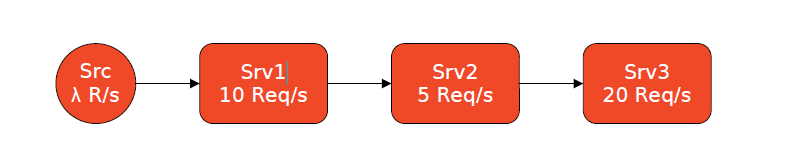
\includegraphics[width=0.8\textwidth]{SAC_02.png}
		\end{figure}
		
		Per ottenere un sistema efficiente che non generi colli di bottiglia bisogna fare in modo che tutti i servizi abbiano lo stesso \textit{data rate}. Un'opzione è quella di replicare i servizi che abbiano un data rate minore, in modo da allinearli al livello degli altri.
		E' importante considerare che se abbiamo del codice che non può essere ne replicabile ne parallelizzabile, non sarà particolarmente adatto ad una struttura basata sul Cloud, per cui potrebbero facilmente generarsi colli di bottiglia.
		
		\subsection{Legge di Amdahl}
		\begin{figure}[ht]
			\centering
			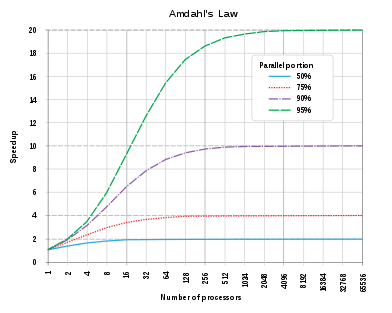
\includegraphics[width=0.5\textwidth]{SAC_03.png}
		\end{figure}
		
		\begin{itemize}
		    \item $Tp$: Tempo richiesto per la parte di elaborazione \emph{parallela}
		    \item $Ts$: Tempo richiesto per la parte di elaborazione \emph{sequenziale}
		    \item $p=\frac{Tp}{Ts+Tp}$: quanto incide la parte parallela sulla computazione totale
		    \item $Tn=Ts+\frac{Tp}{n}$
		    \item $n$: Numero di processori
		\end{itemize}
		\[S=\frac{Ts+Tp}{Ts+\frac{Tp}{n}}\]
		Per n \textrightarrow $\infty$ : \[S=\frac{S}{1-p}\]
		
		
		Il miglioramento delle prestazioni di un sistema che si può ottenere parallelizzando una certa parte del sistema è limitato dalla frazione di tempo in cui tale parte è effettivamente utilizzata
		
		\subsection{Paradigmi del Cloud Computing}
		
		\begin{figure}[ht]
		\centering
		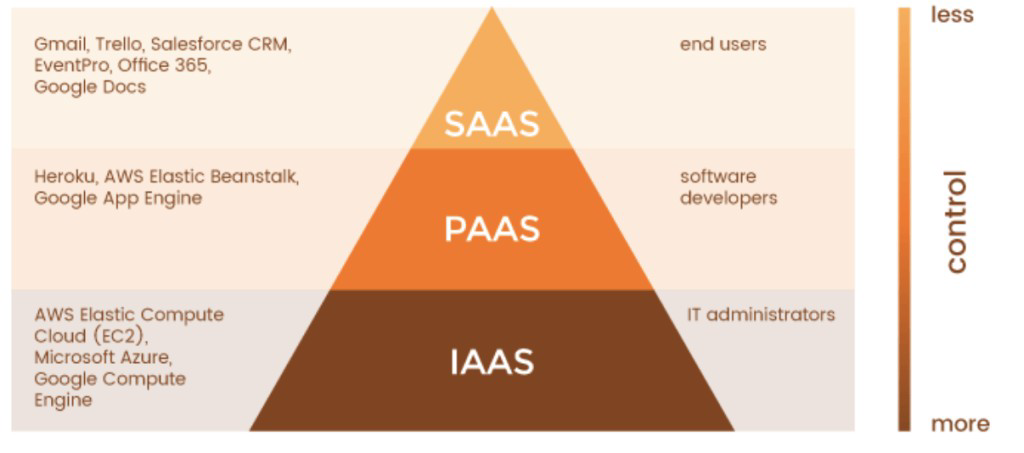
\includegraphics[width=0.5\textwidth]{SAC_04.png}
		\end{figure}
		
		Le principali caratteristiche del cloud computing sono:
		\begin{itemize}
		    \item Service: ogni elemento viene visto e implementato come un servizio. 
		    \item Deployment: in base alle caratteristiche dell'infrastruttura e della proprietà.
		\end{itemize}
		
		\subsubsection{Paradigma Service}
		
		\begin{figure}[ht]
			\begin{minipage}{0.45\textwidth}
			\centering
			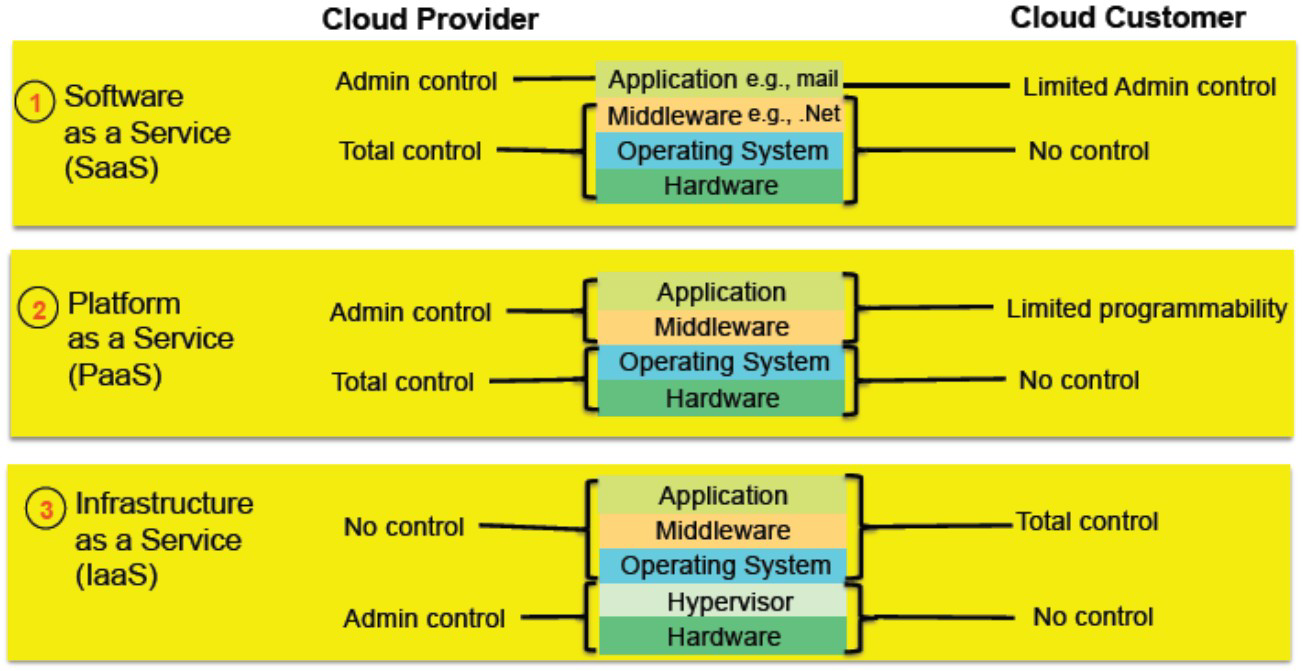
\includegraphics[width=0.8\textwidth]{SAC_05.png}
			\end{minipage}
			\begin{minipage}{0.45\textwidth}
				\centering
				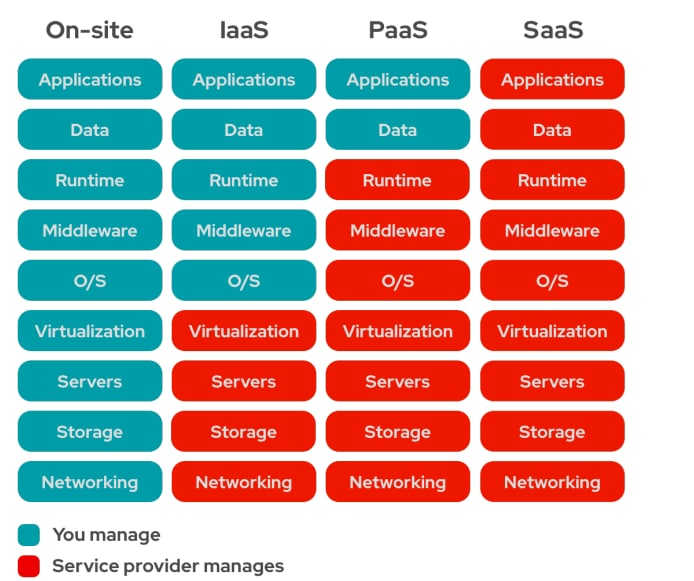
\includegraphics[width=0.8\textwidth]{SAC_A2_service_paradigm.jpg}
			\end{minipage}
		\end{figure}
		
		In base al paradigma scelto sono disponibili differenti livelli di controllo:
		\begin{itemize}
		    \item Software: è la forma più completa di servizi di cloud computing, che fornisce un'intera applicazione gestita dal provider, tramite un browser web.
		    Gli aggiornamenti del software, le correzioni dei bug e la manutenzione generale del software sono gestiti dal provider e l'utente si connette all'applicazione tramite una dashboard o un'API. Non è necessaria l'installazione del software sui singoli computer e l'accesso di gruppo al programma è più fluido e affidabile.
		    \item Platform: Il provider ospita l'hardware e il software sulla propria infrastruttura e fornisce questa piattaforma all'utente come soluzione integrata, stack di soluzioni o servizio attraverso una connessione Internet. All'ambiente per costruire e distribuire ci pensa il provider.
		    \item Infrastructure: Si tratta di un servizio pay-as-you-go in cui una terza parte fornisce all'utente servizi di infrastruttura, come lo storage e la virtualizzazione, in base alle sue esigenze, tramite un cloud, attraverso Internet.
		    L'utente è responsabile del sistema operativo e di tutti i dati, le applicazioni, il middleware e i runtime, mentre il provider gli fornisce l'accesso e la gestione della rete, dei server, della virtualizzazione e dello storage di cui ha bisogno. 
		\end{itemize}
		
		
		Al giorno d'oggi la differenza tra Software e Platform è sfumata, basti pensare a quanti software forniti come servizi cloud possono essere altamente personalizzati come SAP, Salesforce e Shopify. Il confine è labile anche nell'altra direzione in cui molte piattaforme possono diventare quasi delle infrastrutture.
		
		\newpage
		\subsubsection{Paradigma del deployment}
		
		\begin{figure}[ht]
		    \centering
		    \begin{minipage}{0.45\textwidth}
		        \centering
		        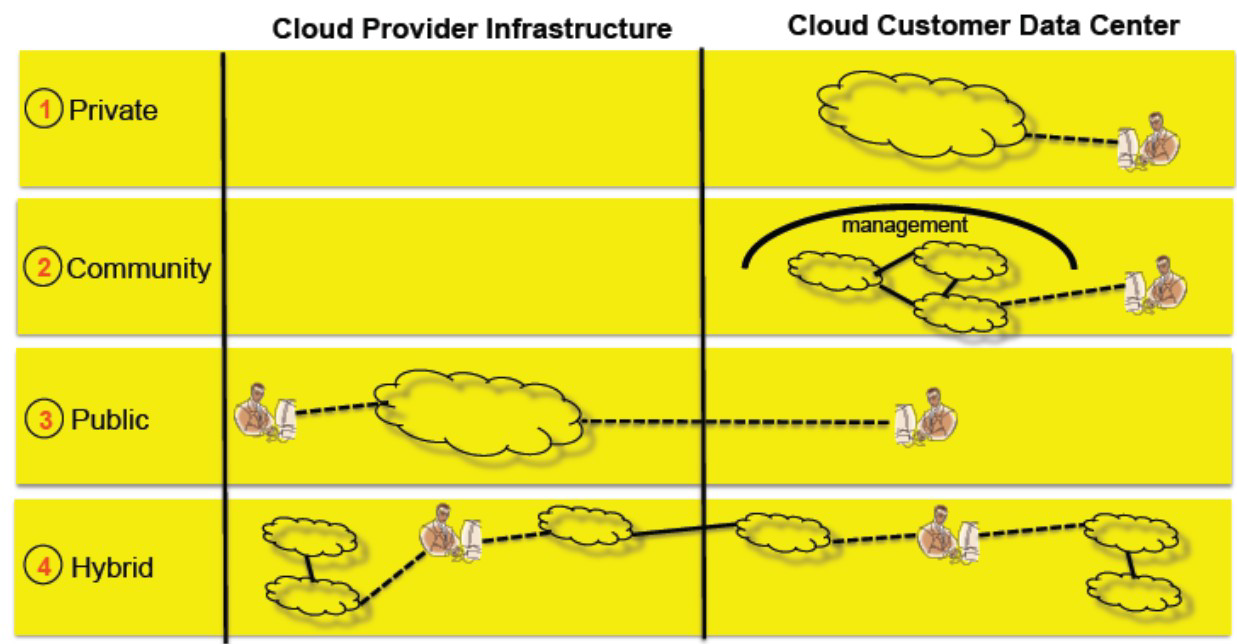
\includegraphics[width=0.9\textwidth]{SAC_06.png} % first figure itself
		    \end{minipage}\hfill
		    \begin{minipage}{0.45\textwidth}
		        \centering
		        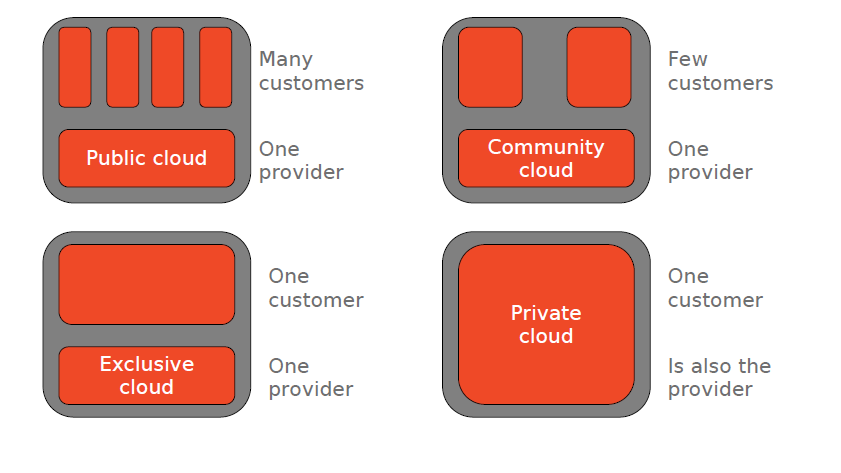
\includegraphics[width=0.9\textwidth]{SAC_07.png} % second figure itself
		    \end{minipage}
		\end{figure}
		
		\begin{itemize}
		    \item Public Cloud: Un cloud pubblico offre i suoi servizi a qualunque utente. Questa struttura deve affrontare il problema della eterogeneità degli utenti, che possono avere bisogni diversi.
		    \item Community Cloud: Gli utenti sono tra di loro più simili. In questo contesto il tipo di servizio è cucito su un determinato tipo di utenza. Da un punto di vista strutturale il cloud può essere ospitato sia dal provider che affidarsi ad un terzo (pubblica amministrazione, assistenza sanitaria)
		    \item Private Cloud: In questo caso tutto il lavoro svolto dal cloud sarà solo ed esclusivamente legato all'azienda/entità.
		    Può essere gestito sia dall'azienda che da terzi
		    \item Hybrid: Mix tra le tipologie precedenti. Ad esempio possono essere più cloud (privati) federati tra di loro che devono svolgere compiti simili, o cloud privati che si appoggiano a cloud pubblici per gestire determinati compiti che possono generare dei picchi di richieste normalmente insoddisfabili. (Amazon).
		\end{itemize}
		
		\subsubsection{Strutture del cloud}
		\paragraph{Vertical Silos}
		\begin{wrapfigure}{r}{0.4\textwidth}
			\centering
			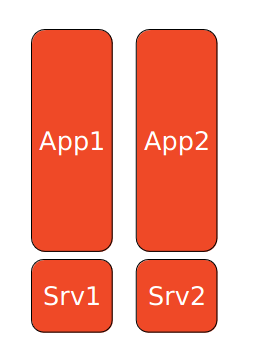
\includegraphics[width=0.6\linewidth]{SAC_A2_verticalsilos}
			\label{fig:saca2verticalsilos}
		\end{wrapfigure}
		
		Tipico approccio di deployment di un'applicazione, non è proprio una struttura cloud, ma è stata la prima implementazione simile.
		Architettura one-to-one, dove ad ogni server corrisponde un'applicazione.\\
		Si può cercare di consolidare i vari server in un singolo e creare della macchine virtuali su cui far girare le applicazioni, tuttavia i server rimangono spesso sotto utilizzati.
		
		\subsubsection{Visione del cloud}
		Il consumatore dal suo punto di vista vede:
		\begin{itemize}
		    \item Un set isolato di risorse
		    \item Elastico e scalabile
		    \item Sicuro
		    \item Affidabile
		    \item Con costi abbordabili: pay-per-use
		\end{itemize}
		
		\emph{Definizione}: Il cloud computing è un modello per l'accesso immediato a un set di risorse di computing condivise e configurabili (rete, server, storage, applicazioni e servizi) che possono essere rapidamente forniti e impiegati con il minimo costo di gestione e l'interazione del servizio provider. 
		
		\subsection{Caratteristiche del Cloud}
		Per capire il passaggio a infrastrutture Cloud nell'utilizzo odierno dell'informatica è importante capire quali sono le motivazioni di ciò e i requisiti che il Cloud ha soddisfatto.
		
		\subsubsection{Requisiti}
		E' assolutamente necessario che il software implementato funzioni bene indipendentemente dal \textbf{numero di utenti} che lo stanno utilizzando, garantendo prestazioni, affidabilità e robustezza. 
		Per soddisfare questi requisiti si può ricorrere ad una maggiore potenza di calcolo o alla diminuzione dei costi di trasmissione, ma queste sono vecchie soluzioni. Le nuove soluzioni hanno l'obiettivo comune di doversi adattare rapidamente ai cambiamenti e al bisogno di \textbf{elasticità}, in quanto l'utilizzo di un sistema cloud può essere molto variabile.
		L'elasticità consiste nel sapere trovare un \textbf{equilibrio} tra i costi di infrastruttura e i tempi di esecuzione.
		
		\subsubsection{Software Cloud}
		Per ottenere tale elasticità è opportuno evitare errori come colli di bottiglia, SPOF e comportamenti sincroni. 
		E' sempre bene usare pratiche di replicazione e orchestrazione autonoma.
		A livello di programmazione non è possibile applicare concetti classici come appunto quello della sincronizzazione.
		Per esempio i dati stessi non posso godere di una \textbf{consistenza} totale, avendo quindi in ogni punto del software dati aggiornati e pronti all'elaborazione.
		Lo stesso discorso vale per la comunicazione che non può essere totalizzante e asincrona in ogni momento. 
		Ecco perché per il cloud è opportuno adottare diversi paradigmi a livello software:
		
		\begin{itemize}
		    \item Parallelismo su larga scala.
		    \item Dati:
		    \begin{itemize}
		        \item Lazy consistency: I dati non vengono aggiornati sempre immediatamente.
		        \item Distribuzione locale o geografica.
		        \item Caching
		    \end{itemize}
		    \item Comunicazione:
		    \begin{itemize}
		        \item Asincrona
		        \item IPC (Inter Process Comunication) limitate.
		    \end{itemize}
		\end{itemize}
		
		Vi sono varie funzioni logiche da implementare all'interno del cloud:
		\begin{itemize}
		    \item Database (Model).
		    \item Presentazione (View).
		    \item Aziendale (Controller)
		\end{itemize}
		La replicazione può avvenire sia in modo verticale che orizzontale, ma anche in maniera ibrida. 
		
		\subsection{Architetture}
		Per quanto riguarda invece l'architettura di un servizio gli approcci possibili sono i seguenti:
		\begin{itemize}
		    \item Monolitico: Un singolo software, difficile da replicare e mantenere, quindi costoso. 
		    \item SOA: Service Oriented Architecture. Architettura basata su protocolli SOA e su XML
		    \item Microservizi: Consiste nel suddividere l'architettura in tanti piccoli servizi facili da replicare e impiegare ma sopratutto da implementare
		    \item Serverless: Architettura senza server, una sorta di microservizi 2.0
		\end{itemize}
		
		\begin{figure}[ht]
		\centering
		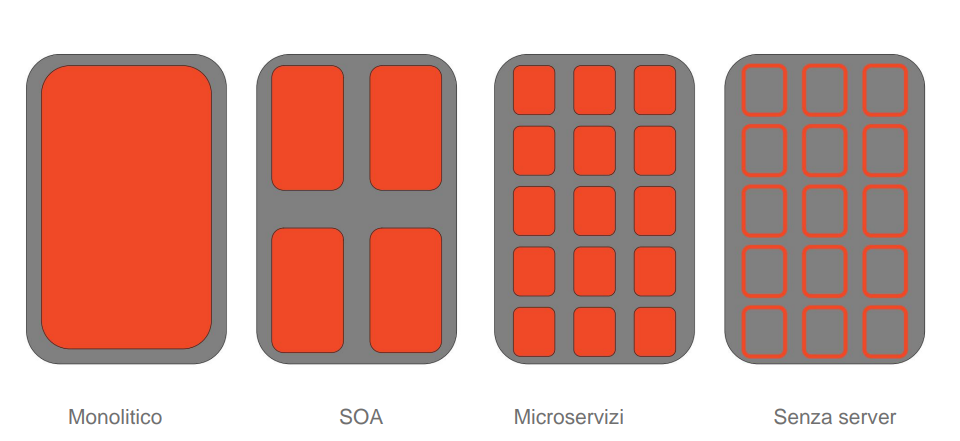
\includegraphics[width=0.8\textwidth]{SAC_A2_architecture_server.png}
		\end{figure}
		Le architetture ibride prevalgono nella maggior parte delle aziende per la difficoltà di queste a convertirsi ai nuovi paradigmi.
		
		\subsubsection{Modelli pre-SOA}
		
		Prima dell'avvento della Service Oriented Architecture le possibilità erano:
		\begin{itemize}
		    \item RPC: Chiamata di procedura remota. Consiste nella creazione di codice per astrarre un'invocazione remota, nascondendo gli aspetti dell'interazione remota. Viene usato il linguaggio IDL
		    \item RPC orientato agli oggetti.
		    \item Middleware orientato ai messaggi: Approccio client-server con messaggi sincroni o asincroni con code di messaggi. Tipici di applicazioni \textit{fire-and-forget} come le notifiche.
		\end{itemize}
		
		Dal punto di vista semantico, una chiamata di funzione locale e la RPC sono la stessa cosa poiché grazie al codice \emph{stub} la complessità è nascosta.
		
		\begin{figure}[ht]
			\centering
			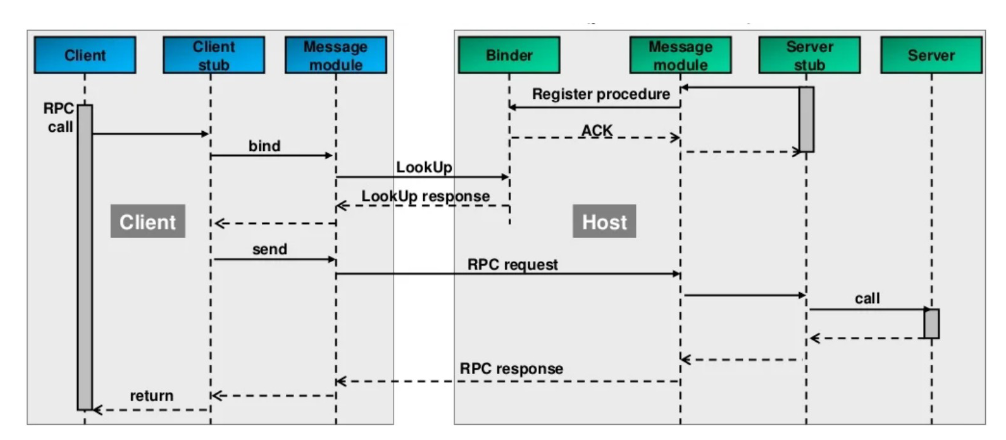
\includegraphics[width=0.8\linewidth]{SAC_A3_rpc}

			\label{fig:saca3rpc}
		\end{figure}

		Il codice \emph{stub} è una porzione di codice che simula il comportamento di un altro software:
		\begin{itemize}
		\tightlist
			\item Il client chiama lo \textbf{s}tub del client. La chiamata è una chiamata di procedura locale, con i parametri inseriti nello stack nel modo normale.
			\item Lo stub del client impacchetta i parametri in un messaggio ed effettua una chiamata di sistema per inviare il messaggio. L'impacchettamento dei parametri è chiamato \textbf{marshalling}.
			\item Il sistema operativo locale del client invia il messaggio dalla macchina client alla macchina server.
			\item Il sistema operativo locale della macchina server passa i pacchetti in arrivo allo stub del server.
			\item Lo stub del server scompatta i parametri dal messaggio. Lo scompattamento dei parametri è chiamato unmarshalling.
			\item Infine, lo stub del server chiama la procedura del server. La risposta ripercorre gli stessi passi in senso inverso.
		\end{itemize}
		
		\paragraph{OO-RPC}
		E' possibile anche ricreare il concetto di RPC nella programmazione orientata agli oggetti, come per esempio in JAVA dove viene definita un'interfaccia che definisce i metodi che vogliamo esporre. La classe che implementa l'interfaccia è l'analogo dell'IDL. 
		
		\subsubsection{Modelli SOA}
		Architettura orientata ai servizi con approccio rivolto al business, è basata su componenti software creati con l'obiettivo di evitare software monolitici e nascondere l'architettura centrale sottostante. 
		In questo modo servizi della stessa azienda possono essere riutilizzati o integrati con altri di altre aziende.
		Si possono avere così tre scenari:
		\begin{itemize}
		    \item SOA intra-aziendali.
		    \item SOA inter-aziendali con rapporti B2B. Un esempio è EXPEDIA che cerca e confronta varie offerte di altre aziende (compagnie aeree).
		    \item SOA inter-aziendali con servizi offerti liberamente.
		\end{itemize}
		Gli elementi che caratterizzano i SOA sono:
		\begin{itemize}
		    \item Servizio: fatto da moduli, deve avere una descrizione e un interfaccia di accesso.
		    \item Tecnologie abilitanti.
		    \item Governance e politiche SOA.
		    \item Metriche SOA.
		    \item Modello organizzativo e comportamentale.
		\end{itemize}
		
		\subsubsection{Service Oriented Architecture Protocol}
		Nasce nell'ambito dei servizi web come tecnologia per la messaggistica di base.\\
		Un servizio Web è un sistema software identificato da un URI, le cui interfacce e collegamenti pubblici sono definiti e descritti utilizzando XML. La sua definizione può essere vista da altri sistemi software.
		Questi sistemi possono quindi interagire con il servizio Web nel modo stabilito dalla sua definizione, utilizzando messaggi basati su XML trasmessi dai protocolli Internet.
		Il protocollo SOAP è basato sui protocolli HTTP o HTTPS e i dati sono scritti attraverso il linguaggio XML.
		
		\begin{figure}[ht]
		    \centering
		    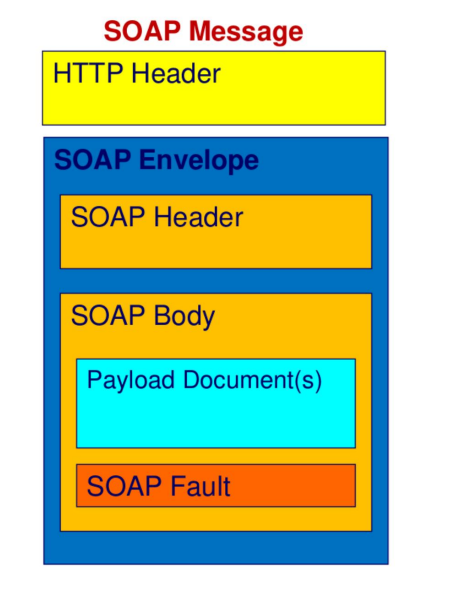
\includegraphics[width=0.5\linewidth]{SAC_A2_soapMessage.png}
		    \caption{Soap è incapsulato in HTTP e definisce una struttura per le risposte HTTP in XML}
		\end{figure}
		
		Tuttavia SOAP presenta dei limiti: la lentezza di XML rappresenta la sua debolezza maggiore. Un approccio migliore è utilizzare JSON che è particolarmente adatto alle architetture REST.
		
		\subsubsection{Enterprise Service Bus}
		L'architettura SOA prevede che i componenti delle applicazioni possano essere lanciati su diverse macchine e debbano essere tutti capaci di comunicare fra loro. Tuttavia all'aumentare del numero di applicazioni, la struttura diventa difficile da mantenere.
		\newline
		L'uso di un middleware \textit{a mo} di BUS condiviso per la connessione tra i componenti permette di interconnettere i vari servizi. Questo componente si chiama ESB (Enterprise Service Bus) e ha le seguenti funzioni
		\begin{itemize}
		    \item Instrada i messaggi verso la destinazione.
		    \item Gestisce differenti modelli di comunicazioni (code asincrone, messaggi in base agli eventi, servizi vari).
		    \item Servizi di intermediazione (broker).
		    \item Connettore e ponte per diversi protocolli.
		    \item Supporta la policy e la qualità del servizio (QoS).
		    \item Monitor, Logging, Sicurezza.
		\end{itemize}
		
		\subsubsection{Microservizi}
		L'architettura a microservizi cerca di mappare l'applicazione in vari elementi molto piccoli, quasi atomici.
		Ogni microservizio ha un suo processo, un suo stack tecnologico diverso (diverso linguaggio di programmazione). All'interno dell'applicazione deve quindi essere implementato un sistema di comunicazione tra i vari servizi.
		
		\paragraph{SOA vs Microservizi}
		Entrambe le strutture supportano complesse applicazioni modellate in maniera più piccola e più maneggevole con parti indipendenti. Alcuni libri considerano i due approcci identici.
		I microservizi comunicano molto bene attraverso le API e non richiedono un ESB. Ognuno può essere aggiornato e spento singolarmente (se non usato al momento).
		La separazione logica tra i microservizi permette la loro esecuzione all'interno di containers.
		\newline \newline
		Benefici
		\begin{itemize}
		    \item Migliore testing: I servizi sono piccoli e facili da testare
		    \item Deployment: Possono essere caricati indipendentemente
		    \item Organizzazione: Rende più facile l'organizzazione del lavoro tra team e ogni team può organizzare e gestire il proprio microservizio. 
		\end{itemize}
		Difetti
		\begin{itemize}
		    \item Non tutte le applicazioni sono orientate a microservizi.
		    \item Non è così diffuso in scenari tradizionali.
		    \item Un'applicazione deve implementare la comunicazione tra servizi.
		    \item Overhead: se non implementati a dovere si rischia di mandare in crash il sistema.
		\end{itemize}
		
		\subsection{Architettura REST}
		\subsubsection{Applicazioni Cloud}
		Ricordiamo che le applicazioni cloud hanno i seguenti requisiti:
		\begin{itemize}
		    \item Resilienza
		    \item Resistenti a failures
		    \item Elastici in modo da scalare da pochi server a decine di migliaia.
		    \item L'architettura deve avere dei servizi \textit{loosely-coupled} e stateless
		\end{itemize}
		
		\subsubsection{REST}
		REpresentation State Transfer, fornisce all'applicazione un architettura senza stati, utilizzando tutti i \textbf{verbi} del protocollo HTTP.
		Il concetto chiave è quello di incapsulare una risorsa all'interno di un'entità (URI). Le risorse forniscono dati attraverso una rappresentazione (come ad esempio una struttura JSON). Le azioni sulle varie entità sono mappate su messaggi (cioè i vari metodi del protocollo HTTP). Non necessita di molteplici servizi ausiliari per il funzionamento.
		
		\begin{figure}[ht]
		\centering
		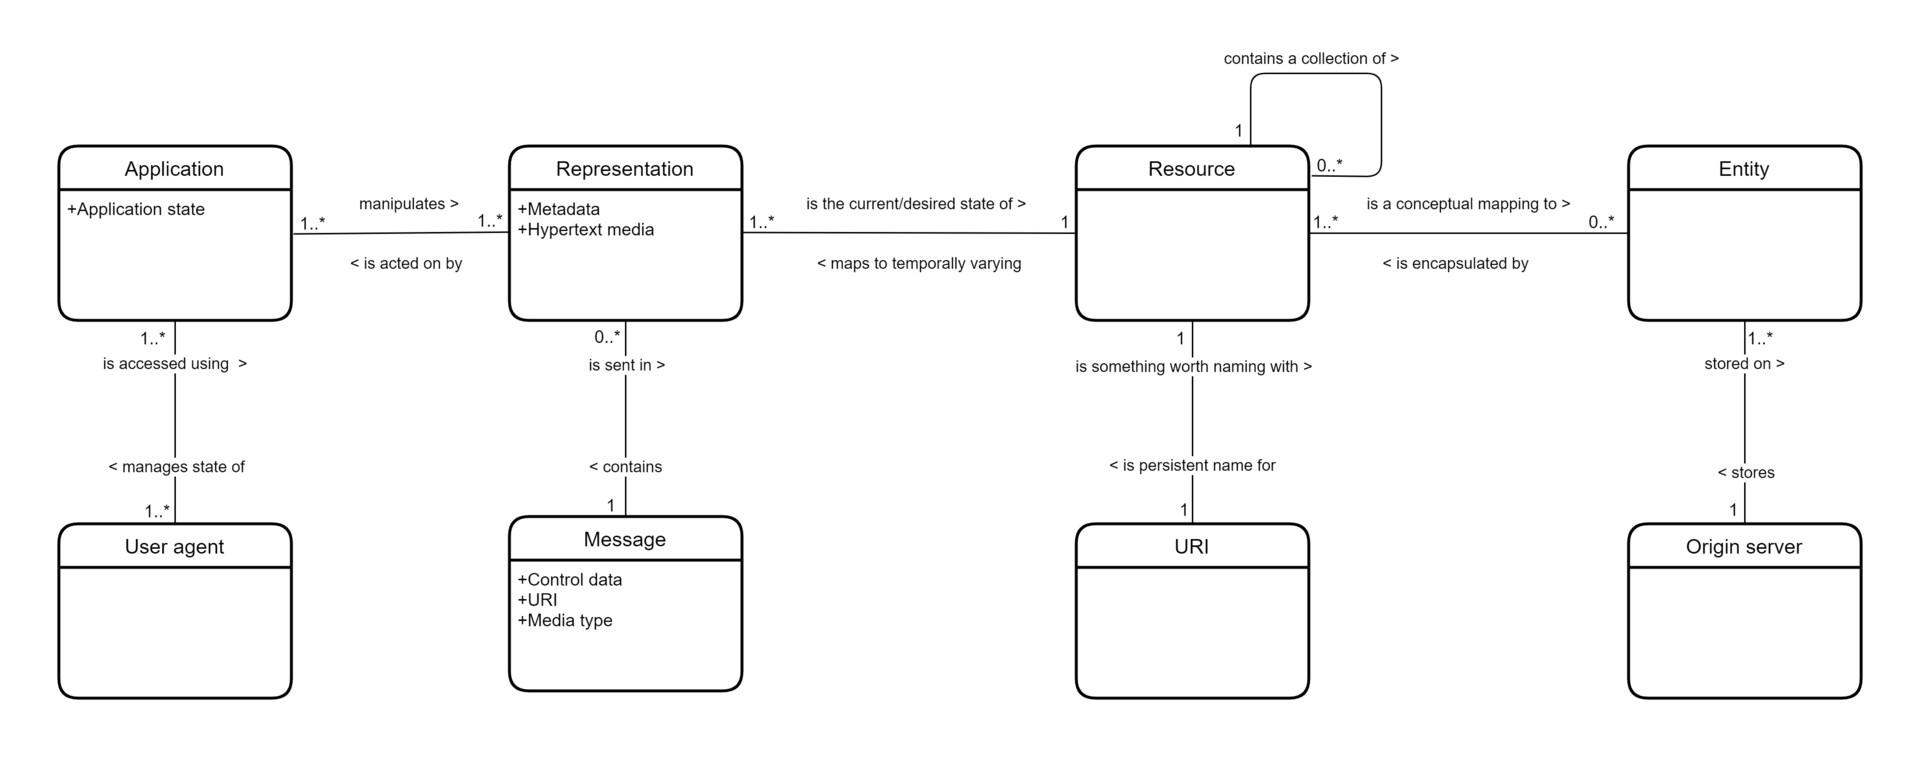
\includegraphics[width=0.9\textwidth]{SAC_08.png}
		\end{figure}

		I client e i server sono molto leggeri dato che le risorse, identificate da URI, incapsulano delle entità e per invocarle non c'è bisogno di una SOAP. In questo caso il contenuto delle risorse viene visualizzato con una struttura chiave valore, stile JSON.
		Vincoli
		
		\begin{itemize}
		    \item Modello client server.
		    \item Operazione stateless.
		    \item I risultati possono essere salvati in cache.
		    \item Struttura a strati. 
		    \item Un servizio REST può interfacciarsi con altri servizi. 
		    \item Interfaccia uniforme: L'uso di URI ( Uniform Resource Identifier ), fornisce una rappresentazione delle azioni e dei messaggi autodescrittiva. 
		\end{itemize}
		
		Benché non ci siano espliciti limiti nella configurazione dei messaggi, Le azioni tipiche seguono il paradigma CRUD:
		\begin{itemize}
		    \item CRUD paradigm: 
		    \begin{itemize}
		        \item Create.
		        \item Retrieve (Read).
		        \item Update.
		        \item Delete.
		    \end{itemize}
		\end{itemize}
		
		Le risorse sono accessibile attraverso URL usando i seguenti metodi HTTP:
		\begin{itemize}
		    \item GET: Richiede la risorsa
		    \item POST: Crea un risorsa
		    \item PUT: Modifica la risorsa
		    \item DELETE.
		    \item HEAD: Controlla se una risorsa esiste o è cambiata
		    \item OPTIONS: Quali sono i metodi supportati per una risorsa. 
		\end{itemize}
		
		Ecco i vari codici di risposta delle chiamate REST:
		\begin{figure}[ht]
		\centering
		    \begin{minipage}{0.5\textwidth}
		        \centering
		        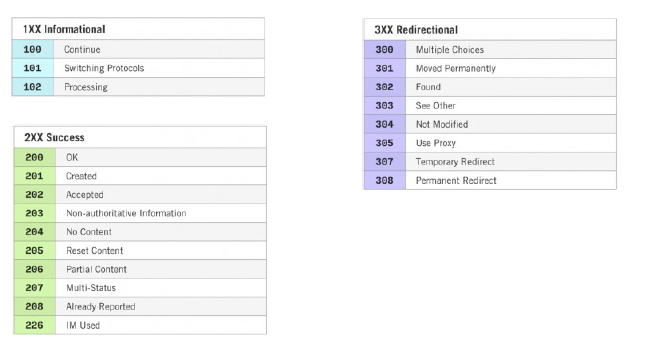
\includegraphics[width=0.9\textwidth]{SAC_09.png} % first figure itself
		        \caption{Information - Succcess - Redirectional}
		    \end{minipage}\hfill
		    \begin{minipage}{0.5\textwidth}
		        \centering
		        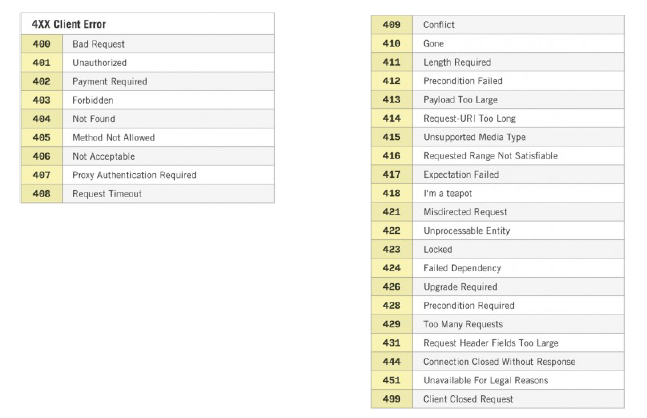
\includegraphics[width=0.9\textwidth]{SAC_10.png} % second figure itself
		        \caption{Client Error}
		    \end{minipage}
		\end{figure}
		
		\begin{figure}[ht]
		    \centering
		    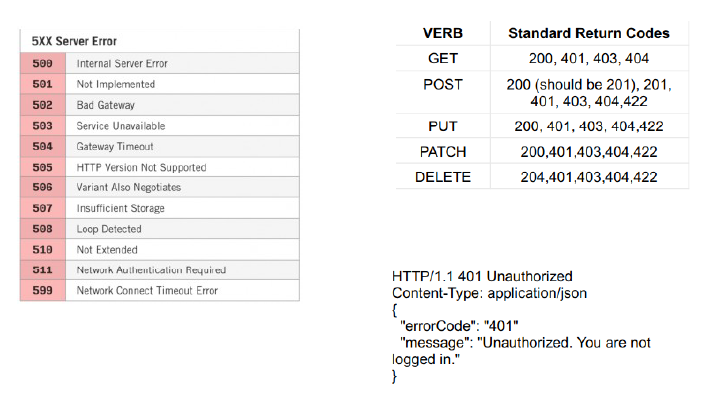
\includegraphics[width=0.9\textwidth]{SAC_11.png}
		\end{figure}
		
		\newpage
		Una richiesta HTTP può essere \textit{cached} in modo da non dover nuovamente essere richiesta al server. E', inoltre, possibile definire un TTL, \textit{time to live}, per stabilire il tempo massimo di esistenza all'interno della cache.\\
		Un \textit{Etag} mantiene i metadati sulla risorsa e sull'ultima modifica ad essa fatta tramite un MD5 digest della rappresentazione della risorsa, tramite cui viene verificato se la risorsa cached è aggiornata o meno.

		\subsubsection{RESTful API}
		Rappresenta lo standard \textit{de facto} per la costruzione di sistemi distribuiti.\\
		I servizi REST non hanno supporto diretto per generare un client da un IDL (termine generico per indicare un linguaggio che consente a un programma di comunicare con un altro scritto in una lingua sconosciuta) mentre i sistemi SOAP possono generare codice STUBS da WSDL (Web Service Description Language), un linguaggio formale in formato XML utilizzato per la creazione di "documenti" per la descrizione di servizi web.\\
		
		Occorre quindi un description language, cioè una specifica implementazione per IDL machine-readable usata per descrivere, produrre e visualizzare RESTful web services. Un esempio è OpenAPI.\\
		
		Un concetto fondamentale delle chiamate REST è il controllo dei media, ovvero del tipo di contenuto disponibile che il client può chiedere e che il server può fornire. 
		L'idea di base è che una rappresentazione di un oggetto dovrebbe dire al cliente cosa può fare con l'oggetto o le azioni correlate che potrebbe intraprendere.
		Tali descrizioni sono chiamate "\textbf{controlli ipermediali}". Il paradigma Hypermedia as the Engine of Application State prevede che l'utente non abbia conoscenza a priori di come interagire con un applicazione e abbia solo una conoscenza generica degli hypermedia.\\
		
		Le public REST APIs devono essere:
		\begin{itemize}
		    \item Semplici e stateless: Non essere legate a processi come i servizi Web.
		    \item Bullet proof: Devono contemplare una gestione degli errori/controllo degli input
		    \item Progettate dall'esterno verso l'interno in modo che i lenti cambiamenti interni non vengano avvertiti dall'esterno
		    \item Auto descrittive: Devono usare documentazione standard per web API (esempio Swagger)
		    \item Riutilizzabili: Devono essere configurabili non codificate
		\end{itemize}
		
		\subsection{Architetture guidate agli eventi (EDA)}
		Alternativa all'architettura REST, si basa sul concetto di evento che guida le interazioni o i risultati. Questo evento può assumere una varietà di forme e la natura di come questi eventi vengono comunicati all'utente finale è spesso l'elemento più significativo che definisce l'implementazione dell'EDA. Sono delle architetture flessibili e reattive che riescono ad adattarsi ai cambiamenti in \textbf{tempo reale}.\\
		
		Gli elementi che generano notifiche non devono necessariamente conoscere i componenti software del ricevente. Il tempo di risposta non è deterministico proprio per la natura di questa architettura.\\
		
		Le notifiche di eventi annunciano una modifica nello stato del sistema, possono essere innescate da:
		\begin{itemize}
		    \item Fonti esterne: Input utente, condizioni ambientali.
		    \item Notifiche interne: Invio di dati per la pipeline workchain etc.
		\end{itemize}
		Un classico esempio applicativo di questa architettura è il sistema Pub/Sub, ma anche:
		\begin{itemize}
		    \item AMQP: Advanced Message Queuing Protocol
		    \item MQTT: Message Queue Telemetry Transport
		    L'architettura prevede, ad esempio, un sensore che rilevando dei dati inerenti a qualche monitoraggio comunica ad un intermediario, il broker, responsabile dell'inoltro dei messaggi ai client destinatari. I messaggi scambiati hanno una struttura chiave-valore.
		    \item Apache Kafka: Si passa dalle entità contenute nei database ad una sequenza di eventi non ordinate descritta nei logs.
		    Gli eventi, infatti, sono molto più adatti a scalare delle entità. Ogni log è associato ad un topic e può essere replicato o partizionato, suddividendolo in sub-log.
		    Kafka è focalizzato sulla scalabilità e la tolleranza a \textit{failure}. Tolleranza che però viene pagata in termine di costi, data la sua replicazione.
		\end{itemize}
		
		\subsubsection{EDA Scalability}
		I punti chiave per la scalabilità delle architettura ad eventi sono la possibilità di inviare messaggi in modo \textbf{asincrono} tra le \textit{loosely couples} che si creano (publisher-subscriber) e la \textbf{consistenza debole}, dove i dati vengono aggiornati non in maniera istantanea ma solo in determinati momenti.
		\begin{itemize}
		    \item Comunicazioni asincrone: Le code vengono utilizzate come dei buffer. I consumatori processano gli eventi come meglio possono e se una applicazione dovesse saturare per il carico eccessivo, rallenterà un po' ma non andrà mai in down.
		    \item Accoppiamento libero: A causa della struttura Pub/Sub, i publisher non sanno nulla riguardo i subscriber che decidono di iscriversi ad un determinato argomento per ricevere le notifiche.
		    \item Eventual Consistency: Utilizza una cache per memorizzare i dati aggiornati, riduce il carico del sistema e mantiene comunque i dati in un buon stato per tutti i nodi dell'architettura. 
		    Il livello di consistenza che si vuole mantenere nel nostro database dipende come sempre dal tipo di applicazione che stiamo creando.
		    Per un social network, un aggiornamento non istantaneo non è un problema, per un sistema di stoccaggio di scorie nucleari forse si. 
		\end{itemize}
		
		L’eventual consistency, se da un lato risulta più debole sia della consistenza del teorema CAP che della consistenza delle transazioni ACID, dall’altro, a regime e con un certo grado di imperfezione, tende a raggiungerle entrambe. Infatti la ricezione dei messaggi dai sistemi cooperanti permette sia di replicare in locale i dati aggiornati di pertinenza dei sistemi remoti, sia di adeguare i dati di pertinenza del sistema locale al fine di soddisfare i vincoli di integrità complessivi del sistema distribuito.
		
		\subsection{Comunicazione e Coordinamento}
		Dopo aver visto varie implementazioni di strutture cloud è importante cercare di capire come poterli gestire e orchestrare.
		\begin{itemize}
		    \item Orchestrazione: Un'autorità \textbf{centralizzata} controlla l'esecuzione dei servizi dei nodi, proprio come un direttore d'orchestra fa con i musicisti.
		    \item Coreografia: Ogni componente conosce il proprio set di azioni prestabilito che deve compiere in relazione agli altri elementi con cui interagisce. Alla base di questo design vi è l'\textbf{Event Stream}, un bus su cui i componenti pubblicano e ricevono gli uni dagli altri. Questo non è un componente fisico vero e proprio come l'ESB.\\
		    L'analogia è con i ballerini in cui ognuno sa cosa fare in base a come si muove il ballerino prima e dopo di lui. Questo modello di coordinamento è implicitamente \textbf{decentralizzato}.
		\end{itemize}
		
		In entrambi i casi i servizi possono essere incapsulati in REST API, cambia solo il modo in cui vengono gestite le richieste.

		\subsubsection{Resilienza}
		La resilienza è un obiettivo fondamentale dei sistemi distribuiti per evitare il verificarsi di problemi come errori a cascata o chiamate remote fallite, bloccate o senza risposta.
		Quando qualcosa va storto bisogna gestire il tutto arrecando meno danno possibile. Quando abbiamo servizi connessi tra di loro, un problema su uno di essi può, infatti, ripercuotersi su tutti gli altri connessi.\\
		
		Per evitare questi errori è importante mantenere i nostri servizi il più possibile stateless in modo tale da non perdere informazioni in caso di interruzione del servizio.
		Se viceversa si ha un servizio con stato, la migrazione è molto più complicata e in quel caso si perdono informazioni. Ad esempio un utente in un e-commerce perderebbe tutti i prodotti inseriti in un carrello.\\
		
		Un'altra caratteristica importante è quella di scrivere delle chiamate REST robuste e capaci di gestire errori e ritardi.\\
		
		\begin{wrapfigure}{r}{0.5\linewidth}
			\centering
			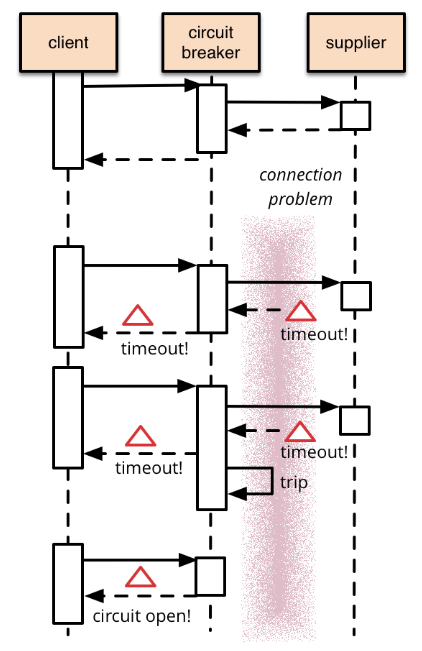
\includegraphics[width=0.4\linewidth]{SAC_A3_breakers}
			\label{fig:saca3breakers}
		\end{wrapfigure}
		\paragraph{Circuit Breakers}
		
		I Circuit Breakers sono un modello di progettazione utilizzato nello sviluppo del software. Vengono utilizzati per rilevare i guasti e prevedono una logica per evitare che questi si ripetano costantemente.\\
		
		Il circuit breaker funge da intermediario per le operazioni che potrebbero fallire. Questo deve monitorare il numero di fallimenti recenti che si sono verificati e utilizzare queste informazioni per decidere se consentire all'operazione di procedere o se restituire immediatamente un'eccezione, marcando il servizio come \textbf{bad}.
		
		\newpage
		\section{Data Management}
		\paragraph{Data Replication}
		
		La scalabilità si può ottenere tramite:
		\begin{itemize}
			\item Scale-Up: Tramite il miglioramento delle risorse hardware del server. Presenta degli ovvi limiti fisici, risolvibili solo tramite lo scale out.
			\item Scale-Out: Lo scaling orizzontale prende l'infrastruttura esistente e la replica per lavorare in parallelo. Questo ha l'effetto di aumentare la capacità dell'infrastruttura in modo approssimativamente lineare. Scalando orizzontalmente si ha una replicazione a livello di storage, per cui bisogna stabilire come quest'ultimo venga aggiornata.
		\end{itemize}
		
		\begin{figure}[ht]
			\centering
			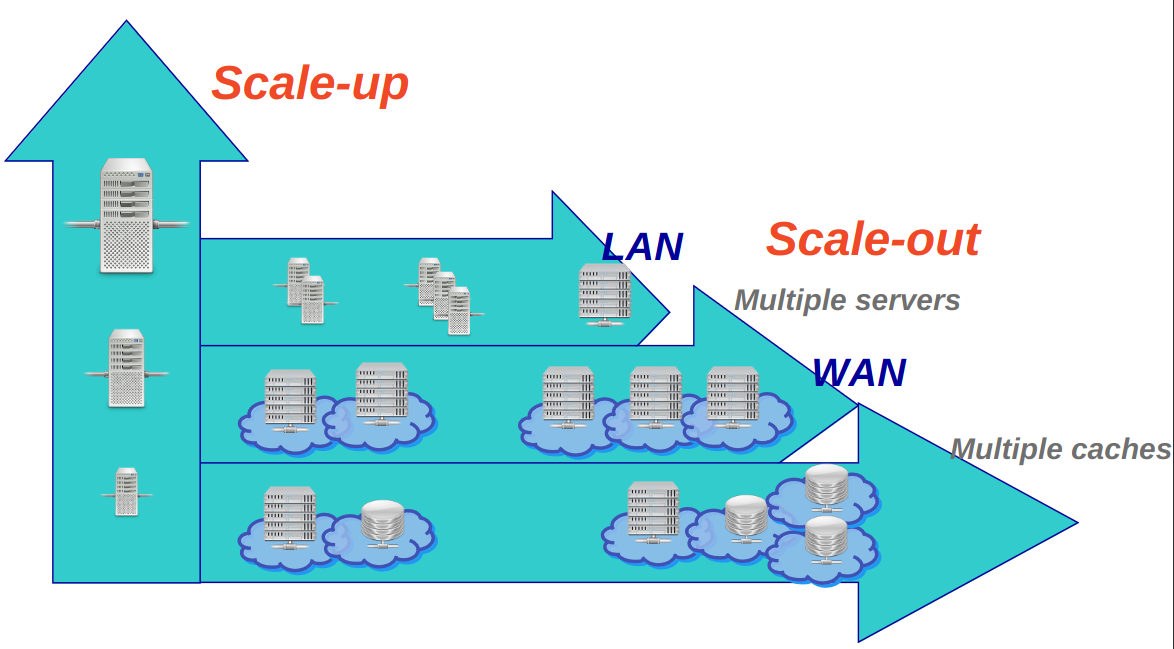
\includegraphics[width=0.65\linewidth]{SAC_A5_scaling}
			\label{fig:saca5scaling}
		\end{figure}
		
		\begin{itemize}
		    \item Replicazione:
		    \begin{itemize}
		        \item Piena: Tutte le risorse vengono replicate.
		        \item Parziale: Soltanto una parte viene replicata.
		    \end{itemize}
		    \item Policy sulla consistency: \begin{itemize}
		        \item Strong: I contenuti sono sempre aggiornati.
		        \item Weak: I contenuti non sono aggiornati immediatamente.
		    \end{itemize}
		\end{itemize}
		
		\subsection{Data Synchronization}
		Se non abbiamo nessuna consistenza si hanno performance migliori, una migliore scalabilità e assenza di overhead dovuto alla sincronizzazione ma ovviamente non è adatto a nessuno scenario in cui vi sia replicazione.
		Se invece abbiamo consistenza forte gli aggiornamenti sono immediati e non c'è rischio di perdere dei dati: è un paradigma adatto a servizi che necessitano di alta disponibilità. Il compromesso che nasce tra i due è la consistenza debole.\\
		
		Possiamo avere due differenti tipi di copie:
		\begin{itemize}
		    \item Primarie: Copie autoritarie.
		    \item Master: Copie in lettura/scrittura.
		\end{itemize}
		Tutte le altre copie che non siano primarie o master sono in sola lettura. Nel caso di consistenza \textbf{forte} tutte le copie sono primarie.
		
		\subsubsection{Concurrency control system}
		\paragraph{One-Copy System} L'idea alla base è che tutte le copie fisiche dei dati si devono comportare come un singolo elemento logico. La sequenza di transazioni distribuite deve essere uguale all'esecuzione serializzata delle stesse sullo stesso elemento logico. Il che significa che quando leggiamo un dato questo deve essere il risultato della scrittura più recente dalla precedente transazione nell'equivalente ordine seriale.\\
		
		Ad esempio, se io prelevo contemporaneamente dallo stesso conto 20 euro in America e 20 euro in Europa e il mio bilancio iniziale era di 50 euro, vorrei che il bilancio finale fosse di 10 euro. Poiché posso ipotizzare che entrambe le filiali abbiano la propria copia del database dei conti correnti, il bilancio potrebbe non essere sempre 10 euro, ma 30 euro.\\		
		
		Il sistema one-copy prevede che le transizioni vengano effettuate sulla stessa copia logica, risolvendo quindi il problema. 
		La coerenza delle copie è garantita da un sistema di controllo che assicura il corretto funzionamento, dopo l'avvenuta sincronizzazione.	
		
		\paragraph{Two-phase commit}
		E' un'altra strategia di sincronizzazione che ha bisogno di un \textbf{coordinatore} che prenda la decisione finale e interagisca con ogni partecipante. Può esserci anche un approccio gerarchico in cui il coordinatore delega i nodi primari di interpellare i nodi finali.
		Si basa su due fasi:
		\begin{itemize}
			\item Preparazione: in cui il coordinatore prepara tutte i partecipanti ad eseguire la transizione e attende che questi rispondano con l'esito dell'operazione.
			\item Scrittura: in cui, sulla base dei voti dei partecipanti, il coordinatore decide se continuare nella transazione o interromperla e avvisa i partecipanti dell'esito della decisione. I partecipanti seguiranno le indicazioni facendo o meno rollback a prima del commit.
		\end{itemize}
		\begin{figure}[ht]
			\centering
			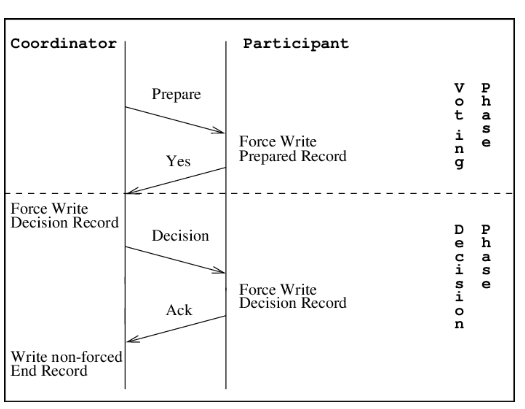
\includegraphics[width=0.5\linewidth]{SAC_A5_twophase}
			\label{fig:saca5twophase}
		\end{figure}
		Creato per la sincronizzazione di database distribuiti, fornisce un forte supporto di coerenza ma è relativamente costoso. Inoltre il rischio di una rollback aumenta il numero di repliche e il numero di messaggi scambiati.
		
		\paragraph{Gossip Protocol}
		Un sistema di replicazione dati basato su scambi di informazioni con i vicini. L'approccio alla consistenza è dato dal fatto che ci sono almeno N repliche di ogni elemento, dove N può essere configurato e $\mathbf{N > 1}$ indica alta disponibilità dell'elemento.\\
		
		Un esempio è Cassandra: quando un nodo riceve una query, identifica tutti i nodi che replicano l'elemento interessato attraverso una DHT (\textbf{Distributed Hash Table}). Invia quindi un aggiornamento della replica ai nodi trovati. In questo caso abbiamo una consistenza \textit{lazy} perché prima o poi la propagazione delle modifiche si estenderà a tutti i nodi.
		
		\paragraph{Primario e secondario}
		In questo sistema il server secondario può rispondere solo nel caso di failure del server primario, garantendo quindi availability. Alternativamente può essere utilizzato per fornire performance aggiuntive. Le operazioni di scritture devono essere inviate al server primario che procederà successivamente a sincronizzare i server secondari, con una periodicità variabile (da pochi minuti a diversi giorni). Tuttavia la copia nel server secondario viene utilizzata solo se la copia primaria non è disponibile.
		
		\subsubsection{Consistenza forte e debole}
		Le coppie di repliche primarie-primarie mantengono una consistenza forte venendo aggiornate immediatamente, mentre una coppia primaria-secondaria ha una consistenza \textbf{debole}.\\
		Nei server secondari si può avere una perenne consistenza debole ma prima o poi i dati convergeranno ad un'unica versione e le copie saranno coerenti. Per fare ciò vi è uno scambio periodico di dati con \textbf{timestamp}, un algoritmo inventato da Lamport per ordinare i messaggi.\\
		
		Vi sono due approcci per regolare la consistenza nel nostro database:
		\begin{itemize}
		    \item BASE
		    \subitem Basic Availability: La replica dei dati riduce il rischio dell'indisponibilità e il partizionamento dei server. Il sistema risulta così sempre consultabile. 
		    \subitem Soft-State: I dati possono essere incoerenti e i servizi devono tenerne conto. 
		    \subitem Eventual Consistency: Prima o poi nel futuro i dati saranno coerenti ma non c'è garanzia di quando questo accada.
		    \item ACID: Atomicity, Consistency, Isolation, Durability. Tipico approccio dei database relazionali.
			\begin{itemize}
				\item I processi devono essere transazionali, totali o nulli.
				\item Dati sempre coerenti dopo una transazione.
				\item Database isolato e indipendente dalle transazioni
				\item Database robusto alla possibilità di perdita di cambiamenti. Ogni volta che si esegue una transazione i cambiamenti vengono salvati prima di essere effettivamente scritti nei registri di log.
			\end{itemize}
		\end{itemize}
		
		\subsection{Replicazione Geografica}
		Risulta impossibile distribuire server primari in ognuno dei 60000 Autonomous Systems e riuscire a gestirne la consistenza. Per questo si utilizzano un numero sempre crescente di server secondari, utili anche al miglioramento delle performance.
		
		\paragraph{Cache}
		Il caching dei dati avviene su più livelli: hardware, OS, software ma anche a livello browser, server e intermediari. L'obiettivo del caching è quello di \textbf{replicare} parte del contenuto originale in posizioni il più possibile vicine all'utilizzatore.
		I principi su cui si basa il caching sono due:
		\begin{itemize}
			\item Località spaziale: se un utente accede a un dato è molto probabile che i futuri accessi siano nelle immediate vicinanze di quello stesso dato.
			\item Località temporale: se un utente accede a un dato è molto probabile che accederà allo stesso dato a breve e non in un futuro remoto
		\end{itemize}
		
		L'efficacia del caching si basa su tre metriche: \textit{cache hit} se trovo il dato in cache, \textit{cache miss} se non lo trovo e \textit{cache hit rate} ovvero il numero di \textit{hit} in un intervallo di tempo rispetto al numero totale di richieste in quello stesso intervallo.\\
		
		Vi sono vari meccanismi di memorizzazione nella cache:
		\begin{itemize}
		    \item Pull: Il contenuto viene fornito dal server primario a quello secondario quando quest'ultimo viene interpellato da un utente, e non ne esiste una copia valida in cache. Principalmente utilizzato da ISP e proxy servers.
		    \item Push: I contenuti che vengono richiesti con maggiore probabilità sono attivamente inviati al server secondario. Utilizzato da reverse proxy, proxy che recupera i contenuti per conto di un client da uno o più server, e Content Delivery Network (CDN).
		\end{itemize}
		
		\subsubsection{Replicazioni dei dati}
		\begin{itemize}
		    \item Server Proxy: Dal punto di vista del proxy server, quando questo riceve una richiesta per una risorsa, questa viene prima ricercata nella propria cache locale e in caso negativo viene richiesta al server e salvata nella cache, prima di essere restituita al browser.\\
		    La validità dei dati all'interno della cache si deduce dal tempo di creazione e dall'ultima modifica:
		    \begin{itemize}
		        \item Volatile: Dato vecchio ma modificato recentemente.
		        \item Static: Dato vecchio e modificato tempo fa.
		    \end{itemize}
		    Se si ha un nuovo dato è difficile da stabilire ma si presuppone sia volatile.\\
		    Il popolamento della cache è guidato dalle richieste del client.\\
		    Il proxy server non è molto utilizzato in quanto non gestisce contenuti generati dinamicamente e inoltre non supporta le connessioni HTTPS \textit{end-to-end}.
		    \item Reverse Proxy: Un server virtuale posto di fronte al Web server in modo che possa immagazzinare risorse recenti generate dinamicamente. Può essere replicato e diffuso geograficamente.
		    \item Terze parti: ISP o CDN.
		\end{itemize}
		
		Sia Forward che	Reverse proxy sono in grado di replicare i contenuti popolari, riducono i costi del server di origine, riducono il RTT per i client.\\
		Solo il Reverse proxy può suddividere il carico intelligentemente tra i server di origine e modificare dinamicamente i contenuti per conto dei server di origine, in quanto più vicino al server primario.\\
		Di contro, il Forward proxy riduce i costi legati all'ISP per il client.\\
		
		Da un punto di vista di business possono esserci vari scenari, il fornitore di contenuti:
		\begin{figure}[ht]
			\centering
			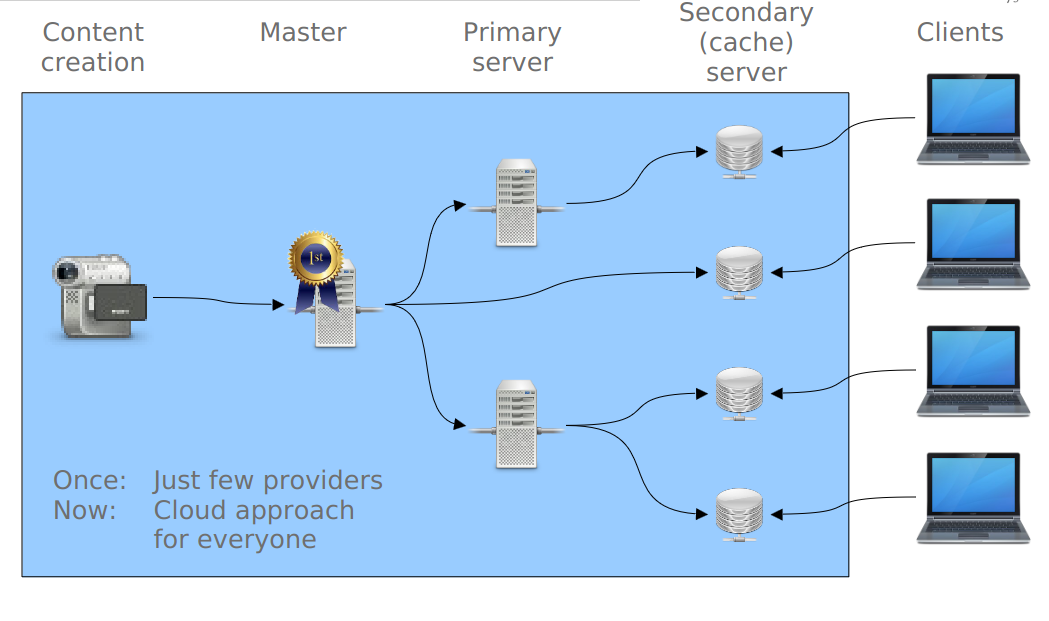
\includegraphics[width=0.7\linewidth]{SAC_A5_contentprovider}
			\label{fig:saca5contentprovider}
		\end{figure}
		
		\begin{itemize}
		    \item Fornisce e gestisce tutto, dalla creazione di contenuti al master, fino a primary e secondary servers.
		    \item Si ferma ai primary servers, delegando i secondary servers.
		    \item Genera contenuti e fornisce il master, delegando il resto a una o più parti
		    \item Genera solo contenuti, delegando tutto a più parti o ad una sola CDN, la quale si occupa dal master fino al secondary.
		\end{itemize}
		
		\subsubsection{Cache WEB}
		Vi possono essere più server proxy che cooperano tra di loro per lo scambio di dati e per aumentare l'hit rate. Se, infatti, un proxy fa hit miss allora può esserci un altro proxy nelle vicinanze che quella risorsa l'ha in cache. Esistono diversi approcci ai proxy server cooperativi:
		\begin{itemize}
		    \item Schema gerarchico: Cooperazione \textbf{verticale}, su più \textbf{livelli}. Dato un miss locale la richiesta viene inoltrata a un nodo nel livello più alto della gerarchia. Ogni livello aumenta però la latenza. Livelli più alti contengono molti più dati per aumentare l'hit rate. Risolve il problema dei \textit{compulsory miss}, cioè quando accediamo ad un dato per la prima volta e quindi questo non è presente in cache
		    \item Schema piatto: Cooperazione \textbf{orizzontale} tra \textbf{pari}. I due approcci tipici sono legati alla rappresentazione dell'informazione:
		    \begin{itemize}
		    	\item Query-based: Quando arriva una richiesta per una risorsa che non ho in cache, la indirizzo ai miei \textbf{vicini}. Il global miss si avrà solo quando tutti i nodi avranno risposto ed ha la stessa velocità del nodo più lento.
		    	\item Informed-based: I vicini si scambiano periodicamente informazioni sui contenuti in cache redigendo un \textbf{indice della cache}. Quest'ultimo può diventare enorme e quindi difficile da scambiare. Per ovviare a questo problema si può usare una rappresentazione compatta:
			    \begin{itemize}
			    	\item Cache Digest: Utilizza un \textbf{bloom filter} per rappresentare l'indice della cache a discapito della precisione. Si usa un vettore binario e più funzioni di hash. L'elemento che vogliamo inserire (ad esempio l'URL di una risorsa) verrà fatto passare attraverso le funzioni di hash e l'output restituito da ognuna di esse sarà l'indice della posizione del vettore da porre a 1. Poiché diversi elementi possono essere \textit{hashati} alla stessa posizione, trovare un elemento all'interno del Bloom filter non ne garantisce l'esistenza ma fornisce solo un'indicazione \textbf{probabilistica}. Aumentando le funzioni di hash possiamo aumentare anche la bontà della probabilità restituita.
			    	\item Partitioning: Computa la funzione di hash sull'URL per trovare l'elenco dei nodi responsabili di quella risorsa. Molto efficiente ma se un nodo va offline ritorna il problema della propagazione delle informazioni aggiornate.
			    \end{itemize}
			\end{itemize}
		    
		    \item Schemi ibridi
		\end{itemize}
		
		\subsubsection{CDN}
		A differenza della memorizzazione cache tradizionale attraverso la cache selettiva, nelle CDN vengono selezionate solo determinate risorse rilevanti che possono interessare maggiormente rispetto ad altre.
		Questo approccio, ad esempio, può essere utilizzato per contenuti premium, per i servizi di streaming a pagamento, come video on demand o musica a pagamento, ma anche software pay-per-use.\\
		
		Da qui nascono le Content Delivery Network (CDN), un gruppo di server distribuiti geograficamente che collaborano per garantire la rapida trasmissione di contenuti Internet \textbf{selezionati} dai content provider.
		Il \textit{caching} avviene in maniera cooperativa e selettiva. Usano prevalentemente un paradigma di pushing più che di pulling perché sono i provider dei contenuti a decidere quali di questi vogliono vedere replicati. Proprio per questo motivo, la replicazione è molto semplice dato che è il provider a fornire la nuova versione della risorsa ed è la CDN a sapere in quali server era stata replicata la vecchia.
		Principalmente vengono utilizzate per contenuti Web statici.\\
		
		Una CDN è organizzata su due livelli:
		\begin{itemize}
			\item Core: Queste copie non servono le richieste di utenti, ma coordinano la replicazione di contenuti verso gli edge server. Possono dare indicazioni su come deve avvenire la replicazione.
			\item Edge Server: Sono i server che effettivamente rispondono con la risorsa all’utente interessato. Vi sono alcuni edge-server “primari”, che sono in contatto con l’origin server che regolano la	replicazione nel proprio cluster.
		\end{itemize}
		
		Come si può notare dall'immagine sottostante, una CDN riduce drasticamente il tempo di risposta e inoltre ne limita anche la varianza.
		\begin{figure}[ht]
		    \centering
		    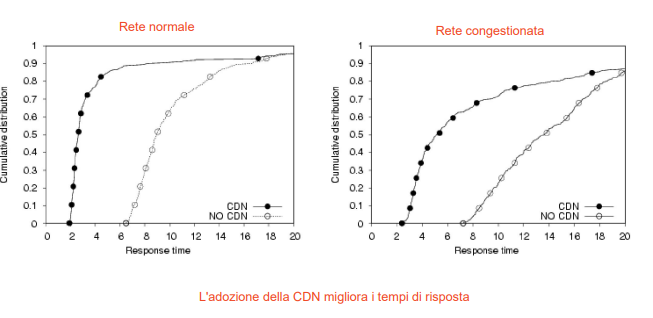
\includegraphics[width=0.8\textwidth]{SAC_A4_cdn.png}
		\end{figure}
		Nonostante le prestazioni migliorino con le CDN, la risoluzione del DNS è più complessa e richiede più tempo.
		\newpage
		
		\paragraph{Componenti CDN}
		La CDN usa delle tecniche di routing con algoritmi molto sofisticati per garantire che il client richiedente la risorsa venga instradato alla copia più vicina e nel modo più veloce possibile.
		Meccanismi per la gestione dei contenuti:
		\begin{itemize}
			\item URL Rewriting: La mappatura dei contenuti può essere basata sulla riscrittura delle pagine HTML. L'utente andrà a richiedere la pagina all'origin server che la CDN intercetterà e sovrascriverà gli embedded object con quelli presenti nella propria cache.
			\item DNS Outsourcing: Tramite questa tecnica è possibile evitare del tutto l'origin server grazie ai server DNS delle CDN. Tramite un meccanismo di risoluzione DNS intelligente è possibile, infatti, decidere se risolvere con l'IP dell'origin server o quello del server della CDN. Così facendo si può cachare sia la pagina che gli embedded object.
		\end{itemize}
		
		
		\begin{figure}[ht]
			\centering
			\begin{minipage}{0.5\textwidth}
				\centering
				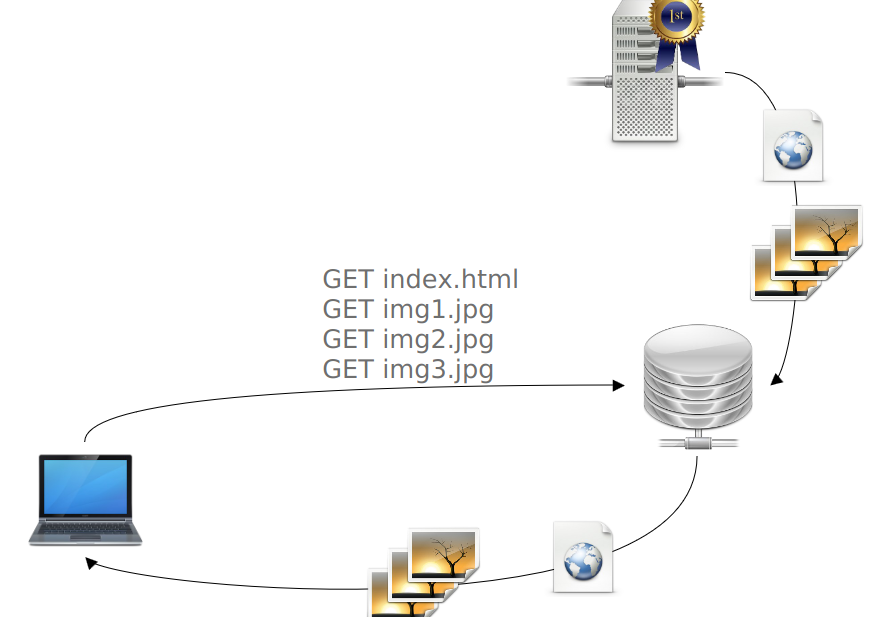
\includegraphics[width=0.9\linewidth]{images/SAC_A5_urlrewriting}
				\caption{URL Rewriting}
			\end{minipage}\hfill
			\begin{minipage}{0.5\textwidth}
				\centering
				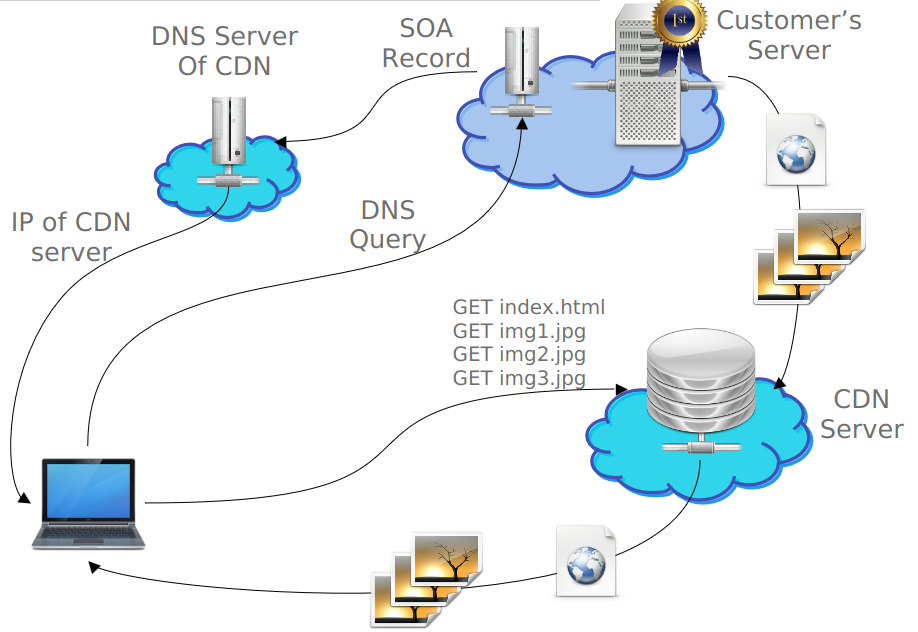
\includegraphics[width=0.9\linewidth]{images/SAC_A5_dnsoutsourcing}
				\caption{DNS Outsourcing}
			\end{minipage}
		\end{figure}

		
		Le soluzioni possono comunque essere mixate ad esempio tramite URL rewriting all'origin server e al primary CDN server mentre si potrebbe utilizzare il DNS outsourcing per bilanciare il carico tra origin, primary e secondary servers. 
		\newpage
		
		\section{Valutazione delle performance e simulazione}
		Vi sono due principali modi per fare performance evaluation: tramite modelli matematici e tramite
		simulazione.
		I primi sono in grado di rappresentare approssimativamente un sistema con le sue caratteristiche.
		Generalmente vengono utilizzati per fare una prima stima della complessità di un problema.
		I secondi, invece, permettono di simulare fedelmente o meno un sistema più complesso, poiché
		rappresentare un sistema di questo genere con modelli matematici inizia a diventare molto difficile.
		
		\begin{figure}[ht]
			\centering
			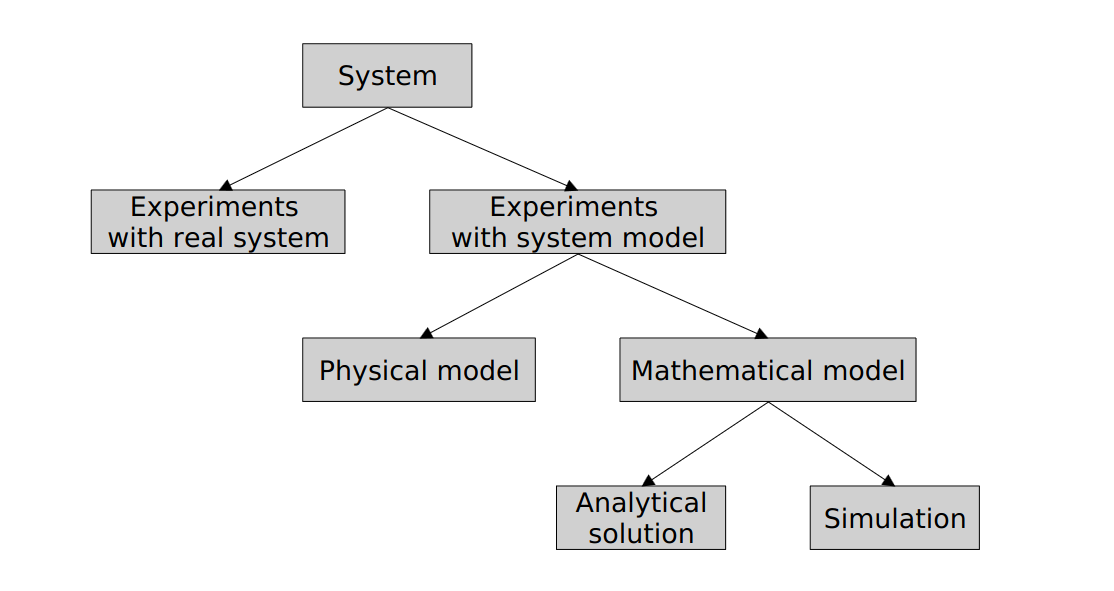
\includegraphics[width=0.7\linewidth]{SAC_D1_approaches}
			\label{fig:sacd1approaches}
		\end{figure}
		
		\begin{itemize}
			\item Esperimenti con sistemi reali: vengono fatti quando il sistema è molto semplice e contenuto. In questi casi si rivela più conveniente di altri approcci.
			\item Esperimenti con modelli del sistema complesso:
			\begin{itemize}
				\item Modelli fisici: sono rappresentazioni “in scala” del sistema stesso. Vengono tipicamente
				rappresentati tramite scenari virtualizzati. Generalmente sono più costosi degli altri tipi di
				modelli, inoltre rappresentare degli scenari “what if” è più difficile (cosa succede se il tempo
				di risposta è 100ms al posto che 50?)
				\item Modelli matematici: vengono utilizzati quando anche il modello fisico in scala è difficile da
				produrre. Per scenari “what if” è molto versatile, è molto facile trovare numeri anche
				approssimativi di scenari con carichi molto sbilanciati o molto alti, che magari sono difficili
				da rappresentare fisicamente. In linea teorica i modelli matematici sono i più
				accurati, ma necessitano di trovare il giusto livello di dettaglio
				\begin{itemize}
					\item Soluzioni analitiche: utilizzano modelli matematici per rappresentare il sistema tramite
					determinati costrutti matematici (generalmente variabili aleatorie). Uscire dai casi base
					del modello, tramite soluzioni analitiche, è molto più complesso però, quindi meno
					versatile
					\item Simulazione: tramite software è possibile simulare il comportamento di un sistema. È la via di mezzo fra modello matematico e modello reale, quindi un buon compromesso.
					Inoltre, è molto più versatile del modello matematico ma ha comunque degli intervalli di approssimazione di cui bisogna tenere conto
				\end{itemize}
			\end{itemize}
		\end{itemize}
		\newpage
		I parametri prestazionale di maggior interesse sono:
		
		\begin{itemize}
			\item Tempo di Risposta: intervallo fra accettazione di una richiesta e fine della risposta
			\item Throughput: volume di richieste soddisfatte nell'unità di tempo
			\item Error Rate: frazioni di richieste non servite correttamente
		\end{itemize}
		
		Tutti questi parametri dipendono direttamente dal carico corrente del sistema.\\
		
		Le classiche curve di carico di un sistema sono le seguenti:
		\begin{figure}[ht]
			\centering
			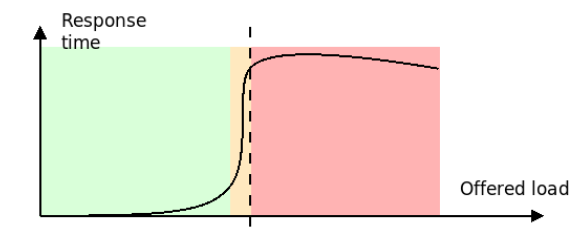
\includegraphics[width=0.7\linewidth]{SAC_D1_load1}
			\label{fig:sacd1load1}
		\end{figure}
		
		Il tempo di risposta varia in un modo preciso: rimane molto basso finché l’offered load (ovvero $\frac{richieste}{intervallo}$) rimane nella capacità del sistema. Quando si arriva a saturare il sistema si entra nella cosiddetta \textit{kneeling} zone, oltre la quale una piccola variazione di traffico fa variare di diversi ordini di grandezza il tempo di risposta.\\
		Ciò avviene non perché il sistema ci metta più tempo a processare le richieste bensì perché il traffico in arrivo, impossibile da processare, viene accodato.
		Più le code sono piene, più aumenta il tempo di risposta. Il limite superiore è garantito dal \textit{timeout} che impedisce alla curva di salire ancora. 
		
		\begin{figure}[ht]
			\centering
			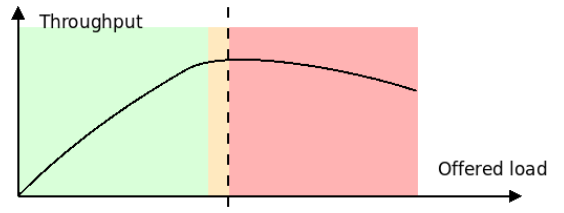
\includegraphics[width=0.7\linewidth]{SAC_D1_load2}
			\label{fig:sacd1load2}
		\end{figure}
		
		Il throughput invece cresce linearmente fino alla \textbf{saturazione}, momento nel quale raggiunge la capacità massima. Da quel punto in poi le richieste verranno accodate e il sistema passerà più tempo a gestire i context switch (\textit{trashing}) che ad eseguire lavoro utile. Il throughput quindi cala.
		
		\begin{figure}[ht]
			\centering
			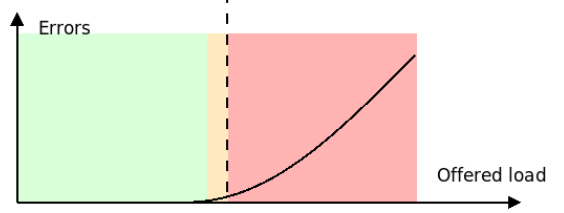
\includegraphics[width=0.7\linewidth]{SAC_D1_load3}
			\label{fig:sacd1load3}
		\end{figure}
		
		Conseguenza naturale dell’aumentare dei problemi di questo genere è l'aumento anche degli errori.
		L’obiettivo è quello di avere un sistema che si trovi in un intorno della fine della zona di sottoutilizzazione (quella verde): in questa zona il sistema non è né sottoutilizzato, né sovrautilizzato ma è al massimo della propria capacità tollerabile.
		L’ampiezza di questo intorno della kneeling zone dipende anche dal
		capacity planning che viene fatto, ovvero con che “lungimiranza”, rispetto alla quantità di traffico, viene costruito il sistema: quanto traffico in più è in grado di gestire il nostro sistema? Cosa succede se il traffico sale del 20\%? E del 30\%?
		
		
		\subsubsection{Modelli Basati su Sistemi a
			Coda}\label{modelli-basati-su-sistemi-a-coda}
		
		In questi modelli si considerano i sistemi a coda (con
		accodamento di richieste). Non serve che il modello ritorni un
		risultato preciso, è sufficiente conoscere almeno l'\emph{ordine di grandezza
			per sapere se è necessario scalare o meno}.
		
		\paragraph{Notazione dei Sistemi a Coda}\label{notazione-dei-sistemi-a-coda}
		I sistemi a coda vengono definiti mediante la seguente sintassi: \[
		\text{\{Processo di Arrivo\}/\{Processo di Servizio\}/Numero di Servitori/Lunghezza della Coda\}}
		\] Se la lunghezza della coda non viene specificata si assume che abbia
		lunghezza infinita. I Processi possono essere classificati con
		delle lettere, ciascuna corrispondente a una \emph{distribuzione di
			probabilità}:
		
		\begin{itemize}
			\tightlist
			\item
			M : Processo di Poisson (M sta per \emph{Memory
				Less}, caratterizzato dall'assenza memoria). Viene solitamente
			utilizzata per richieste non correlate tra loro, come
			ad esempio le sessioni utente.
			\item
			D : Processo Deterministico
			\item
			G: Processo Generico (solitamente Gaussiana o
			Log Normale, una Gaussiana con sopra un Logaritmico)
		\end{itemize}
		
		Un processo Poissoniano è un processo nel quale gli arrivi non dipendono dallo stato, ovvero la probabilità di un arrivo è indipendente dalle altre.
		\begin{itemize}
			\item Il tasso con cui arrivano i clienti è indicato con \(\lambda\)
			\item Il tasso con cui lasciano il sistema è indicato con \(\mu\)
			\item L'utilizzazione è indicata con \(\rho\) ed è uguale a \(\rho = \frac{\lambda}{\mu}\)
		\end{itemize}
		
		\paragraph{M/M/1}\label{mm1}
		Il tempo di risposta aumenta normalmente con l'aumento
		dell'utilizzazione (e quindi del carico) del sistema. Il \emph{tempo di
			risposta} \(T_R\) è dato da: \(T_R = \frac{1}{\mu-\lambda}\) .
		
		\paragraph{M/G/1}\label{mg1}
				
		In questi sistemi viene utilizzato il Teorema PASTA
		(Poisson Arrival See Time Average). Vengono introdotti diversi
		parametri come il tempo di attesa medio \(E[W]\), il
		tempo di risposta medio \(E[T]\) e il
		tempo medio di servizio \(E[S]=\frac{1}{\mu}\). In
		particolare, analizzando la formula del tempo di attesa medio, questo è
		dato da: \[
		E[W] = \frac{1+C_v^2}{2}+\frac{\rho}{1-\rho}
		\]
		Mentre il tempo medio di risposta è dato da:
		\[
		E[T] = 1+\frac{1+C_v^2}{2}\frac{\rho}{1-\rho}
		\]
		Dove \(C_v^2\) è il coefficiente di variazione,
		ovvero il \textbf{\emph{rapporto tra la deviazione standard e il valore
				medio}}, il quale \textbf{\emph{descrive la variazione del tempo di
				servizio}}. Per Poisson il valore di questo coefficiente è \(1\):
		trattandosi di sistemi senza memoria, questi tengono conto solo dello
		stato attuale del sistema.
		
			\paragraph{G/G/N}\label{ggn}
		Sistema Generico, senza restrizioni sul tipo di distribuzione dei
		processi di arrivo o di servizio. Anche il numero di servitori viene
		indicato con un numero \(n\) di servitori generici. Un sistema di questo
		tipo può essere usato per calcolare il tempo di risposta
		di un sistema generico.
		\[
		W_M = \frac{P_{cb,N}}{\mu N(1-\rho)}\frac{C^2_S+C^2_D}{2}
		\]
		\[
		P_cb,N \approx
		\begin{cases}
			(\rho^N+\rho) & \text{se $\rho \geq 0.7$}\\
			\rho^{\frac{N+1}{2}} & \text{otherwise}
		\end{cases}
		\]
		Segue l'approssimazione di Allen-Cuneen:
		\begin{itemize}
			\item $W_m$ = Tempo medio di attesa
			\item $P_cb,N$ = Probabilità che tutti i server siano impegnati.
			\item $C_s, C_d$ Coefficiente di variazione(deviazione standard / media):
			\begin{itemize}
				\item $C_s$: Arrivo
				\item $C_d$: Servizio.
			\end{itemize}
		\end{itemize}
		
		\subsubsection{Metriche di Failure}\label{metriche-di-failure}
		\begin{quote}
			MTBF: Mean Time Between Failures \\
			MTTF: Mean Time To Failures \\
			MTTF: Mean Time To Repair
			
			\(MTBF = MTTF + MTTR\)
		\end{quote}
		
		La disponibilità \(A\) (Availability) è data da: \[
		A = \frac{MTTF}{MTBF} = 1 - \frac{MTTR}{MTBF}
		\] Sulla base di questo fattore è possibile calcolare delle
		classi di disponibilità.\\
		
		La replicazione geografica può essere talvolta un metodo di \textbf{\emph{autoriparazione dei problemi senza personale}}. Nei sistemi come i datacenter la recovery in seguito a un guasto deve essere
		fatta automaticamente, mentre il rilevamento degli errori può essere fatto
		durante il funzionamento del sistema (\emph{concurrent detection}) o nei \textbf{\emph{momenti in cui le operazioni sono	sospese}} (preemptive detection).
		
		
		Considerando invece \(N\) sottosistemi, ciascuno con una
		probabilità di failure \(r_i\) la \textbf{probabilità
			che fallisca l'intero sistema} \(R\) dipende dalla
		tipologia di interazione del sistema:
		
		\begin{itemize}
			\tightlist
			\item
			Seriale: basta che un solo sottosistema fallisca →
			\(R=\prod r_i\)
			\item
			Parallelo: tutti i sottosistemi devono fallire
			→~\(R = 1- \prod (1-r_i)\)
		\end{itemize}
		
		\subsubsection{CAP Teorem}\label{cap-teorem}
		
		Il CAP Teorem afferma che nella \emph{progettazione di un
			datacenter} è possibile scegliere solo \textbf{\emph{due
				caratteristiche}} tra:
			\begin{itemize}
				\item Consistency: ogni client vede lo stesso dato anche dopo una modifica o una cancellazione
				\item Availability: ogni client può trovare una replica del dato anche in caso di fallimenti parziali dei nodi
				\item Partition Tolerance: il sistema continua a funzionare nonostante malfunzionamenti parziali
			\end{itemize}
		
		\newpage
		\section{Modelli di costo}
		Esistono vari modelli di business per il cloud computing:
		\begin{itemize}
			\item Servizi: Vendere le proprie competenze.
			\item Prodotti: Creare e vendere i propri prodotti (Software).
			\item Vendita: Vendere prodotti di terze parti.
		\end{itemize}
		
		\subsection{Servizi}
		Necessita di un basso costo di setup iniziale, ma bisogna conoscere bene il modello di business. Il successo è determinato dall'introduzione di qualcosa diverso da ciò già presente nel mercato da un punto di vista di qualità, competenze o prezzi.
		Il business richiede un dispendio di risorse umane ad alta intensità, non è scalabile come un prodotto. E' importante saper gestire le relazioni con i clienti, in quanto il lavoro spesso tende a compiacere quest'ultimo e i vincoli da lui imposti, che possono anche limitare la creatività del prodotto.
		Il mercato del cloud è basato sulla fiducia e la reputazione dato che i clienti spesso non hanno le competenze per valutare il servizio e si basano sulle reputazioni.
		
		\subsection{Prodotto}
		Ci si aspetta di ricavare grandi quantità di denaro in tempi ricorrenti, tuttavia la realtà è ben diversa in quanto i software e i prototipi non sono dei veri e propri prodotti ma bisogna cercare di indovinare i futuri bisogni dei clienti. 
		Spesso si lavora su qualcosa senza alcuna garanzia di ritorno, incorrendo anche nel fallimento nei casi peggiori. Costruire un nuovo prodotto può essere dispendioso sia da un punto di vista economico che psicologico.
		Da un punto di vista finanziario si avranno degli alti e bassi, infatti la fatturazione è basata sul tempo.\\
		Possiamo individuare due categorie di costi:
		\begin{itemize}
			\item CAPEX: Ammortizzati durante gli anni. Ci danno una riduzione del flusso di cassa disponibile
			\item OPEX: Fondi per gestire le attività quotidiane, si esauriscono entro l'anno di acquisto
		\end{itemize}
		
		\subsubsection{Metriche di costi}
		\paragraph{TCO} \mbox{}\\
		
		\begin{figure}[ht]
			\centering
			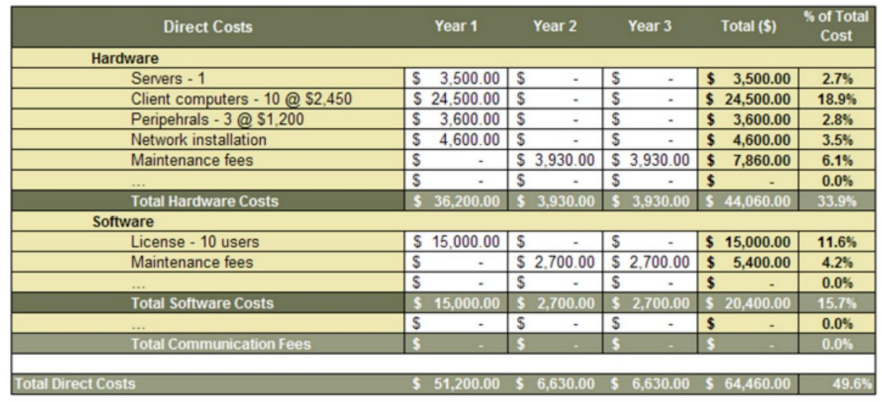
\includegraphics[width=0.8\textwidth]{SAC_D1_TCOExample.png}
		\end{figure}
		Costo totale di proprietà, tutti i costi diretti, CAPEX, e indiretti, OPEX, di gestione di un bene durante la sua vita utile.\\
		Le spese in conto capitale (CAPEX) sono spese per l'acquisto di beni o servizi significativi che verranno utilizzati per migliorare le prestazioni dell'azienda in futuro. Le spese in conto capitale riguardano tipicamente attività fisse come immobili, impianti e attrezzature (PP\&E). Questi costi vengono ammortizzati nel corso degli anni.\\
		Le spese operative (OPEX) sono i costi che un'azienda sostiene per la gestione delle sue attività quotidiane. In quanto tali, non si applicano ai costi relativi alla produzione di beni e servizi. Tipicamente riguardano gli acquisti per i consumi entro l'anno di attività.\\
		
		Per calcolare il TCO, bisogna valutare le spese di hardware e software, il supporto gestionale e tecnico, tempo di formazione, eventuali viaggio e contratti di supporto, implementazione e costi di comunicazione.
		
		
		\paragraph{Vantaggi TCO}
		Rappresenta non solo l'investimento iniziale ma considera anche tutti gli altri costi associati. Assicura un'analisi completa a lungo tempo.
		
		\paragraph{Svantaggi TCO}
		Non considera i vantaggi delle varie opzioni non considerate, non da nessuna tempistica e comporta un costo di acquisizione elevato. Inoltre può essere difficile quantificare tutto.
		Per un'azienda considerare un TCO significa seguire una strategia basata sul costo minimo piuttosto che sul massimo rendimento.
		
		\paragraph{ROI}\mbox{}\\
		Il ritorno sull'investimento ha lo scopo di confrontare i costi di un progetto con il valore dei suoi risultati, viene espresso in percentuale di un periodo: $$ ROI =\frac{Utile Netto}{ Investimento} * 100 $$
		Grazie a questo modello siamo in grado di analizzare la tempistica e l'entità degli investimenti, oltre che a considerare più scenari.
		Gli errori più comuni si verificano quando si sottovalutano gli investimenti o non si tiene conto del tempo impiegato dai dipendenti o del costo del capitale nel tempo.\\ 
		
		Esempio:\\
		\begin{quote}
		Costi totali: 114.000 €\\
		Guadagni totali: 180.000 € / anno\\
		ROI: 66.000 / 114.000 € * 100 = 57.8%
		\end{quote}
		
		\newpage
		\section{Virtualization}
		Vi sono diversi motivi per utilizzare la virtualizzazione nel cloud:
		\begin{itemize}
		    \item Ridurre l'utilizzo dell'hardware consolidando i server
		    \begin{itemize}
		        \item Indipendenza Hardware.
		        \item Migliore scalabilità.
		        \item Gestione semplificata.
		    \end{itemize}
		    \item Continuità
		    \begin{itemize}
		        \item Backup
		        \item Ripristino di emergenza
		        \item Alta disponibilità
		        \item Failover hardware (multipathing)
		    \end{itemize}
		    \item Maggiore efficienza nella gestione del ciclo di vita del software (sviluppo e test)
		    \begin{itemize}
		        \item Ambiente di test
		        \item Provisioning delle applicazioni
		        \item Switch semplificato tra le versioni del software
		    \end{itemize}
		\end{itemize}
		
		\emph{Definizione} La virtualizzazione è: 
		\begin{quote}
			Astrazione delle componenti hardware degli elaboratori col fine di fornirli al software sotto forma di risorsa virtuale.
		\end{quote}
		Possibili oggetti di virtualizzazione:
		\begin{itemize}
		    \item Risorse hardware (es, CPU, GPU, memoria)
		    \item Risorse di archiviazione 
		    \item Risorse di rete
		\end{itemize}
		La virtualizzazione è una tecnologia abilitante per il Cloud, come mostrato nel modello IaaS dove si usano VMs per astrarre problemi hardware.\\
		
		La virtualizzazione può avvenire a diversi livelli:
		\begin{itemize}
			\item Emulazione \textrightarrow  Circuiti
		    \item Virtualizzazione \textrightarrow  Hardware
		    \item Containerizzazione \textrightarrow  Sistema operativo
		\end{itemize}
		
		\subsection{Emulazione}
		Emulazione di componenti hardware che tipicamente hanno un'architettura differente da quella dell'host, per cui occorre tradurre le operazioni macchina generate dal processore nell'architettura di destinazione. Presenta un'ottima flessibilità nonostante il grande overhead.\newline
		Esempi:
		\begin{itemize}
		    \item  BOCH
		    \item  VICE (Commodore 64 emulator)
		\end{itemize}
		
		\subsection{Virtualizzazione}
		Terminologia:
		\begin{itemize}
		    \item Hypervisor: software per l'esecuzione di VM
		    \item Virtual Machine (VM) 
		    \item Guest: Una VM
		    \item Host: il calcolatore in cui viene fatto girare l'hypervisor
		\end{itemize}
		Ogni Guest vede le proprie risorse hardware, le quali sono state virtualizzate a partire dall'hardware presente sull'host, senza accorgersi della virtualizzazione. Più VM possono esistere sullo stesso Host e possono lanciare sistemi operativi diversi e combinazioni di hardware differenti.\\
		Alcuni esempi:
		\begin{itemize}
		    \item VMWare
		    \item VirtualBox
		    \item Xen
		    \item KVM
		\end{itemize}
		
		\paragraph{Containerizzazione}
		Più ambienti separati:
		\begin{itemize}
		    \item Gruppo di processi per ogni ambiente (es. \verb*|cgroups|)
		    \item Separazione tra gruppi di processi (es. \verb*|namespace|)
		\end{itemize}  
		Tutti i gruppi di processi condividono lo stesso kernel, tipicamente Linux. Sono presenti software aggiuntivi per la gestione: delle immagini del file-system, della rete o del ciclo di vita dei container.\newline
		Esempi:
		\begin{itemize}
		    \item Docker
		    \item Kubernetes (Google)
		\end{itemize}
		
		\subsection{Approccio alla virtualizzazione}
		Grazie alle definizioni di macchina virtuale, memoria virtuale e hypervisor, possiamo definire alcuni concetti che forniscono i requisiti minimi hardware per supportare la virtualizzazione.\\
		
		Un primo approccio storicamente utilizzato è "\emph{Trap ed execute}": il codice gira sul guest fino a quando non viene invocata una istruzione \textbf{sensibile} che genererà una trap. Le trap sono gestite dall'hypervisor che si occupa di emulare il comportamento corretto e far riprendere l'esecuzione.
		
		\begin{figure}[ht]
			\centering
			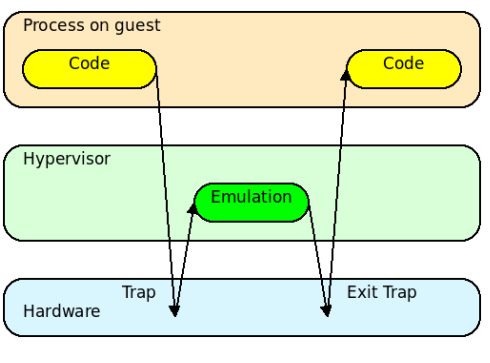
\includegraphics[width=0.4\textwidth]{SAC_B1_hypervisorTrap.png}
		\end{figure}
		
		Come si può notare, non tutte le istruzioni sono uguali, infatti quelle che possono accedere o modificare lo stato della macchina vengono considerate critiche in quanto possono:
		\begin{itemize}
		    \item Interrompere l'esecuzione.
		    \item Accedere al registro degli stati.
		    \item Accedere alla memoria tramite indirizzo fisico.
		\end{itemize}
		Le istruzioni sensibili devono quindi essere gestite solo dall'hypervisor tramite l'uso di "trap" a livello hardware.\\
		
		Queste operazioni di trap sono onerose e rendevano lente le piattaforme virtuali, ecco perchè la virtualizzazione ha cominciato a perdere d'interesse. Le tecnologie abilitanti per il cloud computing hanno fatto si che la virtualizzazioni prendesse più piede tra le tecnologie emergenti degli ultimi anni. Il nuovo approccio consiste nell'utilizzare software appositamente ottimizzato per la virtualizzazione e l'introduzione di supporto hardware compatibile con quest'ultima e notevolmente più potente. 
		
		\subsection{Principi di virtualizzazione}
		Grazie al paper di Popek e Goldberg del 1974 si stabilirono delle basi teoriche sui concetti chiave e requisiti della virtualizzazione, oltre che alla definizione dell'approccio trap and execute.\\
		\emph{Definizione} VM: 
		\begin{quote}
			Una macchina virtuale è considerata un duplicato efficiente e isolato della macchina reale.
		\end{quote}
		Come software un VMM ha tre caratteristiche essenziali. In primo luogo, il VMM fornisce un ambiente per i programmi che è essenzialmente identico al computer originale; secondo, i programmi eseguiti in questo ambiente mostrano nel peggiore dei casi solo lievi diminuzioni di velocità; e infine, il VMM ha il controllo completo delle risorse di sistema.\\
		
		Identifichiamo quindi tre requisiti fondamentali:
		\begin{itemize}
			\item Equivalence/Fidelty
			\item Resource control/Safety
			\item Efficiency/Performance
		\end{itemize}
		E una differente classificazione delle istruzioni:
		\begin{itemize}
		    \item Istruzioni \textbf{sicure}: Eseguibili dal guest senza problemi
		    \item Istruzioni \textbf{privilegiate}: Supponendo che la CPU abbia due modalità di esecuzione, supervisor (\textit{ring 0}) e standard (\textit{ring 3}), queste istruzioni sono eseguibili solo in modalità supervisor.
		    \item Istruzioni \textbf{sensibili}: Sono quelle istruzioni che l'hypervisor deve trappare per emulare il normale comportamento di un OS dando l'illusione al guest di possedere le risorse hardware
		\end{itemize}
		Se tutte le istruzioni sensibili sono anche privilegiate, la virtualizzazione diventa più facile e i trap vengono generati automaticamente quando un'istruzione sensibile viene eseguita dall'hypervisor. Se invece sono presenti istruzioni sensibili che non sono privilegiate potremmo avere dei problemi, in quanto l'hypervisor non può fare affidamento su trappole per acquisire e modificare il proprio comportamento e diventa più complessa l'implementazione. 
		
		\newpage
		\subsection{Tecniche di virtualizzazione}
		Abbiamo visto precedentemente che le tecniche virtualizzazione si basano sul livello al quale vogliamo eseguire l'astrazione (emulazione, virtualizzazione, container), 
		attraverso approcci basati sull'hardware o sull'approccio per gestire le istruzioni sensibili (Trap and execute, traduzione binaria, patch binaria)
		\begin{figure}[ht]
		    \centering
		    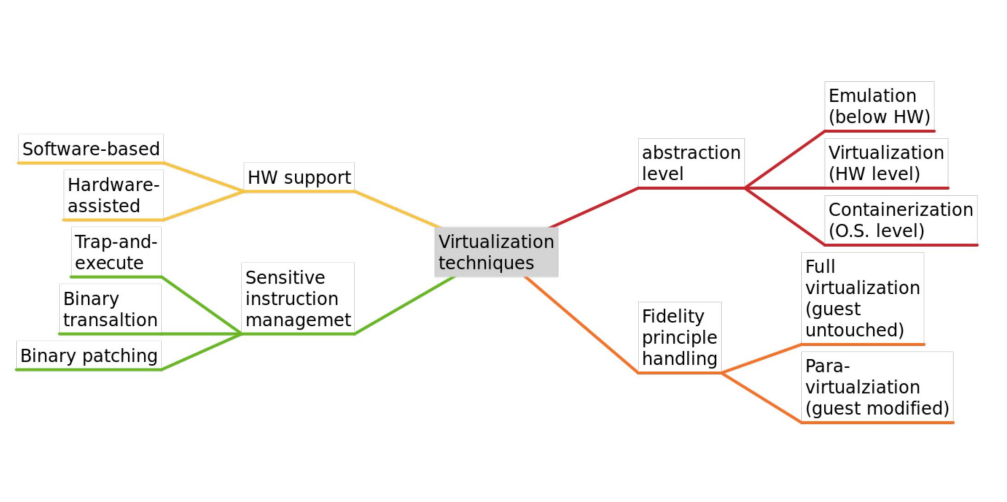
\includegraphics[width=0.6\textwidth]{SAC_B1_virtualizationTechnicques.png}
		\end{figure}
		
		\subsubsection{Emulazione}
		Attraverso un interprete emula il comportamento dell'hardware riproducendo l'architettura emulata. Il sistema operativo nativo viene eseguito sull'hardware emulato riproducendo le caratteristiche principali del chip. 
		\begin{itemize}
		    \item Vantaggi:
		    \begin{itemize}
		        \item Separazione completa dall'ambiente emulato.
		        \item Può eseguire software per hardware diverso.
		        \item Elevata flessibilità.
		    \end{itemize}
		    \item Svantaggi:
		    \begin{itemize}
		        \item Enorme overhead
		        \item Non è per nulla vicino alla velocità nativa a meno che non si emuli un hardware più vecchio.
		    \end{itemize}
		\end{itemize}
		
		\subsubsection{Traduzione binaria}
		A differenza dell'approccio basato sulle trap, che funziona a \textit{tempo di esecuzione}, viene effettuato un cambio di paradigma passando ad un approccio proattivo intervenendo sul codice prima che questo venga eseguito. 
		Grazie alla compilazione anticipata, introdotto per dare supporto all'emulazione, questo metodo viene usato anche adesso nei sistemi di virtualizzazione.\\
		I suoi punti cardine sono:
		\begin{itemize}
		    \item La traduzioni di istruzioni sensibili ma non privilegiate.
		    \item Può funzionare anche in fase di esecuzione.
		    \item Può memorizzare nella cache il codice tradotto. 
		\end{itemize}
		Principalmente si hanno due compiti:
		\begin{itemize}
		    \item Scansione del codice: Viene analizzata solo una porzione del codice, concentrandosi a livello kernel, lasciando in sicurezza il codice \emph{userspace} perché si presuppone che quest'ultimo non utilizzi funzioni sensibili.
		    \item Modifica del codice: Viene modificato il codice delle istruzioni sensibili in codice sicuro, \textbf{mantenendo} entrambe le copie.
		\end{itemize}
		Le unità di codice considerate sono sequenze di istruzioni denominate basic block.
		I blocchi possono essere tradotti una volta, riscrivendo gli indirizzi di salto presenti nel codice originale, e salvati nella cache per un eventuale riutilizzo.
		\begin{figure}[ht]
		    \centering
		    \begin{minipage}{0.5\textwidth}
		        \centering
		        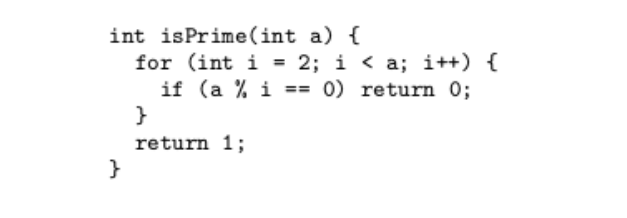
\includegraphics[width=0.9\textwidth]{SAC_B1_binaryTranslation01.png} % first figure itself
		        \caption{Codice in C}
		    \end{minipage}\hfill
		    \begin{minipage}{0.5\textwidth}
		        \centering
		        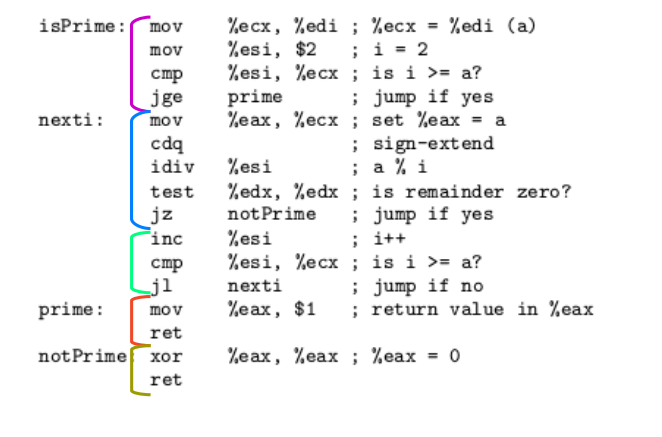
\includegraphics[width=0.9\textwidth]{SAC_B1_binaryTranslation02.png} % second figure itself
		        \caption{Codice del compilatore tradotto}
		    \end{minipage}
		\end{figure}
		\newpage
		Regole per la traduzione:
		\begin{itemize}
		    \item IDENT: il codice può essere tradotto in modo identico
		    \item Flusso di controllo diretto: Mappatura degli indirizzi in codice tradotto per istruzioni jmp, call, ret
		    \item Flusso di controllo indiretto: Quando l'indirizzo non è disponibile al momento della traduzione bisogna calcolare gli indirizzi al volo.
		    \item Istruzioni privilegiate: Bisogna riscriverle accuratamente
		\end{itemize}
		La traduzione binaria riduce l'overhead durante l'esecuzione in quanto il grosso del compito viene svolto prima dell'esecuzione del programma, in fase di compilazione. 
		
		\subsubsection{Patch Binaria}
		E' molto simile alla traduzione binaria ma la differenza sta nella gestione del codice tradotto.
		In questo caso il codice tradotto va a Una macchina virtuale è considerata un duplicato efficiente e isolato della macchina reale. il codice originale. Inoltre il controllo per la memorizzazione della cache è più complesso.
		Un esempio di questa tecnica di virtualizzazione è Virtual Box
		
		\subsubsection{Paravirtualizzazione}
		Il software di paravirtualizzazione agisce direttamente sull'hardware in modo da gestire la condivisione delle risorse destinate alle varie virtual machine.
		Il codice del guest quando deve eseguire istruzioni sensibili utilizza delle API per interagire con l'hypervisor per interrupt o paginazione della memoria, dette \textbf{hypercalls}.
		Come nel caso della traduzione binaria, la traduzione avviene in fase di compilazione.
		L'esempio più comune è il progetto Xen.\\ 
		
		\begin{figure}[ht]
			\centering
			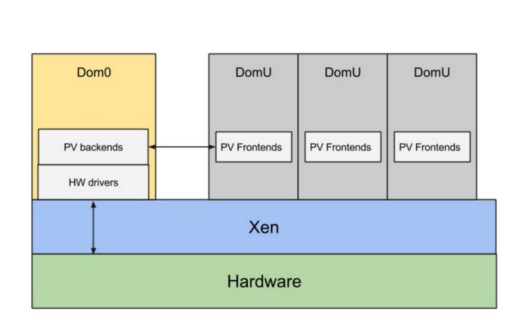
\includegraphics[width=0.6\textwidth]{SAC_B1_virtualizationIO_Par.png} % second figure itself
		\end{figure}
		
		I limiti sono:
		\begin{itemize}
		    \item Modificare il guest: Occorre il supporto da parte del sistema operativo.
		    \item Per rappresentare una valida alternativa deve essere integrata con altre opzioni quando non è possibile modificare il guest.
		\end{itemize}
		Tramite la paravirtualizzazione è possibile caricare un device driver (\emph{dom0}) che è conscio di
		essere all’interno di un ambiente virtualizzato. In questo modo è possibile creare una
		periferica \textit{dummy} che non fa nient’altro che scrivere su un buffer di memoria che verrà successivamente
		letto da dom0 (tramite hypercall). Una volta fatto ciò il device driver si occuperà, infine, di comunicare effettivamente con l'hardware.\\ 
		
		\begin{figure}[ht]
			\centering
			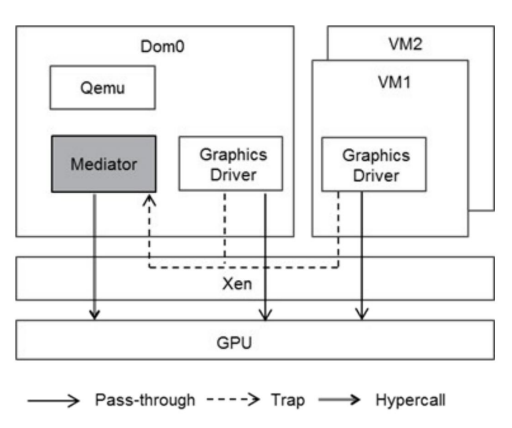
\includegraphics[width=0.6\textwidth]{SAC_B1_virtualizationIO_PCI.png} % second figure itself
		\end{figure}
		
		Inoltre, la gestione della memoria viene fatta in maniera più ottimizzata: dom0 (o
		equivalenti) genera un processo che cerca di occupare quanta più RAM libera possibile
		così da facilitare il lavoro dell'hypervisor quando dovrà assegnarla. In questo modo non c’è
		bisogno di tradurre la RAM vera con quella del guest stesso (come avviene in
		ambienti virtualizzati canonici).
		
		\paragraph{Gestione dell'hardware}
		Sono concetti implementati sia in hypervisor di virtualizzatori completi sia in hypervisor di para virtualizzatori.
		\begin{itemize}
		    \item Emulazione dell'hardware: Massimizza la sicurezza. Utilizza la tecnica trap and execute. Si può avere un enorme overhead portando a un basso throughput e pessime performance per i video. 
		    \item Accesso diretto all'hardware: Per i dispositivi che lo supportano è possibile assegnarli direttamente alla macchina virtuale. Massimizza le performance a discapito della sicurezza. Un ruolo importante dell'hypervisor è quello di escludere l'accesso simultaneo allo stesso hardware.
		    \item Split driver: Un compromesso tra i due. In questo caso si hanno due parti:
		    \begin{figure}[ht]
		    	\centering
		    	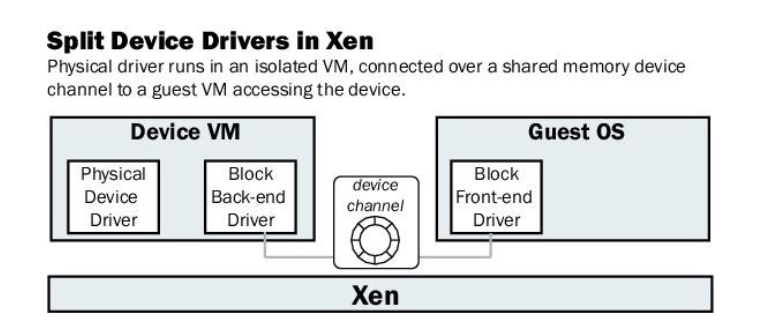
\includegraphics[width=0.7\linewidth]{images/SAC_B1_splitdriver}
		    	\label{fig:sacb1splitdriver}
		    \end{figure}
		    \begin{itemize}
		        \item Back-end che può accedere all'hardware e gestisce l'accesso simultaneo. Si occupa di fare l'accesso all'hardware.
		        \item Front-end che è in esecuzione sul guest, non è altro che una coda di richieste da cui il backend preleverà.
		    \end{itemize}
		    
		    Back-end e Front-end sono consapevoli l'uno dell'altro e scambiando dati in modo efficiente usando hypercall e code di eventi.
		    Esempio: VmWare.
		\end{itemize}
		
		\subsection{Extensions}
		\paragraph{Memory Ballooning}
		Questo metodo viene utilizzato per gestire la RAM in maniera efficiente. Spesso, le
		macchine virtuali non utilizzano tutta la RAM a loro assegnata, pertanto viene usato un
		processo “\emph{ballooner}” per occupare le pagine di memoria correntemente non utilizzate, "gonfiandosi".\\
		Quando una VM richiederà più RAM, l’hypervisor potrà interrogare il
		ballooner per richiedere la memoria da assegnare alla VM, facendolo "sgonfiare". Grazie alla delega di queste operazioni, l'hypervisor può essere meno complesso in termini di codice.\\
		
		Anche una live migration di una macchina virtuale potrà essere molto più efficiente da
		implementare, poiché le pagine non utilizzate dalla macchina virtuale sono ancora
		assegnate al ballooner e non alla macchina virtuale, risparmiando notevolmente tempo.
		
		\paragraph{Estensioni Hardware}
		Per soddisfare i requisiti di P\&G, le architetture vengono estese per avere un ulteriore
		livello destinato all'hypervisor di operatività (\emph{ring -1}). Ci sono quindi istruzioni in più che gli hypervisor
		possono utilizzare per funzionare. Queste funzioni non sono solo di interesse della
		CPU, ma anche per varie periferiche I/O, oltre che alla RAM.
		Per quanto riguarda Intel, sono disponibili tre estensioni: CPU, IOMMU (I/O e RAM) e
		network.
		
		\begin{figure}[ht]
			\centering
			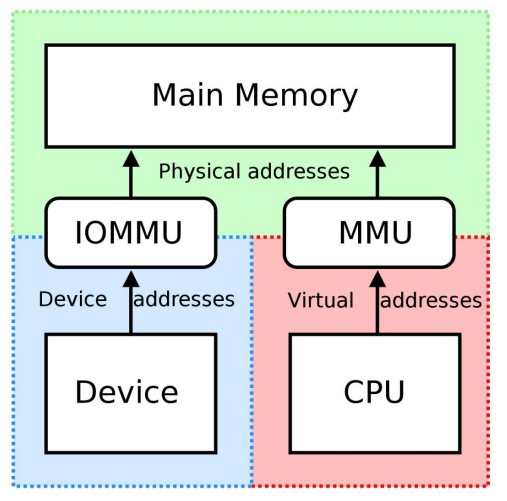
\includegraphics[width=0.4\textwidth]{SAC_B1_virtualizationIO_HW.png} % second figure itself
		\end{figure}
		
		Vengono aggiunte quindi 10 nuove istruzioni adibite a questo; inoltre, vengono aggiunte
		altre due modalità di operazione (all’interno della modalità hypervisor), VMX root e VMX
		non-root, usato dalle macchine guest.\\
		In realtà quello che avviene è che il numero di modalità raddoppiano: vi sono 4 rings per
		VMX non-root e altrettanti per VMX root, per emulare completamente tutto lo stack.
		Questo significa che, ad esempio, il kernel di una macchina guest girerà al
		\emph{ring 0} VMX non-root mentre il kernel dell’hypervisor girerà a \emph{ring 0} VMX root. Per commutare 
		modalità verranno utilizzate apposite traps.\\
		
		Vengono anche create delle strutture dati (VM control structures) che
		permettono di gestire le macchine virtuali come se fossero dei processi (come i \textit{Process Control Blocks}).
		Le istruzioni aggiuntive permettono di
		interagire con tali strutture dati, consentendo di gestire le macchine virtuali a
		livello hardware.
		
		\paragraph{Estensioni Network and I/O}
		In questo caso, il problema è quello di andare ad accelerare le operazioni di I/O con
		supporto hardware. Ad esempio, avendo una scheda di rete prestante, il sistema
		operativo ha accesso diretto alla periferica (DMA). È possibile fare la stessa cosa in un
		contesto virtualizzato? Sì, infatti è possibile rimappare la gestione della memoria da
		parte dell’hypervisor in modo tale che le macchine guest possano utilizzare il supporto
		hardware per questo genere di cose.
		
		\subsection{Virtualizzazione della memoria}
		Nel contesto virtualizzato, il modello paginato inizia ad avere dei problemi, serve un livello
		di indirettezza ulteriore.
		Tipicamente è possibile risalire alle pagine fisiche, partendo da quelle logiche, semplicemente consultando la \emph{page table}. In un contesto virtualizzato occorre, però, una page table su più livelli: uno per la macchina virtuale, che sta sull’host, e
		uno per ogni macchina virtuale e i suoi spazi di indirizzamento.\\
		
		La virtualizzazione aggiunge quindi anche un altro livello indiretto: per ogni guest sono presenti pagine fisiche che fisiche non sono perché l'hardware è virtualizzato. Vengono dunque sviluppati, dai vendor
		delle CPU, supporti hardware per TLB \emph{innestata} e la MMU.
		\begin{figure}[ht]
			\centering
			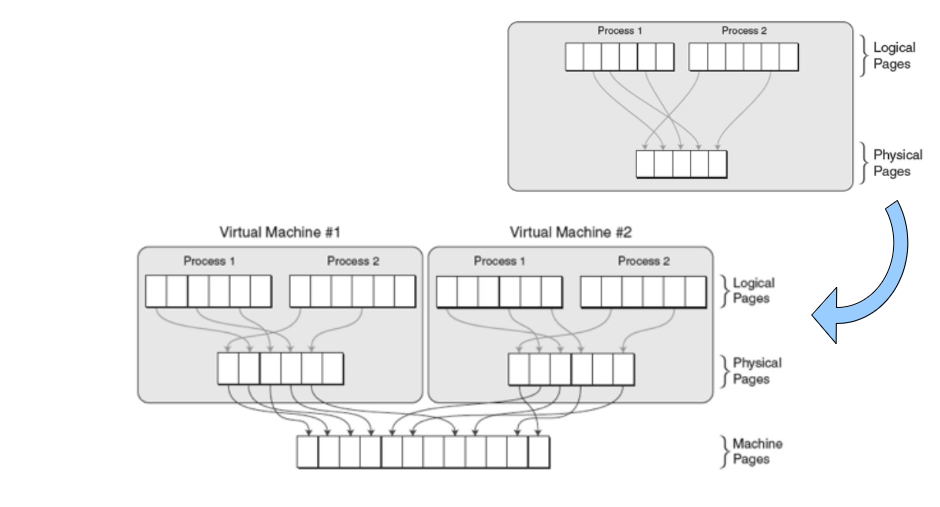
\includegraphics[width=0.7\linewidth]{images/SAC_B5_nestedtlb}
			\label{fig:sacb5nestedtlb}
		\end{figure}
		
		Tuttavia, è necessario che a partire dalla page table guest non sia possibile risalire fino a quella fisica dell'host, altrimenti il guest avrebbe essenzialmente il controllo della macchina. Vengono in aiuto le cosiddette \textbf{shadow page tables}, tabelle costruite dall'hypervisor, in cui si tiene traccia della rappresentazione delle page table del guest. Viene utilizzato il registro \verb*|CR3|, un puntatore al base page register per il guest correntemente in esecuzione, per gestire il cambio di page table.\\
		La necessità di mappare le operazioni sulle pagine guest alle pagine dell'host può però portare ad un sovraccarico significativo nonostante sia trasparente per i guest.\\ 
		
		Un approccio alternativo prevede l'uso della paravirtualizzazione: guest e VMM condividono le tabelle ma il guest ha accesso in sola lettura alle pagine e la modifica avviene per mezzo di hypercall.
		Questo approccio particolarmente efficiente è utilizzato in Xen.\\
		
		L'approccio attuale prevede invece l'utilizzo delle pagine nidificate, affidandosi al supporto hardware. Vi è un TLB per le pagine dei guest e uno aggiuntivo per mappare l'indirizzo fisico sull'host.
		

		\subsection{Virtualizzazione dell'archiviazione}
		Un grosso problema delle macchine virtuali è la rappresentazione dei loro dischi.
		Generalmente, lo spazio di indirizzamento di un disco è un blocco di dati identificato
		da una terna di dati: 
		\begin{itemize}
			\item Settore
			\item Distanza della testina dal centro
			\item Piatto
		\end{itemize}
		La rappresentazione di un disco fisico deve essere mappata in un qualche modo su un file. Abbiamo due possibili approcci:
		\begin{itemize}
		    \item VMDK: Consiste nella descrizione di un'immagine del disco fisica rappresentante la geometria e i settori del disco. La struttura del file è \textbf{sparsa}, cioè i blocchi vuoti non occupano effettivamente spazio ma se ne tiene traccia tramite metadati, così da ottimizzare lo spazio su disco. L'altra rappresentazione è quella \textbf{flat}, cioè l'allocazione contigua del file.\\ 
		    
		    I file VMDK permettono di creare degli \textbf{snapshot} dei filesystem: una volta che ho, ad
		    esempio, installato il sistema operativo è possibile catturare un'istantanea dello stesso.
		    Viene quindi creato un nuovo layer sul quale verranno scritte le modifiche successive. Per realizzare questo meccanismo vengono usati i
		    \textit{delta links}, che contengono le modifiche fatte sullo snapshot (\textbf{base disk}).\\
		    Diverse copie della stessa VM potranno partire dalla stessa immagine di base per creare diverse versioni con le proprie modifiche apportate mediante i delta links.
		    \item QCOW: Evolve VMDK, implementando compressione, crittografia. Aggiunge support a sparse files anche se il sistema operativo host non lo supporta.
		    \item File Docker a più livelli, come squashFS.
		\end{itemize}
		
		\subsection{Gestione delle risorse}
		La prima risorsa da dover gestire accuratamente è la memoria che deve essere sempre allocata e restituita all'hypervisor quando non viene utilizzata dal guest.\\
		
		Per quanto invece riguarda la CPU, per evitare che le macchine virtuali la saturino è necessario un intervento dell'hypervisor che fissa un limite agli utilizzi delle varie VM. 
		Lo \textit{stealing} della CPU si verifica quando i processi sono pronti per essere eseguiti dalla CPU virtuale ma rimangono in attesa che l'hypervisor assegni loro una CPU fisica. Ciò accade perché l'hypervisor sta servendo un'altra macchina virtuale.
		Se $steal > 0$ l'hypervisor deve applicare il limite.
		Ci sono due cause principali di \emph{steal} della CPU:
		\begin{itemize}
		    \item I processi richiedono più della CPU a loro allocata
		    \item Il server fisico è sovraccaricato dalle macchine virtuali
		\end{itemize}
		Sfortunatamente, è difficile capire in quale di questi due casi rientra una situazione solo guardando lo \emph{stealing time}.\\
		
		L'ultimo problema da gestire è l'\textbf{interferenza} tra le varie macchine virtuali, ovvero la contesa sulle risorse (CPU, Rete) fisiche. Ad esempio ogni volta che avviene un context switch tra VM la cache si svuota per accogliere i contenuti del nuovo guest. E' difficile ottenere un perfetto isolamento delle prestazioni tra varie macchine virtuali anche se di norma il comportamento di una macchina virtuale non dovrebbe infierire su altre macchine virtuali.\\
		Una conseguenza di questo fenomeno è il fatto che le interferenze possano essere usate come \emph{side-channel} per attacchi informatici: due macchine virtuali apparentemente non comunicanti tra di loro, possono in realtà interagire facendo appositamente variare l’utilizzo di risorse. Questa variazione può essere codificata per comunicare oppure ottenere informazioni dalle altre VM.
		
		\subsection{Migrazioni di macchine virtuali}
		Può succedere che sia necessario migrare una macchina da un nodo all’altro. Gli scenari possibili sono:
		\begin{itemize}
			\item Migrazione offline: stop su nodo 1 e restart su nodo 2
			\item Live migration: migrazione senza downtime da nodo 1 a nodo 2
		\end{itemize}
		La migrazione offline è il tipo di migrazione più facile da implementare per un
		hypervisor, ma non necessariamente quella ideale in scenari di high availability.
		
		\paragraph{Live Migration}
		La live migration è più complessa e viene generalmente implementata tramite il processo di pre-copy, che ha quattro fasi: preparation, memory copy, migration, resume.
		\begin{itemize}
			\item Preparation: si fa uno snapshot del disco con layer multipli per facilitarne il
			trasferimento
			\item Memory copy: dato il principio di località, una macchina virtuale avrà una lista di
			“hot pages” che starà accedendo. Generalmente, l’hypevisor durante questo step
			ha già creato la macchina di destinazione e inizierà a copiare le pagine, partendo da quelle meno “hot” (perché, ovviamente, sono quelle che
			saranno sporcate più facilmente, quindi avrà meno senso copiarle). Tutte queste operazioni sono fatte con la macchina di origine
			accesa, pertanto è possibile che durante il procedimento le pagine in copia vengano sporcate, richiedendo più round di copia. Oltre allo spostamento delle pagine, viene spostato anche il contenuto del disco
			\item Migration: la VM di origine viene arrestata e vengono copiate le
			pagine “hot” per rigenerare interamente la macchina a destinazione. Viene trasferito
			anche lo stato dei registri della macchina di origine. Infine, la macchina di origine
			viene fermata, mentre quella di destinazione accesa. In questo ultimo step, la
			disruption sarà nell’ordine dei millisecondi
		\end{itemize}
		
		\newpage
		\section{Containers}
		I container permettono la distribuzione di software autonomo (con librerie, configurazioni e file necessari al funzionamento), garantiscono la compatibilità con il software pre-esistente (anche condividendo le librerie quando è utile) e la coesistenza di setup differenti grazie agli spazi isolati e modulari. Il tutto è impacchettato in modo che sia facile da condividere e installare.\\ 
		
		Le componenti di un software sono:
		\begin{itemize}
		    \item Processi: un processo è composto da:
		    \begin{itemize}
		        \item Codice statico: Elenco delle istruzioni del programma, dati statici come file e configurazioni
		        \item Stato dinamico: Registri, memoria, allocazione delle risorse di sistema.
		    \end{itemize}
		    \item Codice statico: programmi, librerie.
		    \item Pacchetti software.
		\end{itemize}
		I programmi utilizzano repository di codice aggiuntivi per le loro attività come librerie di funzioni comuni (libc, stdlib, GUI etc.).
		Esistono due tipi di linking:
		\begin{itemize}
		    \item Statico: In fase di compilazioni dove i simboli vengono risolti dal linker. 
		    \begin{itemize}
		        \item file .o: Oggetto creato dal compilatore.
		        \item file .a: Librerie.
		    \end{itemize}
		    Il file di output è collegato staticamente, non è necessario interagire con le librerie di sistema e interagisce solo con le chiamate di sistema.
		    \item Dinamico: Si sommano i tempi di compilazione con il tempo di binding a runtime.
		    I simboli anche qui sono risolti dal linker:
		    \begin{itemize}
		        \item .o files: Oggetto creato dal compilatore.
		        \item .a files: stubs di librerie
		        \item .so files: oggetti condivisi, possono essere condivisi da processi multipli, in modo da risparmiare spazio nel disco e nella memoria.
		        \item ld.so: linker dinamico.
		    \end{itemize}
		\end{itemize}
		\begin{table}[h]
		    \centering
		    \begin{tabular}{|p{7.5cm}|p{7.5cm}|}
		         \hline
		         Linking statico & Linking dinamico \\[0.5ex]
		         \hline
		         File eseguibili di grandi dimensioni  & Piccoli file eseguibili \\
		         \hline
		         Interagisce solo con il kernel  & Interagisce anche con gli oggetti condivisi \\
		         \hline
		         Nessun'altra dipendenza durante l'installazione & Dipende dalla disponibilità 
		         delle librerie corrette \\
		         \hline
		         Necessità di ricompilare per aggiornare le librerie & Può aggiornare le librerie senza toccare l'eseguibile\\
		         \hline
		         Esempio: Distribuzioni Linux & Standard nella maggior parte dei sistemi\\
		        \hline
		    \end{tabular}
		    \caption{Differenze fra linking statico e dinamico}
		\end{table}
		I pacchetti contengono il software per l'installazione (.dev, .rpm, .apk), che contiene meta-informazioni sulle dipendenze, i possibili problemi possono essere:
		\begin{itemize}
		    \item Grafo delle dipendenze complesso
		    \item Problema di aggiornamenti e conflitti sulle dipendenze
		\end{itemize}
		Se vogliamo confrontare i container all'utilizzo della macchina virtuale:
		\begin{table}[h]
		    \centering
		    \newcolumntype{C}{>{\centering\arraybackslash}X}
		    \begin{tabular}{|c|c|c|}
		        \hline
		               & {\Large Container} & {\Large Virtual Machine} \\
		        \hline
		            Astrazione & Livello sistema operativo & Hardware \\
		        \hline
		            Eseguibilità & Stesso sistema operativo & Può eseguire diversi sistemi operativi\\
		        \hline
		            Utilizzo memoria & Ridotto & Ampio ed elevato \\
		        \hline
		            Tempo di avvio & Ridotto & Elevato (avvio sistema operativo) \\
		        \hline         
		    \end{tabular}
		\end{table}
		
		\subsection{Principi di containerizzazione}
		Il concetto di base nasce con l'introduzione del comando \verb|chroot| che permette ad un processo e ad i suoi figli di lavorare con una root directory diversa da quella del sistema. Rappresenta il primo esempio di software isolation. Successivamente, verrà introdotto il concetto di \verb*|jail|, funzionalità che permette l'isolamento a livello network, oltre che a quello di root. Non solo ogni jail avrà un indirizzo diverso, ma, in generale, un intero stack di rete diverso, una diversa process list, un hostname diverso, un diverso set di utenti e di root users.
		Tuttavia chroot e jail forniscono una sicurezza limitata ed è possibile eluderne i vincoli. Infatti, è possibile usare i path
		relativi per muoversi al di fuori alla chroot jail. Inoltre, chroot permette soltanto di isolare un processo a livello di filesystem, non a livello di risorse.\\
		
		Lo sviluppo della containerizzazione va di pari passo con lo sviluppo della virtualizzazione, infatti i due fenomeni si muovono quasi parallelamente nel tempo, perché i due approcci rispondono alla stessa domanda: ospitare più applicazioni sulla stessa macchina. Un altro driving factor dello sviluppo dei container è la nascita della filosofia DevOps.
		
		\paragraph{Namespace e CGroups}
		I \verb|namespace| Linux sono meccanismi che permettono di isolare un processo su molteplici livelli: network, fs, processlist etc.
		Ogni namespace, infatti, fa riferimento a qualche area di interesse del sistema operativo
		ed è isolato rispetto a tutti gli altri: quando un processo si associa ad un namespace, vedrà solamente le risorse associate a quest’ultimo.
		I \verb|cgroup|, invece, sono meccanismi del kernel che consentono di gestire l'allocazione delle risorse ai processi.
		\begin{itemize}
			\item \verb*|namespace| $\rightarrow$ limitano la visibilità del processo
			\item \verb*|cgroup| $\rightarrow$ limitano l'utilizzo delle risorse dell'host per il processo
		\end{itemize} 
		I vantaggi dei container sono i seguenti:
		\begin{itemize}
		    \item Portabilità: I software dei container sono eseguibili e tutte le librerie sono autonome. Il container può essere eseguito su diversi sistemi
		    \item Agilità: Supporto essenziale per lo sviluppo in DevOps, che garantisce un lavoro più fluido, aggiungendo solo configurazioni e codice specifico inerente al servizio.
		    \item Velocità: I container sono un tipo di virtualizzazione light quindi hanno un tempo di avvia più rapido e incidono meno sul sistema, che si traduce in costi minori.
		    \item Isolamento: Un container rimane perfettamente isolato e non inficia ne su altri container ne sull'host. Per isolamento si intende anche un isolamento delle prestazioni, in quanto l'allocazione di memoria e CPU è limitata per il container.
		    \item Efficienza: Relativa alla velocità e anche al rischio ridotto di sovraccarico, rispetto alla macchina virtuale che condivideva CPU e memoria. Inoltre non c'è bisogno di alcun driver para virtualizzato, il che rende più rapido l'accesso alle risorse.
		    \item Facilità di gestione: Il container gestisce il networking (DNS,..), il bilanciamento del carico, assegnazione delle risorse, montaggio dell'archiviazione locale e basata sul cloud.
		    \item Sicurezza: Il codice dannoso nel container non può propagarsi (isolamento).
		\end{itemize}
	
		\newpage
		\subsection{Docker}
		\begin{figure}[ht]
		    \centering
		    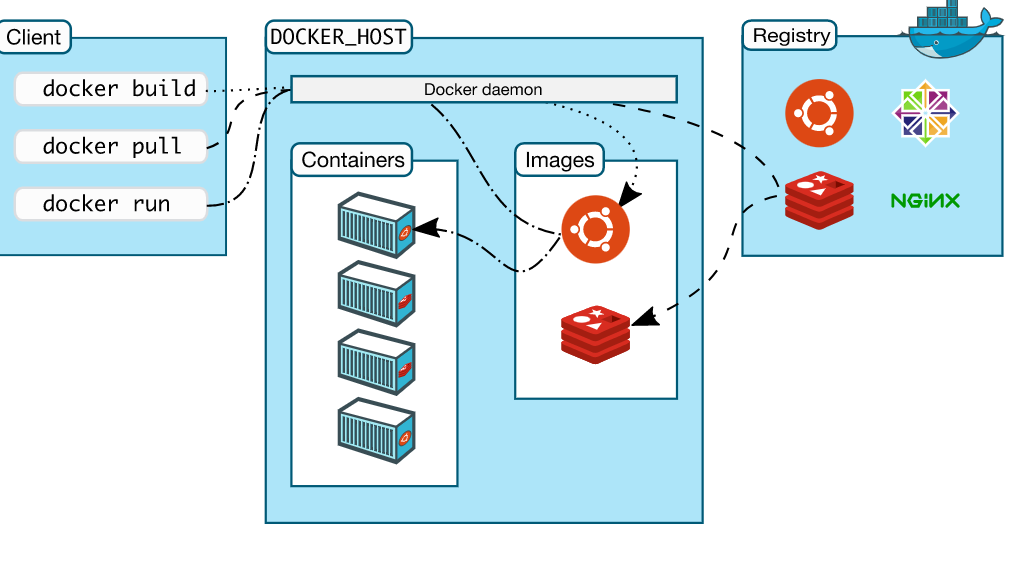
\includegraphics[width=0.8\textwidth]{SAC_B2_DockerStructure.png}
		\end{figure}
		
		\subsubsection{Concetti}
		Gli elementi che compongono Docker sono i seguenti:
		\begin{itemize}
			\item Container Management a cura di \verb*|Containerd|
			\item Container Engine a cura di \verb*|Docker|
			\item Data Management a cura dei file systems
			\item Orchestration a cura di \verb*|Docker-compose|, \verb*|Docker-swarm|, \verb*|Kubernetes|
		\end{itemize}
		
		\paragraph{Containerd}
		Si occupa dell'astrazione e della esecuzione dei container a basso livello. Le sue funzioni principali, esposte tramite API, sono:
		\begin{itemize}
			\item Esecuzione dei container (usando \verb|runc|)
			\item Gestione delle immagini dei container
			\item Push/Pull delle immagini nel registro dei container.
		\end{itemize}
		Containerd è a sua volta un'astrazione di \verb*|runc|. I molteplici strati su cui è costruito Docker sono fatti per semplificare la portabilità sia tra container runtimes (ad esempio Kubernetes usa runtime differenti) sia tra diversi sistemi operativi (grazie al fatto che containerd è stato portato per molteplici OS).\\
		
		Docker è un container engine usato per:
		\begin{itemize}
			\item Assemblare container
			\item Gestire container
			\item Eseguire applicazioni container-izzate
		\end{itemize}
		Fornisce quindi i benefici dei container per uno sviluppo DevOps friendly e scalabile.
		Ha un'architettura client-server:
		\begin{itemize}
			\item Un demone gestire i container (\verb*|dockerd|)
			\item Il client invoca i servizi del demone (\verb*|docker|) tramite REST API o UNIX socket
		\end{itemize}
		Docker fornisce un repository delle immagini dei container mediante il \textbf{registro}, utilizzato per archiviare e accedere alle immagini container.\\
		
		Docker gestisce oggetti che possono essere \textbf{immagini} o \textbf{container}.
		Le immagini sono template read-only, contengono istruzioni per creare un container e possono anche essere derivate da altre immagini.\\
		Esempio: Apache httpd server, è basato su un immagine Linux che aggiunge file per lanciare Apache httpd.\\
		
		I container sono istanze eseguibili di un immagine, supportano operazioni di creazione, start/stop, cancellazione.
		L'interazione è basata su comandi docker o comandi a riga. I container sono definiti da file di configurazione e da immagini.
		
		\subsubsection{Container file-system}
		I container lavorano con i cosiddetti \emph{layered filesystem}, molto simile al meccanismo dei file usati per memorizzare i dischi delle macchine virtuali: la differenza principale di questi ultimi è che questo genere di filesystem ragionano a livello
		di file, non di blocchi.\\
		
		I container invece sono oggetti di lettura e scrittura ma solo il livello \textbf{superiore} è scrivibile in quanto basato sull'approccio Copy-On-Write: i layers delle immagini sono condivisi finché non vengono modificati, nel senso che i layer vengono scaricati e riutilizzati per tutte le immagini che li usano. Quando un container modifica un layer condiviso, i file modificati, e solo quelli, vengono copiati nel layer read-write succitato.
		\begin{figure}[ht]
			\centering
			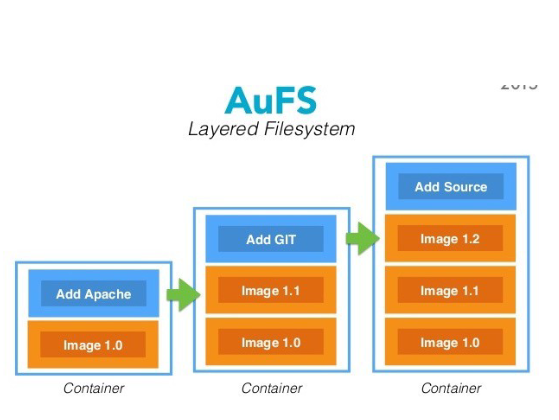
\includegraphics[width=0.5\linewidth]{images/SAC_B5_layeredfs}

			\label{fig:sacb5layeredfs}
		\end{figure}
		
		I container possono condividere la stessa immagine, con la differenza del livello superiore. Il sistema Copy-On-Write aumenta l'efficienza diminuendo il tempo di avvio e risparmiando spazio su disco.\\
		Sono disponibili anche altri approcci:
		\begin{itemize}
		    \item File system di unione: AUFS, sovrapposizioni
		    \item Istantanee: BTRFS, ZFS.
		    \item Dispositivi a blocchi Copy-On-Write.
		\end{itemize}
		\begin{figure}[ht]
		    \centering
		    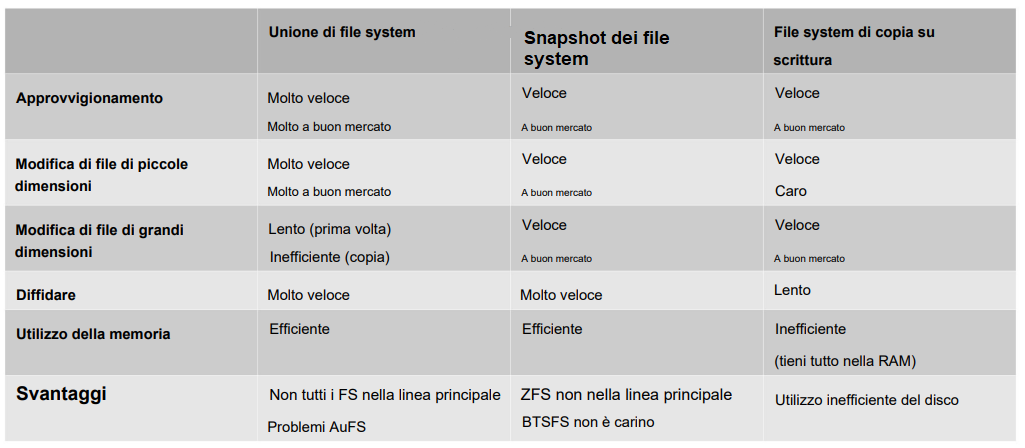
\includegraphics[width=0.8\textwidth]{SAC_B2_DockerFileSystem.png}
		\end{figure}
		
		Ogni livello del file system è una directory con un nome di una stringa esadecimale, la directory del livello più basso possiede:
		\begin{itemize}
		    \item File di collegamento
		    \item Directory diff con il contenuto del file system.
		\end{itemize}
		
		\subsection{Docker Swarm}
		Servizio di modello dichiarativo, descrive come deve essere fatto il deployment e come sono strutturati i vari containers.
		Attraverso un meccanismo di scaling automatico si definiscono i livelli di replicazione per ogni servizio.
		La riconciliazione dello stato desiderato serve per analizzare man mano lo stato corrente.\\
		
		\paragraph{Multi-host networking}
		Riusciamo a distribuire le nostre connessioni su più nodi attraverso un overlay network, un contenitore di interconnessioni mappato su un deployment distribuito, la configurazione della rete è automatica.\newline
		
		\paragraph{Service Discovery}
		DNS server integrato in swarm, per cui ogni container può comunicare con un altro container non su indirizzo IP ma attraverso un nome precedentemente definito.\newline
		
		\paragraph{Load Balancing}
		Attraverso il meccanismo interno di gestione della rete da parte di Docker riusciamo a gestire il carico in maniera bilanciato, andando a specificare come devono essere mappati i nostri nodi. Questo può servirci per capire come voler gestire l'Availability del nostro sistema, andando a istituire diverse policy.\newline
		
		\paragraph{Sicurezza}
		Docker Swarm è sicuro di default, la comunicazione criptata tra i vari nodi viene istituita tramite identificazione. E' possibile istituire certificati di autenticazione locali o esterni. \newline
		
		\paragraph{Aggiornamenti}
		Docker Swarm ci permette di poter fare degli aggiornamenti continui in maniera textbf{incrementale}, non c'è bisogno di aggiornare ogni cosa alla volta. Questo ci può permettere di evitare problemi di traffico su :
		\begin{itemize}
		    \item Hosts
		    \item Volumi
		    \item Immagini di registro
		\end{itemize}
		
		\subsubsection{Concetti di Docker Swarm}
		Uno swarm è una rete di nodi, dove all'interno vi è un hosts(fisico o virtuale), ognuno può essere:
		\begin{itemize}
		    \item Manager: Gestione dei membri e delle delegazioni. Riceve le descrizione per il deployment, può avere una distribuzione di unità di lavoro(task) su più nodi. Possono anche agire come Worker node ma questa policy di comportamento può essere modificata.
		    \item Worker: Manda in esecuzione i servizi swarm. Riceve ed esegue i task, gli agenti su questi nodi ricevono e monitorano i task
		    \item Entrambi.
		\end{itemize}
		Un nodo è un'istanza di sistema docker, tipicamente si ha un nodo per macchina, ma molti possono coesistere più macchine su un nodo.
		
		\subsection{Kubernetes}
		Auto-riparante, gestione del guasto dei container e rileva il container difettoso:
		\begin{itemize}
		    \item Container che non rispondono
		    \item Controlli definiti dall'utente
		\end{itemize}
		Operazioni non supportate:
		\begin{itemize}
		    \item Creazione automatica di container.
		    \item Nessun servizio integrato:
		    \begin{itemize}
		        \item Nessuna registrazione/controllo integrato.
		        \item Gli utenti possono scegliere.
		    \end{itemize}
		    \item Nessuna configurazione macchina/ Nessuna auto-installazione
		\end{itemize}
		
		\subsubsection{Componenti}
		\begin{itemize}
		    \item Nodi: Host che eseguono componenti containerizzati.
		    \item Pods: Componenti del carico di lavoro dell'applicazione.
		    \item Control Plane: API per la gestione dei container
		    \item Service: Espone un'applicazione in esecuzione su uno o piu Pod. Rende l'applicazione accessibile attraverso la rete
		\end{itemize}
		\begin{figure}[h]
		    \centering
		    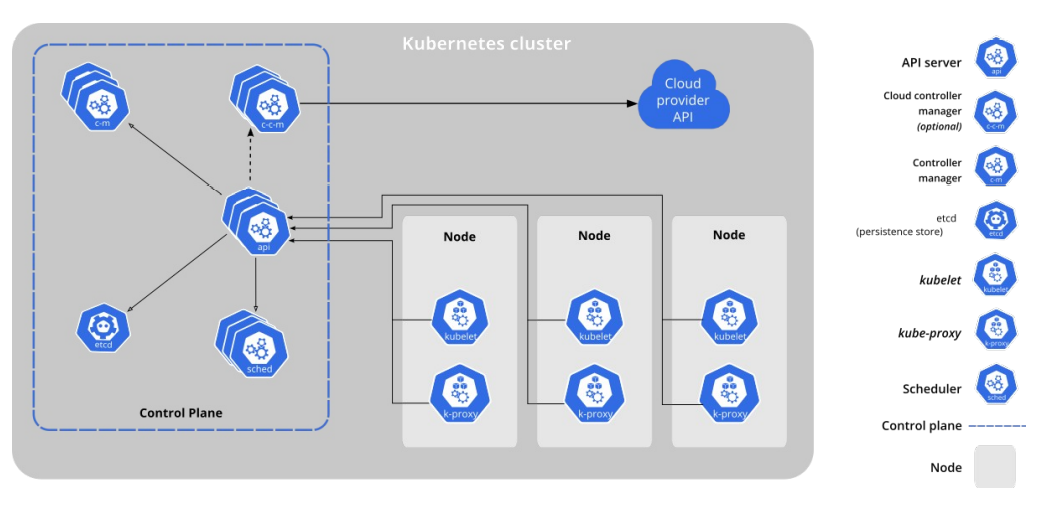
\includegraphics[width=0.8\textwidth]{SAC_B2_KubernetesComponents.png}
		\end{figure}
		
		\paragraph{Pod}
		Unita di carico di lavoro di base in Kubernetes, esistono più tipi di pod:
		\begin{itemize}
		    \item Pod contenitore singolo: caso più comune, viene eseguito un mapping 1 a 1 con i containers
		    \item Pod contenitori multipli: Un pod contiene più applicazioni complesse, stretto accoppiamento dei contenitori
		\end{itemize}
		Template Pod:
		\begin{verbatim}
		apiVersion: batch/v1
		kind: Job
		metadata:
		    name: hello
		spec:
		    template:
		        # This is the pod template
		        spec:
		            containers:
		            - name: hello
		                image: busybox
		                command: ['sh', '-c', 'echo "Hello, Kube!" && sleep 3600']
		            restartPolicy: OnFailure
		# The pod template ends here}
		\end{verbatim}
		
		Se viene modificato un modello pod, i pods vengono ricreati da un nuovo modello. Il modello Pod puo specificare i volumi, simile ai volumi Docker. Ogni pod ha un IP e i vari contenitori all'interno dello stesso pod possono comunicare utilizzando interfaccia di loopback.
		
		\paragraph{Control plane}
		La gestione delle applicazioni viene fatta attraverso chiamate API, le configurazioni vengono salvate tramite una struttura chiave valore.
		
		\paragraph{Scheduler}
		Tiene traccia dei pods, si concentra sui nuovi pod che non vengono assegnati a dei nodi, mentre gestisce l'assegnazione dei task ai vari nodi. Implementa funzioni per il bin-packing, bilanciamenti e gestioni delle ridondanze.\\
		
		\paragraph{Controller Manager}
		Gestisce i processi del controller, la sua implementazione di riferimento è quella del kube-controller-manager, è un controller specifico per il cloud che ha accesso alle API del provider. Vi sono poi altri controller, per vari aspetti dell'architettura:
		\begin{itemize}
		    \item Nodi.
		    \item Replicazione.
		    \item Endpoints.
		    \item Service account e token.
		    \item Instradamento.
		    \item Servizi: bilanciamento del carico del cloud.
		\end{itemize}
		
		\newpage
		\section{Serverless}
		La filosofia serverless vede come componente principale, la possibilità di astrarre completamente la gestione e la manutenzione dei server, delegandola al provider, permettendo a chi sviluppa di dedicarsi completamente allo sviluppo software. Il provisioning e il deployment di tutto lo stack necessario per eseguire l’applicazione è completamente managed: chi sviluppa dovrà preoccuparsi di fornire una definizione
		del software che sta scrivendo, che può essere un’immagine di un container o, a volte, anche meno.
		Se facciamo un confronto con le architetture IaaS dove si ha un controllo completo sull'infrastruttura, l'approccio senza server è un ridimensionamento automatizzato monitorato dal provider. Si ha un arresto del servizio quando non viene utilizzato, e l'utente deve preoccuparsi solo dell'aggiornamento del proprio software.
		\begin{table}[ht]
			\centering
			\begin{tabular}{|l|l|l|}
			\hline
			            & Serverless               & IaaS                    \\ \hline
			Scalabilità & Automatizzata            & Gestita dall'utente     \\ \hline
			Monitoring  & Gestito dal provider     & Gestito dall'utente     \\ \hline
			Costi       & Sulla capacità consumata & Sulla capacità allocata \\ \hline
			Sicurezza   & Gestita dal provider     & A carico dell'utente    \\ \hline
			\end{tabular}
		\end{table}
		I principali vantaggi sono:
		\begin{itemize}
		    \item Gestione: Nessuna preoccupazione per la gestione e la governance dell'infrastruttura.
		    \item Costi: Test, risoluzione dei problemi, controllo degli accessi esternalizzati al fornitore di servizi cloud.
		    \item Scalabilità e disponibilità: Il ridimensionamento orizzontale è automatico ed elastico. La tolleranza ai guasti è un problema del fornitore di servizi cloud
		    \item Riduzione al minimo della latenza: Le funzioni serverless in genere non operano da un singolo server di origine in modo che l'utente possa reindirizzato al server più vicino
		    \item Riduzione della complessità del software: Le funzioni devono essere semplici per poter essere deployate serverless e ciò aiuta a risolvere i bug e rilasciare aggiornamenti
		    \item Miglioramento della produttività del software: separazione di sviluppatori software da amministratori dell'infrastruttura
		\end{itemize}
		Vi sono due categorie di servizi serverless:
		\begin{itemize}
		\item Backend as a Service $\rightarrow$ Google Firestore
		\item Function as a Service $\rightarrow$ Google Functions
		\end{itemize}
		
		\subsection{Backend as a Service}
		Tipicamente il backend fornisce un servizio ad altre applicazioni sotto forma di API messe a disposizione per gli sviluppatori. Alcuni esempi possono essere Cloud Databases, servizi di autenticazione e autorizzazione, notifiche push etc.
		
		\subsection{Function as a Service}
		Se il software può essere suddiviso in funzioni ancora più piccole dei microservizi che esse servono allora queste possono essere deployate su server esterni in modo da separare lo stato dei server, e quindi affrancandosi dal bisogno di gestire l'infrastruttura, dalle funzioni stesse. Così facendo abbiamo una logica a grana ancora più fine in cui varie funzioni compongono un microservizi e, a loro volta, diversi microservizi costituiscono l'applicazione monolitica.
		Le caratteristiche principali delle Functions sono:
		\begin{itemize}
		\item Stateless: Inerentemente parallele, sono facilmente scalabili
		\item Effimere: Quando non utilizzate vengono dismesse. Non c'è persistenza
		\item Event-driven: Determinate condizioni di attivazione scatenano un'azione che viene eseguita
		\item Completamente gestite dal cloud provider
		\item Modello di costi per uso: ad esempio la RAM viene misurata in quantità occupata al secondo
		\item Business logic: Ci si concentra solo sulle funzionalità e non sull'infrastruttura
		\end{itemize}
		Gli utilizzi principali sono in quegli scenari in cui lo scaling automatico può fare la differenza, dove cioè ci sono grosse differenze di traffico tra il picco e il minimo oppure dove ci sono prolungati periodi di idle e workload incerti e variabili.
		\\ Gli svantaggi sono legati a doppio filo ai vantaggi che porta questa tecnologia:
		\begin{itemize}
		\item Performance: I server hanno bisogno di un certo tempo per essere avviati, una volta che sono stati interrotti per mancato traffico. Questo può portare ad un aumento di latenza che risulta critico in determinati contesti (es. trading).
		\item Risorse limitate: Il provider potrebbe imporre dei limiti sulle risorse disponibili rappresentando un problema in scenario di High Processing Computing. Inoltre non tutte le funzioni sono compatibili con tutti i provider serverless.
		\item Minor controllo: L'infrastruttura è completamente gestita dal provider
		\item Monitoring e Debugging: Le metriche fornite dal provider potrebbero non essere sufficienti e il debug non praticabile
		\item Sicurezza: Problema della monocultura: Quando viene trovata una vulnerabilità nell'infrastruttura del provider, questa intacca tutti i clienti che ne fanno uso
		\item Vendor Lock-in: Non c'è standardizzazione tra i provider
		\end{itemize}
		
		\subsection{OpenWhisk}
		OpenWhisk promuove principalmente l’evitare il vendor lock-in, infatti è interamente open source (Apache license). Il modello di programmazione prevede la definizione di un trigger al quale è associata una regola che, qualora si verifichi, attiva un’azione.
		Ogni azione ha delle caratteristiche abbastanza comuni:
		\begin{itemize}
		    \item Le azioni devono essere idempotenti: $\mathbf{T(T(x)) = T(x)}$
		    \item Devono essere parallelizzabili
		    \item Possono essere eseguite più volte rispetto allo stesso evento. Quindi l'ordine di esecuzione non è lo stesso dell'ordine di invocazione
		    \item Ogni operazione non deve essere dipendente dall'azione(non vi è uno stato interno)
		    \item Le azioni non sono atomiche
		\end{itemize}
		Le azioni hanno un input e un output, hanno una struttura a dizionario (chiave-valore), in cui la chiave è una stringa e il valore è un JSON. Ogni azione è definita da:
		\begin{itemize}
		    \item Namespace
		    \item Package name
		    \item Action name
		\end{itemize}
		Le azioni possono operare con doppia semantica:
		\begin{itemize}
		    \item Richiesta/Risposta: Bloccante. Ritorna i dati solo quando l'azione è generata
		    \item Fire and Forget: L'azione una volta terminata genera un evento (una sorta di callback) per comunicarlo 
		\end{itemize}
		Quando lavoriamo in Fire and Forget è importante l'elemento dell'Activation Record: dove per ogni invocazione dell'azione viene memorizzato in un log:
		\begin{itemize}
		    \item Activation ID
		    \item Nome della funzione (con namespace)
		    \item Timestamps(Inizio e fine
		    \item Logs
		    \item Valore di risposta
		\end{itemize}
		WEB actions
		Azioni per generare applicazioni web. Possono operare ricevendo richieste HTTP, settando headers status code e gestire i cookies. Restituiscono un body HTML. La risposta è sempre un JSON object
		Gestione delle risorse
		Openwhisk supporta limiti per l'utilizzo delle risorse nelle funzioni. Possiamo imporre dei limiti relativi a:
		\begin{itemize}
		    \item Tempo di esecuzione
		    \item Utilizzo della memoria
		    \item Output size
		    \item Numero delle esecuzioni ricorrenti
		    \item Activation rate
		\end{itemize}
		I trigger sono un canale nominativo di una classe di eventi che operano su una sorgente dati. Le regole definiscono un vincolo tra i trigger e le azioni che verranno eseguite.
		\\Process model:
		\begin{itemize}
		    \item NGINX: Gestisce le richieste in arrivo
		    \item Kafka: coda di messaggi
		    \item DOcker: Vengono eseguite delle funzioni
		    \item CouchDB: Log e storage di metadati
		\end{itemize}
		
		\begin{figure}[ht]
		\centering
		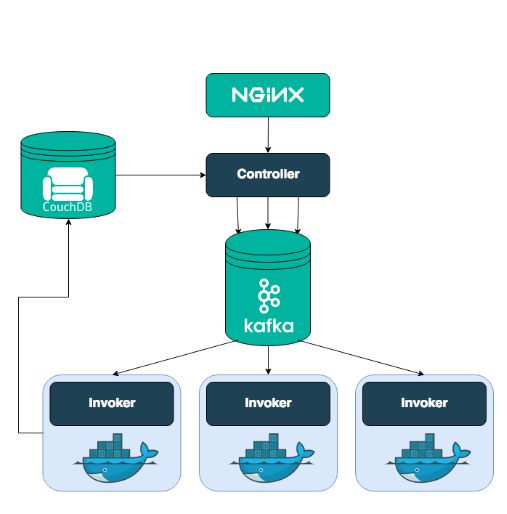
\includegraphics[width=0.5\linewidth]{SAC_B4_openwhisk}
		\label{fig:sacb4openwhisk}
		\end{figure}
		
		\subsection{OpenFaaS}
		Usato negli scenari di produzione.
		
		\subsection{AWS Lambda}
		Piattaforma per computing serverless. Fa parte dell'ecosistema Amazon, può interagire infatti con tutti i servizi AWS:
		\begin{itemize}
		    \item DynamDB
		    \item S3
		    \item AWS Step: un modo per andare a definire funzioni complesse, per esempio analizzando dei dati(Ingestion - Istanziamento delle macchine di un cluster spark - Esecuzione dell'app che esegue l'analisi - Alla fine spegnere il cluster ). Tutte queste operazioni di automazione di microfunzioni possono essere definite con il linguaggio AWS step. Sostanzialmente si istanzia un file JSON dove ogni passo corrisponde un'invocazione di una funzione lambda come effettuare un'azione o far partire un trigger. Strumento molto utile per l'automazione.
		\end{itemize}
		Prezzi
		\begin{itemize}
		    \item Richieste: Costo per un 1M
		    \item Costo per un 1GB di ram al secondo
		    \item Free Tire: 1M di rew, 400GBxsec per month)
		\end{itemize}
		Esempio:
		\begin{itemize}
		    \item Richiste: 3M di invocazioni: 0.2\$ x(3-1(franchigia)) = 0.4\$
		    \item Durata: 3M x 0.5GB x 1sec: 18.3\$
		\end{itemize}
		Layer:
		Il contesto di esecuzione può essere già noto o una runtime specifica.
		Gli eventi possono essere:
		\begin{itemize}
		    \item Custom: free format, inerenti per una determinata applicazione
		    \item Service Event: La struttura in questo casa è legata a qualcosa che sta succedendo nella piattaforma Amazon. in questo caso sarà schematizzata con determinati tipi di indici di un JSON.
		\end{itemize}
		Il runtime decide quanti containers mandare in esecuzione in base alle richieste, anche qui le funzioni sono regolate da trigger. Stesso approccio arriva nelle Google Functions( Supporta JS, Python, GO, Java).
		
		\subsection{Google Functions}
		Supportano molti tipi di eventi:
		\begin{itemize}
		    \item HTTP requests
		    \item Cloud Storage
		    \item Pub/Sub system
		    \item Cloud Firestore
		    \item Firebase
		\end{itemize}
		Triggers
		Possono essere invocati tramite righe di comando o console web.
		Ogni evento in questo caso ha la sua struttura dati.
		Il modello di costo è analogo ai sistemi precedenti quindi basato sempre sul tipo di runtime e al tempo di esecuzione. Per cui la qualità e l'efficienza del codice influisce molto sul costo dell'applicazione. 
		
		\newpage
		\section{Virtualized Storage}
		La virtualizzazione dello storage è necessaria per incrementare la capacità di memoria unendone molteplici dischi poiché non esiste nessun disco che possa soddisfare lr richieste di exabyte di dati dei datacenter. Così facendo anche il troughput aumenta dato che molte unità possono operare in parallelo e suddividersi il carico. Infine, la virtualizzazione dello storage aumenta la disponibilità dei dati e riduce i costi.
		Possiamo classificare i metodi di virtualizzazione secondo due caratteristiche:
		\begin{itemize}
		\item Granularità 
		\item Scope
		\end{itemize}
		
		\subsection{Granularità della virtualizzazione}
		Il tipo di granularità dipende dall’altezza alla quale avviene la virtualizzazione. Il mapping può essere fatto al di sotto del filesystem (virt. a blocchi), col quale viene offerto un dispositivo a blocchi virtuale che si occupa della loro gestione, oppure al di sopra di esso (virt. file based), dove viene semplicemente astratta la locazione fisica del file.
		
		\subsection{Block Based}
		Lo storage viene visto come un pool di blocchi logici su cui viene costruito il file system. Così facendo non è necessario che i dischi siano residenti sulla macchina ma possono essere distribuiti e remoti. Il file system spazierà quindi su diversi dischi in locazioni differenti. Occorre il supporto di quest'ultimo nella gestione di filesystems distribuiti.
		Tipicamente si lavora con strumenti come SCSI, un linguaggio comandi per i dischi, incapsulati tramite protocolli di rete.
		\begin{itemize}
		    \item TCP/IP
		    \item FCP (Protocolli in canali fibra)
		    \item InfiniBand, attraverso il remote DMA support
		\end{itemize}
		Un blocco viene identificato tramite la coppia 
		\begin{itemize}
		    \item LUN: Logic Unit Number.
		    \item LBA: Logical Block Address.
		\end{itemize}
		Il primo rappresenta il nome del dispotivo (es. \verb*|sda|) mentre il secondo indica dove si trova il blocco all’interno di tale LUN. LBA potrà essere, ad esempio, la terna che identifica i settori in un disco rotativo.\\
		
		Per astrarre anche il tipo di disco utilizzato, si utilizza un altro livello di indirezione, infatti, dagli LBA fisici, vengono ricavati degli LBA logici, che verranno utilizzati effettivamente nella comunicazione. Occorre però tenere traccia delle associazioni logico-fisiche, da qui l'introduzione dei \textbf{metadati}: tabelle che contengono le associazioni LBA fisico - LBA logico. Grazie ai metadati è possibile implementare agilmente la ridondanza mappando lo stesso blocco logico in più blocchi fisici.\\
		
		Un’altra utilità dei metadati è quella di realizzare il \emph{load balancing} dell’utilizzo dei dischi fisici: se ho un file contiguo, posso mappare i blocchi logici contigui su dischi fisici diversi. In questo modo, il blocco logico contiguo viene letto, sostanzialmente, in
		parallelo, perché presente su dispositivi fisici diversi.\\
		
		Ovviamente, questi metadati sono importantissimi, poiché rappresentano
		l’informazione (senza metadati, gli id fisici sono inutili, poiché il fs ragiona per indirizzi logici), pertanto vanno anch’essi ridondati.
		
		\subsection{Migliorare le prestazioni}
		Attraverso un sistema RAID possiamo avere delle performance maggiori, in quanto il throughput raddoppia, per cui il tempo di risposta si dimezza.\\
		 
		Mediante la tecnica LVM, Logical Volume Management, usata in sistemi linux per mappare eventi logici in estensioni fisiche (blocchi su dischi), si costruisce un file system con vari LE (Logical Extents) collegati a dei PE (Physical Extents) distributi su dischi diversi, per bilanciare meglio il carico. 
		I suoi concetti chiave sono:
		\begin{itemize}
		    \item PV: Volume fisico.
		    \item PE: Estensione fisica.
		    \item LV: Volume logico.
		    \item LE: Estensione logica.
		\end{itemize}
		E' possibile avere due approcci per accedere ai metadati:
		\begin{itemize}
		    \item Accesso trasparente: La richiesta viene fatta per il Logical Extent e sarà compito del Softare Defined Storage tradurla in PE
		    \item Accesso ai metadati tramite API: I file system interrogano i metadati per un dato LE e sarà compito loro effettuare la traduzione.
		\end{itemize}
		Se il primo approccio è meno oneroso per i file system del secondo, è penalizzato in quanto a scalabilità.\\
		
		Alcune features facilmente implementabili nell'approccio block-based:
		\begin{itemize}
		    \item Snapshotting: Attraverso il sistema a blocchi è facile implementare gli snapshot: tutti i blocchi di un file vengono marchiati come copy-on-write e le scritture successive produrranno una copia del file. Questa operazione avviene solo sui metadati non sui blocchi effettivi del disco.
		    \item De-duplicazione dei dati: Evitare copie dello stesso blocco, meccanismo intrinseco dello snapshotting, che possono far risparmiare ingenti quantità di memoria.
		\end{itemize}
		
		\subsection{Filesystem-based}
		Utilizza i file come unità base di memorizzazione e sfrutta file system di rete:
		\begin{itemize}
		    \item NFS
		    \item SMB/CIFS
		\end{itemize}
		L'accesso alle directory e ai file avviene tramite delle API di rete che mascherano le syscalls come se avvenissero in locale. La ridondanza viene gestita internamente e non presenta la necessità di metadati per mappare LE a PE.
		
		\subsubsection{NFS}
		E' un sistema molto veloce basato su RPC (Remote Procedure Call). Ha visto diverse release e numerose funzionalità sono state aggiunte negli anni.
		
		\subsubsection{SMB/CIFS}
		Un filesystem completamente diverso, che permette di accedere a delle risorse, con relativi protocolli, di vario genere (Stampanti, Porte, Files).
		
		\subsection{Obiettivi virtualizzazione dello storage}
		Con obiettivo della virtualizzazione si intende la dimensione e la visiblità dello storage che vogliamo avere. Si declina in tre principali infrastrutture:
		\begin{itemize}
		    \item DAS: Identifica un disco collegato localmente ad una macchina.
		    \item NAS: Identifica un disco visibile a più macchine.
		    \item SAN: Identifica più dispositivi dedicati allo storage.
		\end{itemize}
		\subsubsection{DAS}
		Si tratta di un disco esterno collegato a un host. Le interazioni si basano su protocolli non di rete (ad esempio il disco può essere collegato mediante una periferica USB).
		Quando il disco viene collegato all'host, viene preso in carico dal sistema operativo attraverso i driver. I volumi logici sono tipicamente visibili localmente ma possono essere esposti anche sulla rete. 
		\subsubsection{NAS}
		Non vi è bisogno di collegare direttamente il server che deve fruire dello storage allo storage stesso. Il server che necessita di accedere allo storage non deve essere collegato direttamente a quest'ultimo ma la comunicazione avviene mediante lo stack TCP/IP. Il controller del disco non è più il server che deve fruire dello storage, ma sarà il sistema operativo presente sul NAS stesso, che esporrà delle interfacce per accedervi. L’accesso remoto può essere fatto sia in modo block-based che in modo filesystem-based.
		I componenti principali sono:
		\begin{itemize}
		    \item Memorizzazione: viene effettuato attraverso dischi, SSD o HDD.
		    E' possibile scegliere quale tipo di disco utilizzare anche in base alla metrica UBER.\\
		    UBER è una metrica per il tasso di occorrenza di errori di dati, pari al numero di errori di dati per bit letti durante l'intera vita di un SSD. Matematicamente:
		    \begin{center}
		     $ UBER= \frac{number of data errors}{number of bits read}$
		    \end{center}
		    \item Controller: RAID per gestire i dischi collegati in serie. I controller RAID possono essere sia software che hardware. Nel primo caso tipicamente si usano degli standard open e i dischi sopravvivono alla rottura del controller mentre nel primo caso la rottura porterebbe alla perdita dei dati sui dischi.
		    \item Interfacce di rete: costituite da varie schede di rete ad alta velocità capaci di supportare anche connesione a 10Gbps.
		\end{itemize}
		\subsubsection{SAN}
		Questo tipo di reti possono avere dati di archiviazione fino all'ordine di Exabyte. Vi possono essere più livelli:
		\begin{itemize}
		    \item Host Layer: Il frontend che accede ai dati, che generalmente viene replicato (i.e. una rest api che accede ai dati) e che rappresenta l’endpoint per accedere alla SAN
		    \item Fabric Layer: La fibra ottica che mette in collegamento gli switch e i router
		    \item Storage Layer: Dischi di archiviazione pensati per esporre i dati in maniera block-based e in modo estremamente flessibile e reliable RAID e JBOD. L’accesso è tipicamente derivante da protocolli simil-SCSI.
		\end{itemize}
		\subsection{Software defined storage}
		La vera sfida di questa tipologia di archiviazione è la \text{disponibilità} e l'affidabilità dei dati, i quali devono essere sempre disponibili e non possono essere persi o danneggiati.\\
		Inoltre devono essere anche gestibili e scalabili, quindi devono essere recuperati in modo in efficiente e condivisi tra loro, ma a causa della loro dimensione il sistema deve anche essere capace di gestire il gran numero di richieste.
		All’interno dello storage pool avrò dischi diversi di vendor differenti con molteplici filesystem, motivo per il quale serve un layer che astragga la complessità e mi permetta di gestire SAN estremamente eterogenee. Concetto di hardware independence\\
		Le funzionalità chiave per fornire gli attributi richiesti da questo tipo di archiviazione sono:
		\begin{itemize}
		    \item Automazione: cioè la gestione semplificata che riduce i costi di manutenzione dell'infrastruttura di storage.
		    \item Interfacce standard: tramite API per gestione, provisioning e manutenzione di dispositivi e servizi di archiviazione.
		    \item Modalità di accesso: Interfacce Block, File e Object.
		    \item Scalabilità.
		\end{itemize}
		Alcuni esempi sono:
		\subsubsection{Ceph}
		Ceph è un filesystem che abilita SDS in maniera estremamente semplice. Permette di distribuire i dati su più dischi mediante l’algoritmo
		CRUSH (hash-based load balancing). Da un punto di vista architetturale, Ceph riutilizza il concetto di metadati (come in block-based) e introduce il concetto di journaling, quindi tutte le operazioni sul filesystem (distribuito) sono atomiche.
		Due concetti fondamentali:
		\begin{itemize}
		\item Meta Data Server distribuito con supporto al bilanciamento del carico per le operazioni di apertura file, creazione e lista directory
		\item Reliable Autonomic Distributed Object Store che gestisce il filesystem block based per le operazioni effettive di scrittura e lettura
		\end{itemize}
		
		\newpage
		\section{Software Defined Networks}
		\subsection{NFV: Network Function Virtualization}
		Il termine Network Functions Virtualization (NFV) nell'ambito delle reti di telecomunicazioni indica un approccio architetturale che sfrutta le tecnologie IT per virtualizzare intere classi di funzioni dei nodi di rete come blocchi elementari che possono essere interconnessi per implementare servizi di comunicazione.
		Una funzione di rete virtualizzata consiste in una o più macchine virtuali che gestiscono diversi software e processi su server standard ad alta capacità, switch e dispositivi di memoria o anche su un'infrastruttura in cloud, invece di utilizzare differenti dispositivi hardware per ogni funzione di rete.
		In questo modo, elaborazioni tradizionalmente residenti nei nodi di rete possono essere eseguite in modo centralizzato sulla macchina virtuale, alleggerendo il carico elaborativo sui nodi di rete che assumono, rispetto alla funzione virtualizzata, il ruolo di attuatori.\\
		L'approccio è mirato sia a ridurre il costo dei nodi di rete (per la minore complessità richiesta o in casi estremi eliminando la necessità del nodo fisico stesso) che a integrarsi in una gestione di rete di tipo SDN, contesto in cui le NFV possono essere usate in modo sinergico.
		\\L'obiettivo principale è quello di instradamento, definizione policy di routing complesse che si possano adattare bene a scenari di virtualizzazione, ricordiamo infatti che la VM può comunicare utilizzando apparati fisici o bridge virtuali, o anche switch e router.
		\newpage
		\subsection{SDN: Software defined network}
		\subsubsection{Motivazioni}
		Attraverso la definizione di reti dal software, si cerca di soddisfare alcuni requisiti fondamentali:
		\begin{itemize}
		    \item Condivisione delle risorse.
		    \item Isolamento delle prestazioni: i flussi di traffico non devono interferire, le soluzioni possono essere uno switch capace di gestire delle VLAN. E' necessario anche poter gestire un carico di lavoro variabile che può essere altamente variabile. 
		    \item Supporto alla ridondanza: La ridondanza è necessaria per la tolleranza ai guasti per cui è importante implementare alcuni algoritmi di gestione come alberi di copertura con un solo percorso disponibile che evita dei loop. 
		    Questo obiettivo da soddisfare può andare in conflitto con altri, come l'isolamento delle prestazioni o la condivisione delle risorse.
		    \item Riduzione dei costi OPEX e CAPEX tramite dispositivi hardware off-the-shelf e non più dedicati, quindi costosi.
		\end{itemize}
		L'obiettivo critico è quello di adattarsi a scenari che possono cambiare in maniera molto dinamica e che in caso di problemi repentini il sistema cloud deve essere capace di gestirli automaticamente.\\
		Alcune aree critiche rimangono:
		\begin{itemize}
		    \item Interazione controller: pacchetti inviati con grande latenza.
		    \item Problemi di prestazioni del piano dati: tabelle grandi e predicati complessi.
		    \item Scalabilità del controller: può diventare un colo di bottiglia e l'utilizzo di più controller necessità l'implementazione di una coordinazione.
		    \item Ridondanza del controller.
		\end{itemize}
		Per capire meglio come funzionano le SDN occorre definire due elementi principali:
		\begin{itemize}
		\item Data Plane: Dove avviene la manipolazione dei pacchetti. Nel caso di un router è la parte che si occupa del forwarding dei pacchetti
		\item Control Plane: Dove vengono prese le decisioni per la gestione dei pacchetti. Nel caso di un router è la parte che si occupa dell'instradamento dei pacchetti
		\end{itemize}
		Il Software Defined Networking (SDN) è un’architettura per la realizzazione di reti di telecomunicazioni nella quale il piano di controllo della rete e quello di trasporto dei dati sono separati logicamente.\\
		Questa separazione logica permette da un lato la possibilità di gestire via software tutta la rete da un unico controller, garantendo così una maggiore scalabilità e standard di affidabilità e sicurezza della rete più elevati, dall’altro quella di utilizzare indifferentemente apparati prodotti dalle diverse aziende che non conteranno più al loro interno le funzioni di gestione favorendo, così, la nascita di una rete dinamica e non più legata al larghissimo numero di protocolli differenti attualmente utilizzati.\\
		SDN fornisce alla NFV i vantaggi di una connessione programmabile tra le funzioni di rete virtualizzate; la NFV, invece, mette a disposizione dell’SDN la possibilità di implementare le funzioni di rete tramite software su server COTS (Commercial off-the-shelf). Si ha, così, la possibilità di virtualizzare il controller SDN implementandolo su di un cloud che può essere facilmente migrato in qualsiasi posizione in base alle esigenze della rete.
		\subsubsection{Switch SDN}
		Uno switch SDN è un programma software o un dispositivo hardware che inoltra i pacchetti in un ambiente SDN. Deve supportare i protocolli SDN. Il primo e il più noto protocollo SDN è OpenFlow. Pertanto, uno switch SDN viene spesso chiamato anche switch OpenFlow. Esistono anche altri protocolli SDN sviluppati dai fornitori di switch SDN, come OpFlex, NETCONF, BGP (Border Gateway Protocol), XMPP (Extensible Messaging and Presence Protocol), ecc.\\
		Funzionamento\\
		Il piano di controllo (routing di alto livello) è disaccoppiato dall'hardware dello switch SDN, ma è implementato nel controller SDN (un'applicazione in esecuzione sul server o da qualche parte), che si trova tra i dispositivi di rete e le applicazioni.
		Ogni switch SDN nel modello SDN è programmabile dal controller SDN attraverso i protocolli SDN. Le comunicazioni tra applicazioni e dispositivi avvengono attraverso il controller SDN.\\
		Uno switch SDN è composto da porte e tabelle. I pacchetti arrivano e lasciano lo switch attraverso le porte. Le tabelle sono costituite da righe contenenti un classificatore e un insieme di azioni. Quando uno switch SDN riceve un pacchetto che non ha una riga corrispondente nella tabella, comunica con il controller SDN e chiede cosa fare con questo pacchetto. Il controller può scaricare un flusso sullo switch, che include il primo classificatore che meglio corrisponde al pacchetto e le azioni.
		Le azioni gestiscono il trattamento del pacchetto, che può essere l'inoltro alle porte, l'incapsulamento e l'inoltro al controllore, l'eliminazione del pacchetto o l'invio alla normale pipeline di elaborazione. Una volta che i predicati sono stati scaricati nella tabella degli switch, questi vengono processati in autonomia. Il predicato del matching può usare molti campi per stabilire la regola: può agire su campi che vanno dal livello più basso dello stack TCP/IP fino ai protocolli di trasporto. Uno switch SDN può, quindi, gestire qualsiasi livello dello stack, rendendolo molto efficace.\\
		Southbound API \\
		I messaggi che possono essere inviati tramite la southbound API sono:
		\begin{itemize}
		\item Controller to switch: Messaggi di controllo e configurazione
		\item Messaggi asincroni da switch a controller: Messaggi inviati quando è necessario l'intervento del control plane
		\item Messaggi simmetrici: Messaggi usati per controllo della salute dei dispositivi
		\end{itemize}
		Vantaggi SDN\\
		Un vantaggio generale dell'uso degli switch SDN è la facilità di controllo e configurazione del flusso. Con gli switch SDN, non è necessario recarsi presso le postazioni dello switch e accedere alla riga di comando per configurarlo. 
		È possibile controllare e programmare in remoto più switch attraverso un unico controller SDN che utilizza il protocollo SDN e fornisce API per gli switch SDN. 
		Altri vantaggi sono che sarà più facile effettuare il bilanciamento del carico anche a velocità di dati elevate e il traffico potrà essere isolato senza bisogno di VLAN, poiché il controller SDN funziona per rifiutare determinate connessioni.
		
		\newpage
		\section{Software Defined Data Center}
		L'applicazione dei principi di virtualizzazione ai data center nasce dall'esigenza di avere un sistema elastico e flessibile.
		\subsection{Punti di Vista}
		Ci sono diversi aspetti che un cloud provider deve tenere in considerazione, ciascuno di questi appartenente a punti di vista differenti:
		\paragraph{Utente}
		Un utente deve avere la percezione di avere una macchina per se. La scalabilità del sistema messa a disposizione dell'utente deve essere istantanea: in pochi istanti deve essere possibile per l'utente avere a disposizione altre macchine. Il sistema deve garantire una certa sicurezza: sui data center possono essere messi dati sensibili, pagando si deve essere certi che un team di persone competenti (con privilegi diversi) mantengano la piattaforma sicura. Il servizio offerto deve essere affidabile: le risorse sempre disponibili (ridondanza dei dati) e il downtime di pochi minuti all'anno.\\
		\paragraph{Ingegneristico}
		L'infrastruttura deve essere gestita sotto gli aspetti software e hardware, in particolare in termini di consumo energetico, raffreddamento e sicurezza (persone che hanno accesso ai sistemi).
		\begin{itemize}
		    \item Software: È necessario un sistema di monitoraggio per conoscere le macchine accese e le risorse utilizzate, in modo da sapere quanto far pagare i servizi.
		    \item Harware: I nodi di calcolo (host) vengono raggruppati in racks che possono essere raggruppati in
		    pods, dei container di racks (generalmente spostati usando dei camion) che presentano tre cavi: 
		    per la rete, energia e per il raffreddamento. I pods possono essere visti anche come dei mini data center, e rappresentano un'alternativa alla struttura gerarchica classica del data center tradizionale.
		\end{itemize}
		\subsubsection{Data Center Cloud}\label{data-center-cloud}
		Oggigiorno molti data center stanno migrando verso la struttura cloud. Ci si aspetta che un data center cloud rispetti determinati criteri e
		caratteristiche:
		\begin{itemize}
		\tightlist
		\item Conveniente
		\item Scalabile
		\item Realizzabile
		\item Sicuro
		\item Elastico
		\item Internet-based
		\end{itemize}
		\subsection{Infrastruttura}
		Il data center viene organizzato in blade systems, composti da un certo numero (solitamente 4) di blade (l'unità di computazione vera e propria) inserite all'interno di un chassis. Se nella blade troviamo componenti come RAM, CPU e hardware di rete, nello chassis si trova l'alimentazione, il sistema di raffreddamento e quello di monitoraggio. I blade systems vengono organizzati in racks, delle sorte di armadi che presentano degli switch utilizzati per l'interconnessione di più blade systems tra loro e il resto del datacenter. Nei racks sono presenti due tipi di switch:
		\begin{itemize}
		\tightlist
		\item top-of-rack: per la connessione di più elementi nello stesso rack
		\item end-of-row: per la connessione di racks sulla stessa fila
		\end{itemize}
		Le blades montano sistemi di storage di piccole
		dimensioni NVRAM o SSD (generalmente intorno ai 500Gb,
		1Tb) utilizzati per il caching dei dati e per far girare
		l'hypervisor, mentre l'unità di storage vera e propria
		dei data center consiste in una Storage Area Network
		(SAN), uno storage persistente che
		mantiene le copie delle immagini delle VM.
		
		\hypertarget{data-center-network}{%
		\subsubsection{Data Center Network}\label{data-center-network}}
		
		\hypertarget{struttura}{%
		\paragraph{Struttura}\label{struttura}}\mbox{}\\
		La rete di un datacenter presenta una topologia ad albero nel
		quale è possibile individuare diversi livelli (dal basso all'alto):
		
		\begin{itemize}
		\tightlist
		\item
		  Servers: si tratta dei blade systems,
		  rappresentano le foglie dell'albero e sono interconnessi tra
		  loro mediante dei collegamenti da 1-10Gbps.
		\item
		  Edge Layer: anche chiamato Access Layer, è
		  composto da switch top-of-rack ed eventualmente da
		  quelli di tipo end-of-row. In questo layer i
		  blade systems vengono connessi e vengono implementate
		  le funzioni di isolamento del traffico e di \emph{gestione dei
		  guasti}.
		\item
		  Aggregation Layer: su questo livello vengono
		  interconnesse zone separate dei datacenter
		  (interconnessione di pods). Il layer implementa
		  funzionalità di QoS per i flussi dati (è possibile
		  anche rallentarne alcuni in casi di sovraccarico). Traffic shaping in
		  caso di overload.
		\item
		  Core Layer: in questo layer si lavora
		  esclusivamente a livello di rete. Gestisce tutte le
		  connessioni con l'esterno e
		  l'instradamento in caso di failures (quando alcuni
		  link non sono disponibili), inoltre interagisce con la
		  SAN. Il livello di disponibilità delle risorse è estremamente
		  importante, serve infatti un'ottima politica di gestione in caso di
		  disponibilità critica.
		\end{itemize}
		
		\paragraph{Limiti della Topologia ad
		Albero}\label{limiti-della-topologia-ad-albero}\mbox{}\\
		Il principale problema di questa topologia sta nei \textbf{layer
		superiori} (aggregation e core), che possono diventare dei
		colli di bottiglia o essere soggetti a
		failures. La soluzione consiste nell'utilizzo
		della replicazione e nella \textbf{\emph{riprogettazione della
		topologia}}. Con una nuova topologia di tipo Fat Tree
		vengono messi a disposizione \textbf{\emph{più link nella parte
		superiore della rete}}, ottenendo una banda maggiore, e
		quindi maggiore scalabilità e \textbf{\emph{tolleranza
		ai guasti}}. La configurazione di rete utilizzata per ottenere
		questi risultati si chiama CLOS Network.\\
		\begin{figure}[ht]
			\centering
			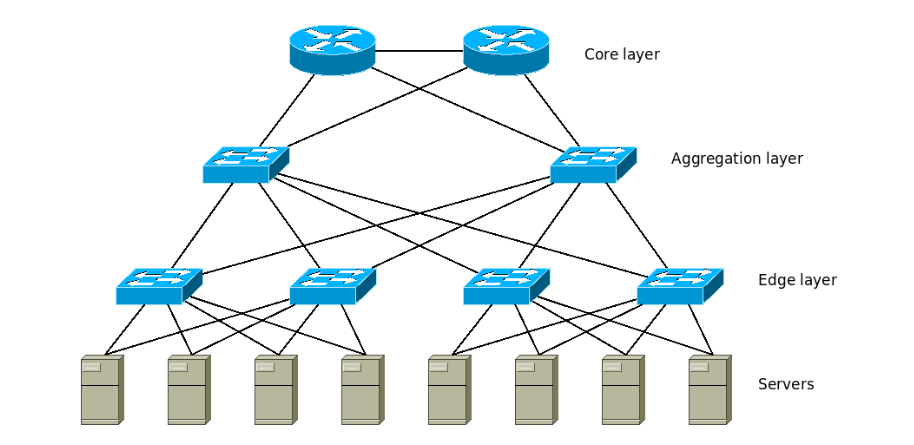
\includegraphics[width=0.7\linewidth]{SAC_B7_clos}
			\label{fig:sacb7clos}
		\end{figure}
		
		\paragraph{CLOS Network}
		Si considera il datacenter come
		un grafo, dove i nodi sono i server/switch e gli
		archi tra i nodi le connessioni. L'obiettivo di una rete di
		questo tipo è quello di minimizzare il numero di percorsi
		bloccati (in uso), minimizzando il numero di
		connessioni. Prima dell'introduzione della rete Clos, il numero di punti di incrocio doveva essere uguale al numero di ingressi moltiplicato per il numero di uscite. Questo approccio, noto come n-squared o n2, poteva portare rapidamente a un numero enorme di punti percorsi, con conseguenti costi significativi. nelle reti Clos gli switch sono stati organizzati in un'architettura a tre stadi che comprendeva uno stadio intermedio inserito tra gli stadi di ingresso (input) e di uscita (output). In questo modo, ogni switch di ingresso si collega a ogni switch intermedio che, a sua volta, si collega a ogni switch di uscita. Il risultato è una topologia non bloccante che richiede meno punti di incrocio rispetto alle reti di switch più convenzionali dell'epoca. Grazie alle reti Clos è possibile ri organizzare la rete per trovare un percorso che prima sembrava inaccessibile o bloccato. 
		
		\begin{quote}
		Google Data Center - Scenario La crescita del traffico per i
		data center Google segue la legge di Moore, raddoppiando ogni
		12/15 mesi. Questo aumento ha come conseguenza un \emph{aumento del
		numero di elementi di rete da interconnettere}. Nel 2004 il rapporto tra
		la banda gestibile dal dispositivo e quella entrante era di 10:1.
		È in scenari simili che l'adozione di una CLOS Network fa la
		differenza.
		\end{quote}
		
		\subsubsection{Scalabilità}\label{scalabilituxe0}
		
		La scalabilità rappresenta il problema principale
		di un datacenter. Quando si parla di scalabilità questa può essere
		verticale, si scala facendo un upgrade degli
		apparati hardware/software oppure orizzontale,
		basato sulla replicazione. Tra i due la \emph{scelta
		migliore}, nonché la più economica è quella della
		replicazione orizzontale, che consiste anche nel
		fare affidamento sulla generazione precedente, con un
		10\% in meno di performance su \emph{dispositivi che costano la
		metà}. Scelto il tipo di scalabilità rimane da decidere \emph{come
		replicare}. Anche per la replicazione sono disponibili
		due metodi:
		
		\begin{itemize}
		\tightlist
		\item
		  Replicazione \textbf{verticale}: dove un servizio complesso
		  viene suddiviso in sottoservizi ciascuno messo su un
		  dispositivo diverso
		\item
		  Replicazione \textbf{orizzontale}: che consiste nella
		  replicazione di oggetti identici
		\end{itemize}
		
		\paragraph{Architettura di un Web
		Cluster}\label{architettura-di-un-web-cluster}\mbox{}\\
		In generale, l'architettura tipica di un Web Cluster fa
		uso di entrambi i metodi di replicazione e si divide su due livelli:
		\begin{itemize}
		\item
		  Front-end: costituito dal web switch \emph{visibile
		  all'esterno come un unico indirizzo IP pubblico}, detto \textbf{Virtual IP}. Il ruolo
		  dell web switch nell'architettura è quello di direttore
		  d'orchestra. Può essere implementato a tutti i livelli (hardware,
		  kernel-level, applicativo). Deve avere delle
		  funzionalità per il bilanciamento del traffico, e per
		  questo si hanno due opzioni:
		
		  \begin{itemize}
		  \tightlist
		  \item
		    Switch di Livello 4 (Trasporto): vengono utilizzate
		    delle binding tables (strutture dati) per
		    tenere traccia delle connessioni TCP. Il
		    3-way-handshake viene mediato dallo switch e poi
		    portato avanti dal backend server a cui è diretto il pacchetto.
		  \item
		    Switch di Livello 7 (Applicativo): si tratta di
		    nodi più intelligenti che lavorano in termini
		    richiesta, e possono tenere traccia delle sessioni
		    utente. Il 3-way-handshake viene gestito
		    interamente dallo switch, che deve conoscere la richiesta
		    per sapere dove inoltrarla.
		  \end{itemize}
		
		  Non c'è una soluzione migliore dei due. Possono essere adottate
		  entrambe in base al contenuto del traffico.
		
		  \begin{quote}
		  Esempio: Instagram La \emph{maggior parte del
		  contenuto del contenuto} è un contenuto statico
		  (immagini), pertanto si possono usare switch di livello 4. Per
		  tutte quelle funzionalità che utilizzano delle API per
		  consigliare post, chi seguire, è possibile utilizzare
		  switch di livello 7.
		  \end{quote}
		\item
		  Backend: insieme di server \emph{configurati con IP
		  privati} che utilizzano il front-end per le comunicazioni con
		  l'esterno
		\end{itemize}
		
		\hypertarget{limiti}{%
		\paragraph{Limiti}\label{limiti}}\mbox{}\\
		I limiti della scalabilità sono strettamente collegati alla
		consistenza dei dati: le repliche devono essere
		mantenute aggiornate. I colli di bottiglia
		possono verificarsi sia negli switch che nella
		rete dei datacenter. Inoltre, è opportuno considerare la
		crescita dei datacenter anche in relazione al
		consumo energetico che richiedono.
		
		\hypertarget{traffico}{%
		\subsubsection{Traffico}\label{traffico}}
		
		Quando si parla di traffico di un datacenter si deve far riferimento a
		piccoli gruppi di cluster interconnessi. Si possono identificare dei pattern nella comunicazione tra i nodi di un cluster. Infatti, i nodi di un rack tipicamente comunicano con i nodi dello stesso rack, motivo per il quale vanno messi vicini:
		non necessariamente sulla stessa macchina fisica, poiché
		potrebbero entrare in competizione per le risorse causando un
		overload e di conseguenza un calo di prestazioni, ma
		neanche lontani per \emph{evitare di spostare grandi
		quantità di traffico}. Vi è anche un altro pattern riconoscibile: alcuni nodi sono particolarmente propensi a ricevere da tutti gli altri nodi (e collateralmente ad inviare). Questi nodi devono essere messi in una posizione \textbf{baricentrica} all'interno del datacenter. Inoltre, è opportuno spostare tutte quelle
		operazioni che occupano traffico come i backup durante le
		ore notturne, quando il server è meno probabile che debba
		soddisfare le richieste degli utenti.
		
		\subsubsection{Gestione del Data Center}\label{gestione-del-data-center}
		
		Il posizionamento e la migrazione delle macchine
		virtuali può essere utilizzata come soluzione a diversi problemi:
		
		\begin{itemize}
		\tightlist
		\item
		  Bilanciamento del carico
		\item
		  Consumo energetico: Consolidare server idle può aiutare a risparmiare energia
		\item
		  Utilizzo della rete: Le VM possono cambiare i loro pattern di carico di lavoro, analizzando i dataset differenti e le differenti interazioni tra i pattern. Non è necessario re-deploiare la VM se si preserva la località della rete.
		\item
		  Gestione del calore: Bisogna evitare i cosiddetti \textbf{hotspot}, ovvero le concentrazioni di server ad alta utilizzazione e cioè ad alta produzione di calore. Le macchine negli hotspot lavoreranno a maggiore temperatura e quindi avranno una maggiore usura. Inoltre se alcune macchine non vengono utilizzate è possibile spegnere l'impianto di condizionamento per tale area di modo da risparmiare notevole energia.
		\end{itemize}
		
		\hypertarget{reti-esterne}{%
		\paragraph{Reti Esterne}\label{reti-esterne}}\mbox{}\\
		Vi sono altri problematiche che vanno oltre quelle del datacenter e 
		riguardano l’instradamento di traffico fra più datacenter per
		applicazioni distribuite.
		I possibili punti di congestione sono:
		\begin{itemize}
			\item \textit{last mile}: Dall'uscita della rete al client finale
			\item \textit{first mile}: Dal datacenter all'ingresso della rete
			\item \textit{peering point}: Punti di scambio fra AS
		\end{itemize}
		La congestione non è sempre un problema \emph{vicino al
		datacenter}. Spesso può essere causata dall'ultimo miglio (lato
		client) ma in questo caso il cloud provider non può agire per ovvi motivi. Dove può agire è sul \textit{first mile} e sul \textit{peering}, anche se tipicamente gli AS non hanno problemi di banda. Possibili
		soluzioni alla congestione possono essere:
		
		\begin{itemize}
		\tightlist
		\item
		  Aumento della connettività del data center
		\item
		  Replicazione dei service point
		\item
		  \textbf{Gestione del data center e delle \emph{reti che li
		  interconnettono}}
		\end{itemize}
		
		\begin{quote}
		L'infrastruttura di Google Cloud si sviluppa su tre layer concentrici:
		\begin{itemize}
			\item Al centro ha i suoi \textbf{datacenter} distribuiti nelle località dove Google stessa offre i suoi servizi
			\item Nell'anello successivo sono presenti i \textbf{Point of Presence} che si occupano di instradare i pacchetti prevalentemente all'interno della propria rete (\textit{cold potato policy}). Così facendo è possibile ottimizzare il traffico e ricorrere agli ISP solo per l'ultimo miglio.
			\item Nell'ultimo anello invece sono localizzati le migliaia di \textbf{edge nodes} che formano la CDN di Google. Questi sono i più numerosi e i più replicati e si occupano di fornire i contenuti statici. Questi nodi sono generalmente posizionati all'interno della AS di cui fa parte l'utente finale per minimizzare gli hop necessari.
		\end{itemize} 
		\end{quote}
		
		\subsection{Software Defined Data Center}
		
		In un data center tradizionale c'è una netta distinzione
		tra il livello di computazione (\emph{gestione delle
		VM}) e quello di comunicazione (rete). In un
		Software Defined Data Center (SDDC) questi due
		livelli si uniscono formando un unico livello. Non c'è
		più una visione di una singola VM ma di reti virtuali,
		composte da Macchine Virtuali (VM) e
		Virtual Router (VR). Le funzionalità di
		rete e i suoi apparati vengono implementati via software
		e via hardware (general purpose).
		
		\subsubsection{Inibitori SDDC}\label{inibitori-sddc}
		
		Ci sono diversi aspetti elementi da rimuovere per
		sfruttare appieno i vantaggi offerti da un SDDC:
		
		\begin{itemize}
		\item
		  Gestione della Rete Statica: occorre rimuovere
		  le VLAN. Ogni piccolo cambiamento nelle VLAN
		  comporta una riconfigurazione, un dettaglio non
		  trascurabile in uno scenario dinamico dovuto alle continue
		  migrazioni delle macchine. Poiché le VLAN sono
		  complesse e possono introdurre errori, bisogna
		  mapparle in modo intelligente sul layout fisico del
		  datacenter (le macchine parlando con un \emph{sottoinsieme di
		  nodi}).
		
		  VLAN: Rete Locale divisa in \emph{più reti locali
		  logicamente non comunicanti tra loro} ma che \emph{condividono la
		  stessa infrastruttura fisica}.
		\item
		  Frammentazione delle Risorse: A causa dell'unificazione del livello computazionale con quello di comunicazione bisogna garantire un corretto load balancing tra tutte le macchine in gioco. Allo stesso tempo però è opportuno che alcune macchine siano localmente vicine andando contro al principio di distribuzione del carico che le vorrebbe distribuite su più nodi.
		\item
		  Peer 2 Peer Poor Connectivity: Bisogna evitare il problema dell'\textbf{oversubscription}, ovverosia quel fenomeno per cui la banda disponibile negli elementi di switching è minore della somma dei collegamenti entranti. Inoltre se la connettività host to network è particolarmente efficace e poco costosa, quella IP-based dei SDD è più costosa e tipicamente più lenta. Occorre avere quindi una connettività nell'ordine dei gigabit anche localmente.
		\end{itemize}
		
		\subsubsection{Soluzioni}\label{soluzioni}
		
		Vengono proposti diversi approcci per venire in contro ai
		requisiti di un SDDC.
		
		\paragraph{Iperconvergenza}\label{iperconvergenza}\mbox{}\\
		\begin{figure}[ht]
			\centering
			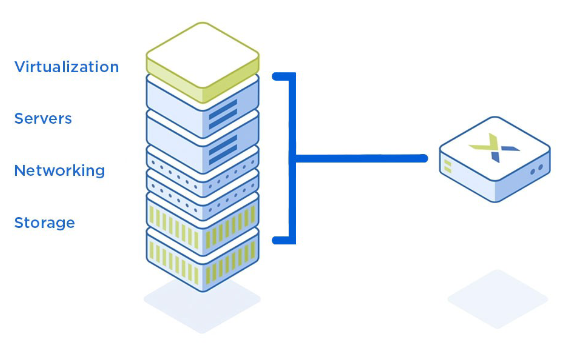
\includegraphics[width=0.5\linewidth]{SAC_B7_hyperconvergence}
			\label{fig:sacb7hyperconvergence}
		\end{figure}
		
		È un tentativo di condensare in un livello di intelligenza
		unico tutte le funzioni di gestioni del datacenter.
		L'Iperconvergenza è ampiamente utilizzata in contesti cloud e
		consiste in un sistema hardware verticalizzato con già al suo interno tutti
		gli elementi di computazione, storage e
		networking. Sono a tutti gli effetti dei \textbf{piccoli
		datacenter} già testati in modo da non risultare
		colli di bottiglia. Sistemi di questo tipo si
		auto configurano, comportando una riduzione dei costi
		CAPEX e OPEX e un deployment efficiente.
		
		\paragraph{Riduzione della Topologia di Rete - Fabric Computing}\label{riduzione-della-topologia-di-rete}\mbox{}\\
		Consiste nella virtualizzazione delle risorse di rete in modo
		da avere una visione semplificata. Gli elementi di
		switching multipli vengono condensati su un unico
		elemento di switching. L'idea è quella di avere una rete \textit{mesh}
		che interconnette tra loro dispositivi di rete e
		di storage virtualizzando entrambi. Tipicamente viene realizzato mediante le Software Defined Networks. Riducendo tutto ad una mesh la comunicazione tra macchine è particolarmente veloce in quanto vicine. Inoltre, è possibile scalare la rete e riconfigurarla efficacemente in base alle necessità.

		\paragraph{Topi ed Elefanti}\label{topi-e-elefanti}\mbox{}\\
		Sfrutta le caratteristiche del traffico di rete, che nei data center non è uniforme. 
		La terminologia "topi" (breve) ed "elefanti" (lungo) per la durata del flusso fornisce una metafora per il traffico web. Ci sono relativamente pochi elefanti e un gran numero di topi.
		Può accadere quindi che vi siano link sovraccaricati e altri sottoutilizzati.
		Si utilizzano piccoli set di link veloci riconfigurabili dinamicamente in base alla richiesta. In questo modo flussi più grandi verranno su determinati link mentre flussi più piccoli su altri.
		Tipicamente vengono utilizzati collegamenti ottici con switch ottico-meccanici.
		
		\subsection{Progettazione di un Data Center}\label{progettazione-di-un-data-center}
		\subsubsection{Posizione}\label{posizione}
		
		Il posizionamento di un data center è un fattore importante da
		tenere in considerazione. In generale è bene scegliere
		zone economiche, sicure da disastri
		naturali (in America le zone vicino a Las Vegas sono
		sicure, ma non economiche), lontane da impianti
		chimici o nucleari e che non siano obiettivi militari.
		Quando si sceglie dove costruire un data center è inoltre
		importante guardare i costi delle risorse come
		l'energia, le tasse e il
		costo delle risorse umane. Anche questo mercato
		viene mosso dalle tendenze che fanno
		lievitare i prezzi. Anche fattori come il
		clima e la logistica (autostrade,
		trasporto) sono da considerare. Anche la vicinanza
		all'utente è un aspetto da tenere in conto, in quando contribuisce a un
		miglioramento del tempo di risposta dei servizi.
		
		\subsubsection{Sicurezza dei Data Center}\label{sicurezza-dei-data-center}
		Questi sistemi senza un personale adeguato valgono zero. Il
		fattore umano è la maggiore causa di incidenti. Occorre
		fare un analisi del comportamento dei dipendenti,
		prima dell'assunzione e durante il periodo lavorativo.
		Inoltre il personale richiede una certa formazione, ed è
		necessaria una separazione in ruoli. L'accesso
		fisico alle strutture deve essere vietato: i data
		center richiedono entrate controllate con
		sistemi di videosorveglianza e guardie di
		sicurezza. Qualora dovesse essere concesso
		l'accesso questo deve avvenire mediante dei badge
		o dei sistemi di autenticazione con dati biometrici.
		Ciascun dipendente deve disporre dei privilegi di accesso
		minimi per poter svolgere il proprio lavoro.
		
		\subsubsection{Raffreddamento}\label{raffreddamento}
		\begin{figure}[ht]
			\centering
			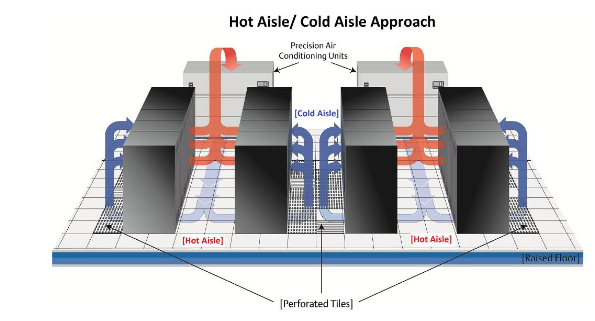
\includegraphics[width=0.5\linewidth]{SAC_B7_cooling}
			\label{fig:sacb7cooling}
		\end{figure}
		
		Il raffreddamento rappresenta il costo maggiore
		per la manutenibilità di un data center. La tecnologia più utilizzata
		per quest'aspetto consiste nell'utilizzo delle \textbf{Computer
		Room Air Conditioner} (CRAC), ovvero di stanze con
		condizionatori enormi. Questi includono un sistema di
		raffreddamento e di filtraggio della polvere (che
		rende meno efficiente la dissipazione del calore). Il
		flusso dell'aria viene gestito in modo da avere
		dell'aria fredda che gira sotto al pavimento e che esce
		attraverso delle piastrelle perforate. I server vengono
		messi tutti rivolti nella stessa direzione e si cerca di creare un
		sistema di corridoi alternati di aria fredda e di aria
		calda. Per evitare la dissipazione del calore dai corridoi caldi
		possono anche essere utilizzati un tettuccio o delle
		tende sopra ai racks. Il riscaldamento è
		un aspetto molto importante perché ha un \textbf{\emph{impatto
		importante sulla vita dei componenti}}. Data la loro importanza anche i
		sistemi di raffreddamento devono essere ridondanti. Deve
		esserci un protocollo di emergenza nei casi in cui uno o
		più condizionatori si spengono.
		
		\begin{quote}
		Google e Facebook: I due colossi,
		essendo il raffreddamento il costo energetico più grande all'interno di
		un data center, hanno cominciato a costruire data center in
		zone con un clima freddo, in modo da poter
		utilizzare l'aria esterna.
		\end{quote}
		
		\subsubsection{Energia}
		L'enorme richiesta di energia dei data center non è dovuta solo alla potenza computazionale ma anche al raffreddamento e nel mondo rappresenta una parte consistente del consumo globale. Sono necessari generatori di corrente nell'ordine delle decine di MW con gruppi di continuità a gasolio per i cali di corrente, sistemi di raffreddamento ridondanti etc.
		
		\newpage
		\section{Gestione dei Data Center}
		La gestione del data center è un problema complesso per la
		quantità di bisogni in gioco, specie alcuni in conflitto tra loro. In
		generale, si deve cercare di \emph{ridurre i costi massimizzando il
		profitto}, il tutto cercando di garantire le SLA (\emph{Service
		Level Agreement}, requisiti di throughput e tempo di risposta che devono essere rispettati dal
		Service Provider nei confronti dei propri clienti). Il problema
		della gestione può essere visto come un \textbf{problema di
		ottimizzazione}, nel quale bisogna tenere conto di diverse
		metriche di performance:
		
		\begin{itemize}
		\tightlist
		\item
		  Key Performance Indicator (KPI): le metriche
		  di performance del sistema
		\item
		  VINCOLI: solitamente requisiti aggiuntivi del sistema (es.
		  tempi di servizio)
		\end{itemize}
		
		\hypertarget{metriche-di-performance}{%
		\subsection{Metriche di Performance}\label{metriche-di-performance}}
		Per descrivere le performance di un data center è possibile considerare
		diversi aspetti:
		
		\begin{itemize}
		\tightlist
		\item
		  Consumo Energetico
		\item
		  SLA
		\item
		  Failure Rate
		\item
		  Utilizzo delle Risorse
		\item
		  Affidabilità / Disponibilità
		\end{itemize}
		\subsubsection{Consumo Energetico}
		Per considerare il consumo energetico di cui ha bisogno un data center è
		possibile pensare alle singole componenti del consumo:
		computazione, networking, storage, e
		cooling. La nuova frontiera tende verso i green
		data center: siccome i data center sono strutture estremamente affamate
		di risorse, sarebbe ideale limitare il consumo di brown energy
		(non rinnovabile), promuovendo il consumo di \emph{energia
		green}.
		
		\subsubsection{Service Level Agreement (SLA)}\label{service-level-agreement-sla}
		
		Il SLA fa riferimento ai requisiti contrattuali che il sistema deve
		rispettare. I requisiti si esprimono solitamente sotto forma di
		\textbf{tempi di risposta}, \textbf{throughput} e
		\textbf{disponibilità} del sistema. Per rappresentare il
		tempo di risposta del sistema è necessario prendere in
		considerazione un intervallo di tempo sensato: una finestra di
		24h non avrebbe senso se il periodo per gran parte del tempo
		durante la giornata è inattivo, per questo viene solitamente calcolato
		in una finestra di pochi minuti. Il tempo di risposta inoltre non può
		essere preso dai log, che tengono conto anche delle \emph{tempistiche
		lato client}. Trattandosi di una variabile aleatoria,
		rappresentata come valore medio o 90-percentile, è
		necessario utilizzare una funzione cumulativa di probabilità
		(integrale della densità di probabilità): ponendo
		sull'asse delle X i valori (istanti di tempo) e
		sull'asse delle Y la probabilità.\\
		\begin{figure}[ht]
			\centering
			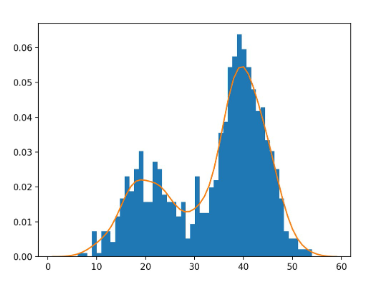
\includegraphics[width=0.7\linewidth]{SAC_B8_sla}
			\label{fig:sacb8sla}
		\end{figure}
		Molto spesso, specialmente per distribuzioni multimodali, si è soliti utilizzare metriche
		come il 90-percentile, che esprimono l’andamento della maggior parte della misura
		per la quale si vuole garantire un determinato SLA.
		Il SLA talvolta può essere garantito all'interno di certe
		soglie di carico. All'aumentare del carico del sistema
		aumenta la probabilità di accodamento delle richieste.
		
		\subsubsection{Utilizzo delle Risorse}\label{utilizzo-delle-risorse}
		Utilizzo della CPU:\\
		La variazione del carico ha un notevole impatto anche sul
		funzionamento della CPU e in particolar modo sulla sua
		temperatura. L'improvvisa accensione e spegnimento di un
		server, può causare uno shock termico, che va a
		accorciare la vita dei componenti.\\
		Il principale parametro per stimare la riduzione di vita dei componenti è il fattore di accelerazione AF:
		\[
		AF = (\frac{f_{STD}}{f_{SM}})^{-m} (\frac{\delta_{STD}}{\delta_{SM}})^{-n}  (e^{\frac{E_a}{K}(1/T^{max}_{STD}-1/T^{max}_{SM})})
		\]
		Dipende dal gradiente di temperatura e dal numero di cicli di potenza.
		L'utilizzo della CPU è un parametro da tenere sotto controllo per le performance del sistema,
		ed è possibile farlo guardando \emph{gli istanti di tempo che questa
		trascorre in stato IDLE}, ma anche considerandone il carico,
		considerando \emph{il numero di processi attivi in coda di esecuzione
		che può scegliere lo schedule}.\\
		La probabilità di un server di essere occupato si esprime come
		\(\rho = \frac{\lambda}{\mu}\). Dove \(\lambda\) è \emph{frequenza di
		arrivo delle richieste} (tasso di arrivo), mentre \(\mu\) è il
		frequenza con cui le richieste vengono soddisfatte (\emph{tasso
		di servizio}).\\
		
		\subsubsection{Utilizzo della Rete}
		Un'altra risorsa del sistema. È possibile studiarne l'utilizzo in
		maniera analoga a quanto visto con la CPU, guardandone
		l'utilizzo dei canali di rete, facendo però attenzione
		al fatto che la banda teorica dei dispositivi non può essere
		raggiunta. Tipicamente, infatti, oltre ad un certo tasso di utilizzazione aumentare il throughput provoca solamente più collisioni, con esiti deleteri per il throughput. Le due metriche per misurare l'utilizzazione sono il throughput (dati trasmessi nel periodo di tempo) e la bandwidth (massimo dei dati che è possibile trasmettere).
		
		\subsection{Modelli di Performance}\label{modelli-di-performance}
		\subsubsection{Modello Energetico}\label{modello-energetico}
		
		Con un modello energetico è possibile misurare il \emph{consumo
		energetico} in un sistema. Nel caso più semplice si considera una
		\textbf{dipendenza lineare} tra l'utilizzazione della CPU e la dissipazione di calore.
		
		Concentrandosi sul consumo energetico della CPU si può adottare il modello \textbf{\emph{Dynamic Voltage
		/ Frequency Scaling}} (DVFS), dove l'energia spesa varia con un
		fattore cubico rispetto alla frequenza del processore. Ulteriori modelli
		di questo tipo possono basarsi sull'utilizzo del disco o sul
		trasferimento dei dati (utilizzo della rete).
		Se gli apparati di rete dedicati hanno costi fissi in termini di consumo energetico non si può dire lo stesso per le reti software defined, dove il traffico incide profondamente sul consumo energetico.
		
		
		
		\subsubsection{Modelli Basati sull'Affidabilità o Disponibilità}\label{modelli-basati-sullaffidabilituxe0-o-disponibilituxe0}
		
		L'affidabilità e la disponibilità del sistema sono
		solitamente usati come vincoli di un modello. Bisogna
		tenere conto di come sono collegati i sistemi: se in
		serie o in parallelo, del loro comportamento in caso di
		failure e del loro livello di replicazione. Inoltre, è
		necessario distinguere se si utilizza un singolo data
		center o molteplici data center, scelta che comporta
		problemi differenti.
		
		Il problema di gestione di più datacenter si articola su due layer:
		\begin{itemize}
			\item come si distribuisce il carico sulla serie di datacenter
			\item come il singolo datacenter reagisce al carico
		\end{itemize}
		Nel caso di più datacenter bisogna capire come \textbf{distribuire il carico} efficacemente su tutti i DC, definire dei \textbf{predittori} del workload futuro, far fronte alla \textbf{località delle richieste} e gestire i molteplici costi delle VM nei DC.
		Nel secondo caso invece l'attenzione è sul singolo DC e su come \textbf{scalarlo}, reagire agli \textbf{errori di predizione} e ai \textbf{burst di traffico}, \textbf{allocare} le VM necessarie e infine gestire la \textbf{sincronizzazione} tra i vari DC.
		
		\subsubsection{Modelli Economici}\label{modelli-economici}
		Se un Provider deve pensare a \textbf{massimizzare} il ricavo, un cliente
		dal canto suo deve \textbf{minimizzare} la spesa. Un Provider tipicamente deve chiedersi come agire nel caso di alto traffico (se prendere in prestito macchine da altri provider, se rivedere il tipo di VM che usa), nel caso di sotto utilizzo dei server (se vendere potenza computazionale con macchine Spot e quanto sia conveniente rispetto al solo tenerle spente). Il problema principale è, però, quello di definire i \textbf{modelli di prezzo} delle varie VM per massimizzarne il ritorno.
		Queste macchine sono:
		
		\begin{itemize}
		\tightlist
		\item
		  Istanze di VM Dedicate: macchine economiche, il cui utilizzo
		  si paga anticipo per essere utilizzate mesi o anni, sempre disponibili
		\item
		  Istanze di VM On Demand: costi alti (\emph{3 x quelle
		  dedicate}), il cui utilizzo si paga per un breve periodo (ore), sempre
		  disponibili
		\item
		  Spot VM: macchine generalmente vendute all'asta con l'intento
		  di fare un profitto (anche se minimo), anche queste pagate per un
		  breve termine, possono essere indisponibili. Se si paga un'ora
		  e la macchina risulta indisponibile per un po' di tempo, quel tempo
		  viene rimborsato.
		\end{itemize}
		
		
		\subsection{Variabili Decisionali}\label{variabili-decisionali}
		\subsubsection{Posizionamento delle VM}\label{posizionamento-delle-vm}
		Il Problema del Posizionamento delle VM può essere visto come un
		\textit{bin packing problem} mono, considerando solo l'utilizzazione CPU, o multidimensionale, considerando anche l'utilizzazione delle altre risorse (RAM, CPU, ecc\ldots). Inoltre, è necessario fare analisi su più istanti temporali in base all'utilizzazione delle risorse che vengono assegnate alle VM. Poiché il problema del bin packing esplode all'aumentare del numero di VM, è possibile semplificare non guardando in termini di numero di
		VM ma di classi di servizio. Categorizzando le macchine in base a determinate alle \textbf{classi} di risorse maggiormente utilizzate si possono ridurre drasticamente le dimensioni del problema a scapito della precisione. Il trade-off è necessario per datacenter che vogliano eseguire predizioni sul traffico in tempi computazionali accettabili.
		
		\begin{quote}
		Si vuole diminuire il Numero di server accesi, dove la formula: \[
		\min{\sum_{s\in S}} O_s
		\] rappresenta il vettore booleano che indica se il server è
		acceso o spento, mentre: \[
		\sum_{s \in S}I_{m,s} = 1
		\] rappresenta un vettore booleano che ha valore \(1\) se
		e solo la macchina \(m\) è allocata sul server \(s\). Una
		macchina può trovarsi su un solo server, quindi deve per forza essere
		\(1\). Si ha che le risorse utilizzate dal server devono essere minori
		delle risorse disponibili sul server (\(V_{r,s}\)) quando questo è
		acceso (\(O_s\)): \[
		\forall s, \forall r, \forall t \quad \sum R_i \cdot r(t) \cdot I_{m,s} < V_{r,s} \cdot O_s
		\]
		\end{quote}

		\subsubsection{Migrazione delle VM}\label{migrazione-delle-vm}
		
		La migrazione consiste nello spostamento di una
		VM da un server a un altro, e si verifica solitamente quando i server
		vengono sotto-utilizzati ($<=20\%$): questi vengono spenti e le macchine spostate
		su altri server più attivi, in modo da poter spegnere i primi
		risparmiando risorse ed energia (\textbf{server consolidation}). Queste variabile vengono identificate
		con i termini \(g_{m,s}^{-}\) quando una \emph{macchina esce da un
		server}, \(g_{m,s}^{+}\) quando entra.
		
		\subsubsection{Ottimizzazione della Rete}\label{ottimizzazione-della-rete}
		
		È necessario mappare il modo in cui le macchine comunicano tra loro in
		maniera ottimale all'interno della rete. Identificando le macchine \textbf{affini} sulla base dello \textbf{scambio di dati} che avviene fra di loro è possibile definire quali devono stare vicine le une alle altre (stesso rack o cluster). Gli altri vincoli, sempre presenti, riguardano le risorse sul server per evitare il sovraccarico e la garanzia di disponibilità.\\
		E' possibile concentrarsi anche sul consumo di energia, l'utilizzo della banda evitando colli di bottiglia e minimizzare il numero di hops in modo da rendere la rete quanto più compatta possibile.
		
		\subsubsection{Orchestrazione}\label{orchestrazione}
		
		Dal punto di vista dell'utilizzatore Cloud, il Deployment del sistema deve considerare i vari
		microservizi, il carico atteso su ciascuno di essi, i requisiti SLA e da decidere quale provider è in grado di far fronte a questi requisiti, sempre con l'obiettivo di \textbf{minimizzare} i costi. Il deployment ottimale viene stabilito in base a  il numero e il tipo di	VM per ciascun servizio, tenendo conto dell'evoluzione del
		suo carico in base alle richieste e ai vincoli SLA.
		
		\subsection{Soluzioni in Ambito Industriale e di Ricerca}\label{soluzioni-in-ambito-industriale-e-di-ricerca}
		\subsubsection{Soluzione Basata sull'Utilizzo}\label{soluzione-basata-sullutilizzo}
		
		Si tratta della ``regola del pollice'' in ambito cloud: viene utilizzata
		per la server consolidation, in modo da evitare
		server sovraccarichi e server sottoutilizzati, viene
		anche utilizzata per le decisioni di scaling e può
		essere affiancata da algoritmi di predizione del carico.
		Si utilizzano due soglie, indicando con \(U\) l'utilizzo
		del server:
		
		\begin{itemize}
		\tightlist
		\item
		  \(U > 80\%\) : parte del carico viene spostato su un nuovo server
		  (bilanciamento del carico).
		\item
		  \(U < 20\%\) : il carico viene distribuito su altri server (\emph{non
		  sovraccarichi}) e il server viene spento (migrazione).
		\end{itemize}
		Per modellare l'andamento dell'utilizzazione in ottica di predizioni, sono spesso utilizzate tecniche di predizioni tramite la \textbf{regressione}.
		I predittori di carico non sono, però, molto utilizzati in ambito industriale,
		perché non sempre il carico e predicibile e talvolta è
		meglio reagire in ritardo piuttosto che reagire male. 
		
		\paragraph{EcoCloud}
		\begin{quote}
		REF Paper. ``Ecocloud''
		
		La migrazione può essere visto come un processo stocastico \textbf{locale} per stabilire se un server deve scaricarsi o se deve accettare nuove macchine. Ad
		ogni VM è associata una probabilità di essere
		oggetto o destinazione di una
		migrazione.
		
		\begin{figure}[ht]
			\centering
			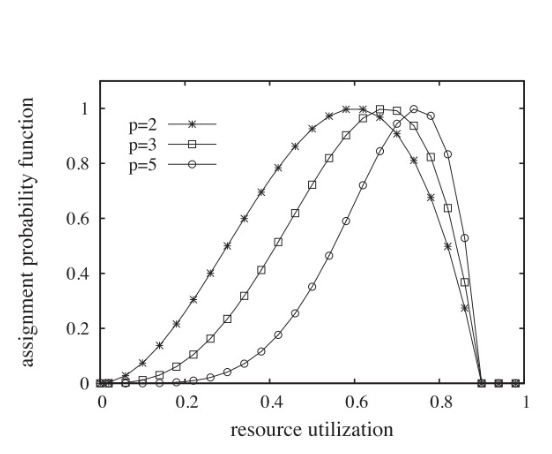
\includegraphics[width=0.7\linewidth]{SAC_B8_ecocloud}
			\label{fig:sacb8ecocloud}
		\end{figure}
		
		Nodi con un'utilizzazione compresa tra il 40\% e il 70\% saranno destinazione di una migrazione per poter consolidare i server. Quando invece la curva di utilizzo raggiunge il 90\% difficilmente tale nodo potrà accoglierne altri senza evitare l'overload e probabilmente subirà una migrazione per poterlo scaricare. Invece quando un nodo ha una bassa utilizzazione è probabile che sarà oggetto di migrazione così da poterlo spegnere. Questo permette la convergenza
		del sistema ad una condizione ideale dove i
		nodi hanno un'utilizzazione medio-alta.
		
		Questa visione è stata confrontata con altre \emph{alternative
		euristiche} come Best Fit Decreasing, che tiene conto di
		molti parametri e una visione completa del data center,
		riuscendo comunque a ottenere buoni risultati.
		\end{quote}
		
		\paragraph{MBFD}
		\begin{quote}
		REF Paper. ``Energy Aware Resource Allocation -
		Modified Best Fit Decresing'' (MBFD)
		
		QUesto algoritmo considera, a differenza del classico best-fit decreasing, macchine virtuali \textbf{eterogenee}.
		Il posizionamento delle VM guarda al \textbf{minimizzare} il
		\textbf{consumo energetico}. La selezione delle macchine da migrare nei server
		in sovraccarico avviene cercando di minimizzare il numero
		di \textbf{migrazioni} e minimizzando il numero di \textbf{accensioni} e
		\textbf{spegnimenti}. Su questa base, vengono scelte per la migrazione le
		macchine più vicine alla soglia, oppure in
		maniera casuale.
		\end{quote}
		
		\paragraph{Hierarchical}
		\begin{quote}
		REF. Paper ``Hierarchical''
		
		Si considerano due tipi di problemi: quelli a lungo termine e quelli a
		breve termine. Quelli a lungo termine consistono nel
		distribuire il carico su più data center cloud, quello a
		breve termine riguarda l'allocazione delle VM. 
		
		In questo genere di rappresentazione, il tempo di risposta viene modellato tramite \textbf{reti di
		code}.
		L’algoritmo \textbf{long term} ragiona con una finestra temporale di un’ora, il tempo di
		riferimento per la frequenza di pagamento delle macchine virtuali (0.056€/hr, ad
		esempio), utilizzando un predittore del traffico in arrivo.
		
		L'algoritmo di soluzione a \textbf{breve termine} segue il principio del \textbf{receding horizon}, in cui la soluzione ottimale si ottiene considerando l'intera finestra temporale, ma l'algoritmo applica solo le decisioni calcolate per il passo temporale più vicino. Il processo di ottimizzazione viene quindi ripetuto considerando il secondo intervallo di tempo come nuovo punto di partenza.
		\end{quote}
		
		\paragraph{VMPlanner}
		\begin{quote}
		REF. Paper ``Optimizing Network Utilization -
		VMPlanner''
		
		Si cerca di posizionare correttamente le VM in modo da
		ridurre i sovraccarichi della rete, in particolare
		alleggerendo la parte core della rete. Essendo un \emph{problema
		NP Hard}, questo viene diviso in sottoproblemi, ciascuno \emph{NP
		completo}:
		
		\begin{enumerate}
		\def\labelenumi{\arabic{enumi}.}
		\tightlist
		\item
		  \textit{Balanced Minimum K-cut problems}: Le macchine virtuali vengono raggruppate in base a diverse classi di traffico
		\item
		  \textit{Quadratic assignement Problem}: I gruppi di traffico vengono mappati sui vari rack all’interno del datacenter
		\item
		  \textit{Multi-commodity flow Problem}: Una volta trovato il posizionamento, viene deciso come viene mappato il flusso di
		  traffico sulla geografia ottenuta
		\end{enumerate}
		
		La soluzione ideale consiste nell'implementazione di
		un'infrastruttura di rete adattiva, in grado di gestire
		i flussi di traffico indipendentemente dalla loro dimensione. I nodi
		all'interno della rete riconoscono il tipo di flusso e
		ricostruiscono le loro matrici per la comunicazione.
		\end{quote}
		
		\paragraph{JCDME}
		\begin{quote}
		REF. Paper ``Joint Minimization of the Energy Cost -
		JCDME''
		
		Approccio che cerca una funzione per minimizzare il \textbf{costo
		energetico} tenendo conto di tanti parametri, a
		ciascuno dei quali viene associato un peso. La
		migrazione è un'operazione costosa in termini
		di consumo energetico, pertanto affinché la decisione
		abbia senso questo costo deve essere spalmato su più unità
		di tempo. Se si ricorre alla migrazione bisogna essere sicuri che in
		seguito il sistema \emph{continuerà a consumare e a richiedere un
		livello più basso di energia per una quantità di tempo che giustifichi
		la scelta}.
		\end{quote}
		\begin{comment}
		    
		
		\section{GCIntro}
		% Work in progress
		\section{WebApp}
		Applicazione creata con Python e Flask.
		Il valore aggiunto dell'approccio con Google Cloud è che non dobbiamo preoccuparci di configurare la rete o l'architettura hardware, macchine virtuali ecc. Le API sono orientate allo sviluppo e possono includere varie funzionalità, anche inerenti al machine learning o map reduce. 
		Da un punto di vista dello sviluppatore è importante concentrarsi sulla gestione delle risorse e sulle performance. E' importante anche configurare bene i parametri di servizio come la gestione delle latenze o minimizzare i costi.
		\subsection{Struttura di un'applicazione}
		\begin{figure}[ht]
		    \centering
		    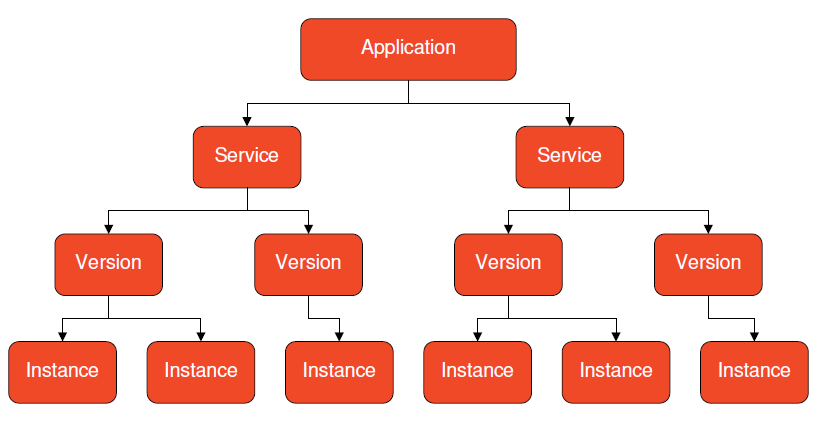
\includegraphics[width=0.8\textwidth]{SAC_C2_01.png}
		\end{figure}
		L'applicazione viene divisa in componenti logici (microservizi), che comunicano tra loro, i componenti condividono le features del motore dell'App. Un servizio consiste in un codice sorgente e un file di configurazione (Es: YAML).
		Ogni servizio può avere pià versioni che possono essere seguite su varie istanze a seconda delle esigenze dello sviluppatore o dell'applicazione.
		Ambiente Virtuale
		Separare le dipendenze del progetto dal cuore delle librerie:
		\begin{itemize}
		    \item Progetti auto contenuti
		    \item Deployment semplificato e riproducibile 
		    \item Utile per il testing
		\end{itemize}
		\section{Storage in Cloud Applications}
		\subsection{Panoramica della memoria}
		Abbiamo diverse opzioni di archiviazione, Google Cloud Platform ha diversi opzioni di database in base al tipo (Relazione o Non relazionale):
		\begin{itemize}
		    \item Cloud SQL: Un'immagine managed, una macchina virtuale con i software già installati per gestire il db
		    \item Cloud Spanner; Utilizzato per gaming, vendite e registro finanziario globale. Possidede uno scaling illimitato con una consistency globale fino al 99,99 \% di availabilty
		    \item AlloyDb for PostgreSQL: Pienamento gestibile, compatibile con PostegreSQL per performances superiori. Utilizzato per grosse migrazioni e applicazioni legacy.
		    \item Bare Meta Solution for Oracle
		    \item BigQuery: Senza un vero server, è altamente scalabile. Processing in real-time e analytics da multicloud.
		    \item Cloud BigTable: Molto performante, pienamente gestito secondo una struttura dati chiave-valore, per operazioni su vasta scala e un ampio carico di lavoro. Personalizzabile, riesce a performare 5 miliardi di richiesta al secondo al suo picco. 
		    \item Firestore
		    \item Firebase Realtime database: Immagazzina e sincronizza i dati in real time. Chat e app per dispositivi mobile.
		    \item MemoryStore
		    \item MongoDB Atlas
		    \item Google Cloud Partner Service: Gestione offerta da open source network, partner di google. 
		\end{itemize}
		\subsection{Google Fire Store}
		
		
		\section{Publisher / Subscriber Systems}
		\subsection{Cloud Pub/Sub}
		Concetti di base: Un topic è quell'elemento di coda che ospita i messaggi, attraverso una Subscription è possibile accedere ai messaggi e ai dati che essi contengono. Ogni messaggio può avere degli attributi in formato chiave valore.
		
		Un publisher crea dei messaggi e li emette verso un topic, un subscriber crea una subscription per la coda e riceve i messaggi. I pattern di comunicazione possono essere di ogni tipo: uno a molti, molti a uno e molti a molti. 
		I messaggi sono immagazzinati in code, possono ricevere degli Acknowledgement che sono sostanzialmente una forma di conferma di lettura, l'Acknowledgement comunica che il messaggio è stato letto e quindi il messaggio viene rimosso dalla coda. 
		
		Ogni applicazione ha degli endpoints ed effettua delle richieste HTTPS.
		Dal punto di vista della subscription abbiamo due modalità:
		\begin{itemize}
		    \item pull: read bloccante, il subscriber attende che vi sia una risposta per la pubblicazione di nuovi messaggi.
		    \item Push: In questo caso viene esposto un url, che sarà invocato quando ci sono nuovi messaggi.
		\end{itemize}
		Casi d'uso:
		\begin{itemize}
		    \item Bilancio del carico in una rete di cluster
		    \item Implementazione di workflow asincroni
		    \item Distribuire eventi di notifica
		    \item
		\end{itemize}
		Prezzi del modello:
		I primi 10 giga sono gratuiti, successivamente vi è un costo di 40\& al Terabyte.
		\end{comment}
		
		\newpage	
		\section{Modelli di decisione}
		\subsection{CBA: Analisi costi e benefici}
		Considerare se un progetto è remunerativo. Si va a calcolare in quanto tempo il mio progetto mi ripaga delle spese iniziali. Quando analizziamo i benefici consideriamo due approcci:
		\begin{itemize}
		    \item Assegnare valori economici a benefici tangibili e intangibili
		    \item Tenere separati i valori finanziari e benefici intangibili
		\end{itemize}
		Metriche di decisione:
		\begin{itemize}
		    \item TCO: Misura dei costi, nessun supporto per analisi complesse.
		    \item CBA: Compara costi e benefici.
		    \item ROI: Quantifica i benefici.
		\end{itemize}
		\subsection{Processo di selezione}
		\begin{itemize}
		    \item 1: Formare un team, progetto e fare un'analisi di ciò che occorre.
		    \item 2: Preparare una definizione dei requisiti.
		    \item 3: Attraverso un processo di selezione intelligente valutare le proposte.
		    \item 4: Valutare una breve lista di fornitori.
		    \item 5: Applicare gli strumenti finanziari per costruire un modello di business per la migliore decisione presa.
		    \item 6: Costruire il documento e negoziare.
		    \item 7: Implementare e tracciare i risultati.
		\end{itemize}
		\subsubsection{Team}
		E' importante che il team sia cross-funzionale e permetta di coprire vari rami di interesse. Alla base di tutto ci deve essere un project manager (lead) che sviluppo un piano di lavoro con definizione delle risorse e delle tempistiche di lavoro. \\
		All'interno dello sviluppo non devono mancare meetings e comunicazione per facilitare la soddisfazioe dei requisiti.
		\subsection{Definizione dei requisiti}
		Documentare tutti i requisiti per il sistema o strumento proposto, dando priorità ai must have e a seguire i nice have e requisti opzionali. 
		E' opportuno poter dare un peso numerico a tutti i requisiti.
		\subsubsection{Processo di selezione}
		Mandare una RFP(Requeste For Proposal) ai venditori target, che più soddisfano le nostre esigenze. Da considerare durante il processo:
		\begin{itemize}
		    \item Qualità del supporto tecnico.
		    \item Rivedere dimostrazioni dai venditori selezionati.
		\end{itemize}
		\subsubsection{Breve lista di fornitori}
		Una volta selezionati i venditori, fissare dei colloqui includendo il team nelle dimostrazioni e determinare se possiamo usare la versione trial del servizio o meno.
		Può essere utile valutare la qualità del servizio, indagando su quella che è la reputazione dell'azienda. 
		\subsubsection{Analisi finanziare}
		Utilizzare le metriche viste prima per trovare la soluzione migliore alle nostre esigenze. Tenere in considerazione:
		\begin{itemize}
		    \item Rapporto costo benefici.
		    \item Ritorno in denaro.
		    \item Costo totale più basso in relazione alla vita dell'investimento.
		\end{itemize}
		\subsubsection{Documento di business}
		Il risultato della metriche utilizzate deve essere sintetizzato in un documento che riporta il sommario di esecuzione, obiettivi e varie raccomandazioni.
		\subsubsection{Implementazione}
		La chiave per il successo in questo caso è scegliere la miglior pratica di project management, definendo un capo, un team multifunzionale e delle priorità.
		\subsection{Focus sul Cloud}
		Il cloud introduce dei cambiamenti al tipico scenario, in quanto i costi di riduzione o di adozione di una tecnologia sono minori grazie al cloud computing.
		Gli utenti possono configurare il loro sistema in base alle loro esigenze e la scalabilità avviene nel giro di minuti anzichè in giorni.
			\end{document}